% LaTeX source for textbook ``Physical Modeling in MATLAB''
% Copyright 2018 Allen B. Downey and W. Craig Scratchley
%
% License: Creative Commons Attribution-NonCommercial 
% 4.0 Unported License.
% http://creativecommons.org/licenses/by-nc/4.0/
%
% Labels within this document are prefixed with
% "ex:", "eqn:", "chpt:", "sect:"
% to indicate an example, equation, chapter, or section, respectively.

\documentclass[
    %oneside,   % uncomment this for static margins (as well as below)
]{book}

\usepackage[
    % Set margins here
    letterpaper,
    %left=1.5in, % uncomment these two, and comment out next two for static margins
    %right=1.5in,
    inner=1.6in,
    outer=1.00in,
    top=1.25in,
    bottom=1.25in,]{geometry}
\usepackage[symbol*]{footmisc}
\usepackage[toc,page]{appendix}
\usepackage{amsmath, amsthm, amssymb}
\usepackage{bm}
\usepackage{bookmark}
\usepackage{exercise}
\usepackage{fancyhdr}
\usepackage{graphicx}
%\usepackage{hevea}
\usepackage{hyperref}
\usepackage{ifthen}
\usepackage{upquote}
\usepackage{url}

% Tell compiler to make the index
\usepackage{imakeidx}
\makeindex

% Include index in ToC
\usepackage[totoc]{idxlayout}

% Configure exercise environment
\numberwithin{Answer}{chapter}
\numberwithin{Exercise}{chapter}
\renewcommand{\ExerciseHeader}{%
  \par\noindent
  \textbf{\ExerciseName~\ExerciseHeaderNB\ExerciseHeaderTitle\ExerciseHeaderOrigin}%
  \par\nopagebreak
}

% colors for code listings and output
\usepackage{xcolor}
\definecolor{bgcolor}{HTML}{FAFAFA}
\definecolor{comment}{HTML}{007C00}
\definecolor{keyword}{HTML}{0000FF}
\definecolor{strings}{HTML}{B20000}

% syntax highlighting in code listings
\usepackage{textcomp}
\usepackage{listings}
\lstset{
    language=matlab,
    basicstyle=\ttfamily,
    backgroundcolor=\color{bgcolor},
    commentstyle=\color{comment},
    keywordstyle=\color{keyword},
    stringstyle=\color{strings},
    columns=fullflexible,
    emph={label},  % keyword?
    keepspaces=true,
    showstringspaces=false,
    upquote=true,
    xleftmargin=15pt,  % \parindent
    framexleftmargin=3pt,
    aboveskip=\parskip,
    belowskip=\parskip
}

% code listing environments
\lstnewenvironment{code}
{\minipage{\linewidth}}
{\endminipage}

\lstnewenvironment{stdout}
{\lstset{commentstyle=,keywordstyle=,stringstyle=}\minipage{\linewidth}}
{\endminipage}

% inline syntax formatting
\newcommand{\mcode}[1]{\lstinline{#1}}%{

% to get siunitx
% sudo apt-get install texlive-science
\usepackage{siunitx}
\sisetup{per-mode=symbol}

%% Add pdf metadata here
\hypersetup{
    pdftitle={Physical Modeling in MATLAB v. 2},
    pdfsubject={MATLAB programming},
    pdfauthor={Allen B. Downey, W. Craig Scratchley},
    pdfcreator={LaTeX},
}

% use mcode as a synonym for verb, for inline MATLAB code
%\newcommand{\mcode{1}}{\mintinline{matlab}{#1}}



%% Macros and redefinitions

% Generate the registered trademark symbol
\newcommand{\myreg}{\textsuperscript{{\tiny \textregistered}}}

% Use bold style for vectors
\renewcommand{\vec}[1]{\bm{\mathbf{#1}}}

% Define style for unit vectors. Complexity needed to display i_hat and
% j_hat correctly
\newcommand{\uveci}{{\bm{\hat{\textnormal{\bfseries\i}}}}}
\newcommand{\uvecj}{{\bm{\hat{\textnormal{\bfseries\j}}}}}
\newcommand{\uvec}[1]{%
    \ifthenelse{\equal{#1}{i}}%
        {\uveci}{%
    \ifthenelse{\equal{#1}{j}}%
        {\uvecj}{%
    {\bm{\hat{\mathbf{#1}}}}% default case
}}}

% Define style for the norm of a vector
\newcommand{\norm}[1]{\lvert #1 \rvert}

% Create an "array" for the 9 theorems of debugging. Depends on ifthen
% package above. (The 'xstring' package does this more elegantly, but
% doesn't work with hevea.) This way we only need to change the theorems
% in one place to change them everywhere.
\newcommand{\displaythrm}[1]{%
    \ifthenelse{\equal{#1}{1}}%
        {Readable code is debuggable code.}{%
    \ifthenelse{\equal{#1}{2}}%
        {The only thing worse than getting an error message is {\em
         not} getting an error message.}{%
    \ifthenelse{\equal{#1}{3}}%
        {Be sure that the code you are running
         is the code you think you are running.}{%
    \ifthenelse{\equal{#1}{4}}%
        {Error messages tell you where the problem was discovered,
         not where it was caused.}{%
    \ifthenelse{\equal{#1}{5}}%
        {The best way to avoid a bug is to make it impossible.}{%
    \ifthenelse{\equal{#1}{6}}%
        {The best kind of debugging is the kind you don't have to do.}{%
    \ifthenelse{\equal{#1}{7}}%
        {The worst bugs aren't in your code; they are in your head.}{%
    \ifthenelse{\equal{#1}{8}}%
        {Finding a hard bug requires reading, running, ruminating,
         and sometimes retreating.  If you get stuck on one of these
         activities, try the others.}{%
    \ifthenelse{\equal{#1}{9}}%
        {Error messages sometimes tell you what's wrong, but they
         seldom tell you what to do (and when they try, they're usually
         wrong).}{%
    {}% default case
}}}}}}}}}}% all the closing braces for displaythrm

% Define the title and version in one place here
\newcommand{\thetitle}{Physical Modeling in MATLAB\myreg}
\newcommand{\theversion}{2.3.0}

% TODO: add documentation here - what does this do?
\renewcommand{\chaptermark}[1]{\markboth{#1}{}}
\renewcommand{\sectionmark}[1]{\markright{\thesection\ #1}{}}

% TODO: add documentation here - what does this do?
\renewcommand\MakeUppercase{}

%% End of macros+redefinitions

% TODO: document the below commands. Not quite sure what they do.

\sloppy

\pagestyle{fancyplain}

\lhead[\fancyplain{}{\bfseries\thepage}]%
      {\fancyplain{}{\bfseries\rightmark}}
\rhead[\fancyplain{}{\bfseries\leftmark}]%
      {\fancyplain{}{\bfseries\thepage}}
\cfoot{}

%\newenvironment{code}{\vspace{0.0\parskip} \begin{lstlisting}}{\end{lstlisting} \vspace{0.0\parskip}}

%\newenvironment{code}{\begin{lstlisting}}{\end{lstlisting}}

% these styles get translated in CSS for the HTML version
% \newstyle{a:link}{color:black;}
%\newstyle{p+p}{margin-top:1em;margin-bottom:1em}
%\newstyle{img}{border:0px}

% change the arrows
%\setlinkstext
%  {\imgsrc[ALT="Previous"]{back.png}}
%  {\imgsrc[ALT="Up"]{up.png}}
%  {\imgsrc[ALT="Next"]{next.png}}

%% End of latex configuration

%% Start of the book
\begin{document}

% No chapter numbering, etc. for the title + preface
\frontmatter

% Define stuff to use for title page here
\title {\thetitle}
\author {Allen B. Downey\\
\\
\\
\\
Version 2 Contributor\\
\\
W. Craig Scratchley\\}
\date {Version \theversion}

\sloppy
%\setlength{\topmargin}{-0.375in}
%\setlength{\oddsidemargin}{0.0in}
%\setlength{\evensidemargin}{0.0in}

% Uncomment these to center on 8.5 x 11
%\setlength{\topmargin}{0.625in}
%\setlength{\oddsidemargin}{0.875in}
%\setlength{\evensidemargin}{0.875in}

%\setlength{\textheight}{7.8in}

\setlength{\headsep}{3ex}
\setlength{\parindent}{0.0in}
\setlength{\parskip}{1.7ex plus 0.5ex minus 0.5ex}
\renewcommand{\baselinestretch}{1.02}

% see LaTeX Companion page 62
\setlength{\topsep}{-0.0\parskip}
\setlength{\partopsep}{-0.5\parskip}
\setlength{\itemindent}{0.0in}
\setlength{\listparindent}{0.0in}

% see LaTeX Companion page 26
% these are copied from /usr/local/teTeX/share/texmf/tex/latex/base/book.cls
% all I changed is afterskip

\makeatletter

\renewcommand{\section}{\@startsection
    {section} {1} {0mm}%
    {-3.5ex \@plus -1ex \@minus -.2ex}%
    {0.7ex \@plus.2ex}%
    {\normalfont\Large\bfseries}}
\renewcommand\subsection{\@startsection {subsection}{2}{0mm}%
    {-3.25ex\@plus -1ex \@minus -.2ex}%
    {0.3ex \@plus .2ex}%
    {\normalfont\large\bfseries}}
\renewcommand\subsubsection{\@startsection {subsubsection}{3}{0mm}%
    {-3.25ex\@plus -1ex \@minus -.2ex}%
    {0.3ex \@plus .2ex}%
    {\normalfont\normalsize\bfseries}}

% The following line adds a little extra space to the column
% in which the Section numbers appear in the table of contents
\renewcommand{\l@section}{\@dottedtocline{1}{1.5em}{3.0em}}
\setcounter{tocdepth}{1}

\makeatother

\newcommand{\beforefig}{\vspace{1.3\parskip}}
\newcommand{\afterfig}{\vspace{-0.2\parskip}}

\newcommand{\beforeverb}{\vspace{0.6\parskip}}
\newcommand{\afterverb}{\vspace{0.6\parskip}}

\newcommand{\adjustpage}[1]{\enlargethispage{#1\baselineskip}}


% Note: the following command seems to cause problems for Acroreader
% on Windows, so for now I am overriding it.
%\newcommand{\clearemptydoublepage}{
%            \newpage{\pagestyle{empty}\cleardoublepage}}
\newcommand{\clearemptydoublepage}{\cleardoublepage}

%\newcommand{\blankpage}{\pagestyle{empty}\vspace*{1in}\newpage}
\newcommand{\blankpage}{\vspace*{1in}\newpage}

% HEADERS

\renewcommand{\chaptermark}[1]{\markboth{#1}{}}
\renewcommand{\sectionmark}[1]{\markright{\thesection\ #1}{}}

\lhead[\fancyplain{}{\bfseries\thepage}]%
      {\fancyplain{}{\bfseries\rightmark}}
\rhead[\fancyplain{}{\bfseries\leftmark}]%
      {\fancyplain{}{\bfseries\thepage}}
\cfoot{}

\pagestyle{fancyplain}


% turn off the rule under the header
%\setlength{\headrulewidth}{0pt}

% the following is a brute-force way to prevent the headers
% from getting transformed into all-caps
\renewcommand\MakeUppercase{}

% Exercise environment
\newtheoremstyle{myex}% name
     {9pt}%      Space above
     {9pt}%      Space below
     {}%         Body font
     {}%         Indent amount (empty = no indent, \parindent = para indent)
     {\bfseries}% Thm head font
     {}%        Punctuation after thm head
     {0.5em}%     Space after thm head: " " = normal interword space;
           %       \newline = linebreak
     {}%         Thm head spec (can be left empty, meaning `normal')

\theoremstyle{myex}

%\begin{latexonly}

%% Title page

\newgeometry{centering}
    \maketitle
\restoregeometry

% License page for latex code

\vspace{2in}

\begin{center}
    {\Large \thetitle}
\end{center}

\vspace{21em}

Copyright \textcopyright \, 2018 Allen Downey

\vspace{0.5em}

\begin{flushleft}
Green Tea Press       \\
9 Washburn Ave \\
Needham MA 02492
\end{flushleft}

\vspace{0.5em}

Copyright \textcopyright \, 2018 W. Craig Scratchley

\vspace{0.5em}

\begin{flushleft}
School of Engineering Science\\
Simon Fraser University\\
8888 University Drive\\
Burnaby, BC V5A 1S6
\end{flushleft}

\vspace{2em}

Permission is granted to copy, distribute, and/or modify this document
under the terms of the Creative Commons Attribution-NonCommercial 4.0 Unported
License, which is available at \url{http://creativecommons.org/licenses/by-nc/4.0/}.

MATLAB\myreg is a registered trademark of The
Mathworks, Inc.  The Mathworks does not warrant the accuracy
of this book.

\vspace{2em}

This book was typeset by the authors using \LaTeX
among other free, open-source software.

Version 2.0.0 of \thetitle was released in 2017. The active Git
    repository for this book is at
    \url{https://github.com/AllenDowney/PhysicalModelingInMATLAB}

% Craig, am I right that we have converged on my repo for all development?

Copying, distributing, and contributing to \thetitle is encouraged.
The above repository is the easiest entry point for this.

\chapter{Preface to Version 2}
% \end{latexonly}

I've used \textit{\thetitle} as the course
textbook for ``Introduction to Engineering Analysis'' at Simon Fraser
University (SFU) for the past two years. This book is ideal for
first-year undergraduate students because of its clear presentation and
delayed introduction to matrices---which is pivotal for students
just beginning linear algebra.  My first time using this book was an
absolute pleasure---Downey has the talent to make ordinarily dry
subjects come to life; however, it became apparent, both from my direct
experience teaching and from the feedback of my students, that
significant revisions were needed to fully realize the effectiveness
of this book.

Hence the creation of Version 2 of this book: the entire text
has been edited for clarity, correctness, and readibility; the
arrangement of chapters and sections has been improved;
and all MATLAB\myreg output has been made consistent
with the 2016 releases. There are many other
changes, too, but there's only so much room here.

Many thanks go to Allen Downey for writing this book and making it open
source; to SFU for funding this revision through the Open Educational
Resources Grant; and to the following students for helping me transform
this book into its current form: Zhen Gang Xiao, Zavier Patrick Aguila,
Michael Cline, and Matt Wiens.

\noindent W. Craig Scratchley
\\
\noindent Vancouver, BC
\\
{\tt craig\_scratchley@alumni.sfu.ca}

\newpage

\chapter{Preface}

% TODO: Let's unify the two prefaces and update with information about
% the revised book, Octave, and instructions for working with the code.

Most books that use MATLAB are aimed at readers who know how
to program.  This book is for people who have never programmed
before.

As a result, the order of presentation is unusual.  The book starts
with scalar values and works up to vectors and matrices very
gradually.  This approach is good for beginning programmers, because
it is hard to understand composite objects until you understand basic
programming semantics.  But there are some challenges:

\begin{itemize}

\item The MATLAB documentation is written in terms of matrices,
and so are the error messages.
To mitigate this problem, the book explains the necessary
vocabulary early and deciphers some of the messages that
beginners find confusing.

\item Many of the examples in the first half of the book are
not idiomatic MATLAB code.  We address this problem in the second
half by translating the examples into a more standard style.

\end{itemize}

The book puts a lot of emphasis on functions, in part because they are
an important mechanism for controlling program complexity, and also
because they are useful for working with MATLAB tools like {\tt fzero}
and {\tt ode45}.

We assume that readers know calculus and physics at the high school level, but not linear algebra.
We present differential equations and use numerical methods to solve them, but we don't assume that readers have seen differential equations before.

There are small exercises within each chapter, and a few larger
exercises at the end of some chapters.

\section*{Working with the code}

Installing MATLAB.

Working with LiveScripts

Installing Octave and JupyterLab

If you are using this book with Octave, we strongly recommend that you install Anaconda, which is a package management system that makes it easy to work with Octave and supporting software.

Anaconda installs everything at the user level, so you can install it without admin or root permissions.  Follow the instructions for your operating system at \url{https://www.anaconda.com/download}.

\begin{code}
conda create --name ModSimMatlab
conda activate ModSimMatlab
conda install -c conda-forge octave octave_kernel
\end{code}

Might have to add this:

\begin{code}
export QT_STYLE_OVERRIDE=gtk2
\end{code}


Working with notebooks.


If you have suggestions and corrections, please send them to
{\tt downey@allendowney.com}.

% TODO: Update this to send comments to Craig?


\newpage

\section*{Contributor's list}

People who have found errors and helped us improve this book include
Michael Lintz, 
Kaelyn Stadtmueller, 
Roydan Ongie, 
Keerthik Omanakuttan, 
ietro Peterlongo, 
Li Tao, 
Steven Zhang, 
Elena Oleynikova, 
Kelsey Breseman, 
Philip Loh, 
Harold Jaffe, 
Vidie Pong, 
Nik Martelaro, 
Arjun Plakkat, 
Zhen Gang Xiao, 
Zavier Patrick Aguila, 
Michael Cline.

Matt Wiens revised several sections of the book.

\newpage

% Table of contents

\pdfbookmark[chapter]{\contentsname}{toc}
\tableofcontents

\mainmatter

\chapter{Modeling}

This book is about modeling and simulation of physical systems.  
The following diagram shows what I mean by ``modeling":

\index{modeling}

\vspace{0.2in}
\centerline{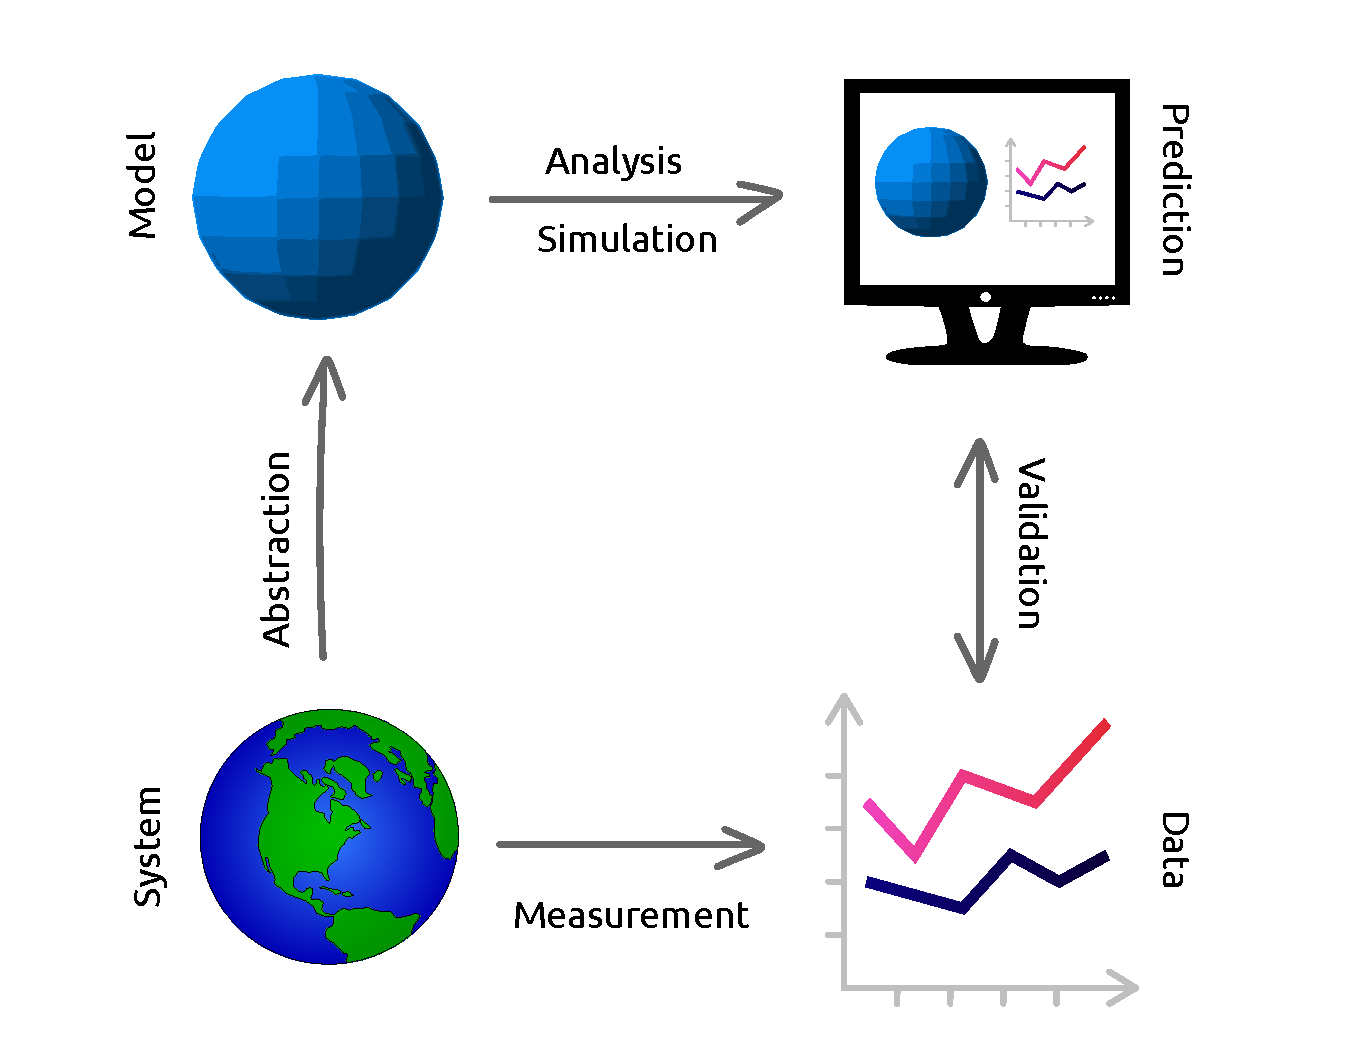
\includegraphics[height=2.8in]{figs/modeling_framework.pdf}}

Starting in the lower left, the {\bf system} is something in the real world we are interested in.  Often, it is something complicated, so we have to decide which details can be left out; removing details is called {\bf abstraction}.

\index{system}

The result of abstraction is a {\bf model}, which is a description of the system that includes only the features we think are essential.  A model can be represented in the form of diagrams and equations, which can be used for mathematical {\bf analysis}.  It can also be implemented in the form of a computer program, which can run {\bf simulations}.

\index{model}
\index{abstraction}
\index{analysis}

The result of analysis and simulation might be a {\bf prediction} about what the system will do, an {\bf explanation} of why it behaves the way it does, or a {\bf design} intended to achieve a purpose.

\index{prediction}
\index{explanation}
\index{design}

We can {\bf validate} predictions and test designs by taking {\bf measurements} from the real world and comparing the {\bf data} we get with the results from analysis and simulation. 

\index{validation}
\index{data}

For any physical system, there are many possible models, each one including and excluding different features, or including different levels of detail.  The goal of the modeling process is to find the model best suited to its purpose (prediction, explanation, or design).

\index{iterative modeling}

Sometimes the best model is the most detailed.  If we include more features, the model is more realistic, and we expect its predictions to be more accurate.

\index{realism}

But often a simpler model is better.  If we include only the essential features and leave out the rest, we get models that are easier to work with, and the explanations they provide can be clearer and more compelling.

\index{simplicity}

As an example, suppose someone asked you why the orbit of the Earth is nearly elliptical.  If you model the Earth and Sun as point masses (ignoring their actual size), compute the gravitational force between them using Newton's law of universal gravitation, and compute the resulting orbit using Newton's laws of motion, you can show that the result is an ellipse.

\index{orbit}
\index{ellipse}

Of course, the actual orbit of Earth is not a perfect ellipse, because of the gravitational forces of the Moon, Jupiter, and other objects in the solar system, and because Newton's laws of motion are only approximately true (they don't take into account relativistic effects).

\index{Newton}
\index{relativity}

But adding these features to the model would not improve the explanation; more detail would only be a distraction from the fundamental cause.  However, if the goal is to predict the position of the Earth with great precision, including more details might be necessary.  

Choosing the best model depends on what the model is for.  It is usually a good idea to start with a simple model, even if it is likely to be too simple, and test whether it is good enough for its purpose.  Then you can add features gradually, starting with the ones you expect to be most essential.  This process is called {\bf iterative modeling}.

Comparing results of successive models provides a form of {\bf internal validation}, so you can catch conceptual, mathematical, and software errors.  And by adding and removing features, you can tell which ones have the biggest effect on the results, and which can be ignored.

\index{internal validation}
\index{validation!internal}
\index{external validation}
\index{validation!external}

Comparing results to data from the real world provides {\bf external validation}, which is generally the strongest test.

The focus of this book is simulation, and the primary tool we will use is MATLAB.

\section{MATLAB}
\label{sect:calc}

At heart, MATLAB is a glorified calculator.  When you start MATLAB
you will see a window
entitled {\sf MATLAB} that contains smaller windows entitled {\sf
Current Folder}, {\sf Command Window}, and {\sf Workspace}.
In Octave, {\sf Current Folder} is called {\sf File Browser}.

The Command Window runs the {\bf interpreter}, which allows you
to type {\bf commands}, then executes them and prints the
result.

Initially, the Command Window contains a welcome message with information
about the version of the software you are running, followed by a {\bf prompt}:

\begin{code}
>>
\end{code}

This symbol prompts you to enter a command.

The simplest kind of command is a mathematical {\bf expression},
like {\tt 2 + 1}).

If you type an expression and then press Enter (or Return), MATLAB
{\bf evaluates} the expression and prints the result.

\begin{code}
>> 2 + 1
ans = 3
\end{code}

Just to be clear: in this example, MATLAB displayed {\tt >>}; I
typed {\tt 2 + 1} and then hit Enter, and MATLAB displayed {\tt ans = 3}.

In this expression, the plus sign is an {\bf operator} and the numbers {\tt 2} and {\tt 1} are {\bf operands}.

An expression can contain any number of operators and operands.  You
don't have to put spaces between them; some people do and some people
don't.

\begin{code}
>> 1+2+3+4+5+6+7+8+9
ans = 45
\end{code}

Speaking of spaces, you might have noticed that MATLAB puts a blank
line between {\tt ans =} and the result.  In many of my examples I will leave
it out to save room.

The other arithmetic operators are pretty much what you would expect.
Subtraction is denoted by a minus sign, {\tt -}; multiplication by
an asterisk, {\tt *}; division by a forward slash, {\tt /}.

\begin{code}
>> 2*3 - 4/5
ans = 5.2000
\end{code}

Another common operator is exponentiation, which uses the \verb+^+
symbol, sometimes pronounced ``carat'' or ``hat''.  So 2 raised to the
16th power is

\begin{code}
>> 2^16
ans = 65536
\end{code}

The order of operations is what you would expect from basic algebra:
exponentiation happens before multiplication and division, and multiplication and division happen before addition and subtraction.
If you want to override the order of operations, you can use parentheses.

\index{operations!order of}


\begin{code}
>> 2 * (3-4) / 5
ans = -0.4000
\end{code}

When I added the parentheses I also changed the spacing to make the
grouping of operands clearer to a human reader.  This is the first
of many style guidelines I will recommend for making your programs
easier to read.  Style doesn't change what the program does; the MATLAB
interpreter doesn't check for style.  But human readers do, and the
most important human who will read your code is you.

And that brings us to the First Theorem of Debugging:

\begin{quote}
\displaythrm{1}
\end{quote}

It is worth spending time to make your code pretty; it will save
you time debugging!


\section{Math functions}

MATLAB knows how to compute pretty much every math function you've
heard of.  It knows all the trigonometric functions; here's how you
use them:

\index{Math functions!trigonometric}

\begin{code}
>> sin(1)
ans = 0.8415
\end{code}

This command is an example of a {\bf function call}.  The name of the
function is {\tt sin}, which is the usual abbreviation for the
trigonometric sine.  The value in parentheses is called the {\bf argument}.

The trig functions {\tt sin}, {\tt cos}, {\tt tan}---among many
others---work in radians.\footnote{MATLAB also provides trig functions
that work in degrees. For example, {\tt sind},{\tt cosd}, and {\tt
tand} compute the sine, cosine, and tangent of an angle given in
degrees.}

Some functions take more than one argument, in which case they are
separated by commas.  For example, {\tt atan2} computes the inverse
tangent, which is the angle in radians between the positive x-axis and
the point with the given $y$ and $x$ coordinates.

\begin{code}
>> atan2(1,1)
ans = 0.7854
\end{code}

If that bit of trigonometry isn't familiar to you, don't worry about
it.  It's just an example of a function with multiple arguments.

MATLAB also provides exponential functions\index{Math functions!exponential}, like {\tt exp}, which computes $e$ raised to the given power.  So {\tt exp(1)} is just $e$.

\begin{code}
>> exp(1)
ans = 2.7183
\end{code}

The inverse of {\tt exp} is {\tt log}\index{Math functions!logarithmic}, which computes the logarithm base $e$:

\begin{code}
>> log(exp(3))
ans = 3
\end{code}

This example also demonstrates that function calls can be {\bf nested};
that is, you can use the result from one function as an argument for
another.

More generally, you can use a function call as an operand in an expression.

\begin{code}
>> sqrt(sin(0.5)^2 + cos(0.5)^2)
ans = 1
\end{code}

As you probably guessed, {\tt sqrt} computes the square root.

There are lots of other math functions, but this is not meant to
be a reference manual.  To learn about other functions, you should
read the documentation.


\section{Documentation}

MATLAB comes with two forms of online documentation, {\tt help}
and {\tt doc}.\index{Documentation!{\tt doc} and {\tt help}}

The help command works completely in the Command Window; just 
type {\tt help} followed by the name of a command.

\begin{code}
>> help sin
 sin    Sine of argument in radians.
    sin(X) is the sine of the elements of X.
 
    See also asin, sind, sinpi.
\end{code}

Some documentation uses vocabulary we haven't covered yet.  
For example, ``the elements of X'' will likely not make sense until
we get to vectors and matrices a few chapters from now.

The {\tt doc} pages are often better for people new to MATLAB.  
If you type {\tt doc sin}, a browser window appears with more detailed information about the function, including examples of how to use it.  The examples often
use vectors and matrices, so they may not make complete sense yet, 
but you can get a preview of what's coming.


\section{Variables}

One of the features that makes MATLAB more powerful than a calculator
is the ability to give a name to a value.  A named value is called
a {\bf variable}.

MATLAB comes with a few predefined variables.\index{Variables!predefined}  For
example, the name {\tt pi} refers to the
mathematical quantity $\pi$, which is approximately

\begin{code}
>> pi
ans = 3.1416
\end{code}

And if you do anything with complex numbers, you might find it
convenient that both {\tt i} and {\tt j} are predefined as the square
root of $-1$\index{Complex numbers!imaginary unit}.

You can use a variable name anywhere you can use a number; for example, as
an operand in an expression:

\begin{code}
>> pi * 3^2
ans = 28.2743
\end{code}

Or as an argument to a function:

\begin{code}
>> sin(pi/2)
ans = 1

>> exp(i * pi)
ans = -1.0000 + 0.0000i
\end{code}

As the second example shows, many MATLAB functions work with
complex numbers.  This example demonstrates Euler's Equality\index{Complex numbers!Euler's Equality}:
$e^{i \pi} = -1$.

Whenever you evaluate an expression, MATLAB assigns the result to
a variable named {\tt ans}.  You can use {\tt ans} in a subsequent
calculation as shorthand for ``the value of the previous expression''.

\begin{code}
>> 3^2 + 4^2
ans = 25

>> sqrt(ans)
ans = 5
\end{code}

But keep in mind that the value of {\tt ans} changes every time
you evaluate an expression.


\section{Assignment statements}

You can create your own variables, and give them values, with
an {\bf assignment statement}.  The assignment operator is the
equals sign, {\tt =}\index{Variables!assignment}.

\begin{code}
>> x = 6 * 7
x = 42
\end{code}

This example creates a new variable named {\tt x} and assigns it the
value of the expression {\tt 6 * 7}.  MATLAB responds with the
variable name and the computed value.

In every assignment statement, the left side has to be a legal variable name.  The right side can be any expression, including function calls.

Almost any sequence of lower and upper case letters is a legal
variable name, as long as the name does not exceed 63 characters.  
Digits are also legal, but not at the beginning of the name.
Some punctuation is also legal, but the underscore,
\verb"_", is the only commonly-used punctuation mark.  
Spaces are not allowed.  Variable names are
``case sensitive'', so {\tt x} and {\tt X} are different variables.

\begin{code}
>> fibonacci0 = 1;

>> LENGTH = 10;

>> first_name = 'bob'
first_name = bob
\end{code}

The first two examples demonstrate the use of the semi-colon\index{Syntax!semi-colon}, which
suppresses the output from a command.  In this case MATLAB creates the
variables and assigns them values, but displays nothing.

The third example demonstrates that not everything
in MATLAB is a number.  A sequence of characters in single quotes is
a {\bf string}.

Although {\tt i}, {\tt j}, and {\tt pi} are predefined, you are free
to reassign them.  It is common to use {\tt i} and {\tt j} for other
purposes, but rare to assign a different value to
{\tt pi}.\index{Complex numbers!imaginary unit}


\section{The workspace}

When you create a new variable, it appears in the {\sf Workspace} window, and it is added to the {\bf workspace}, which is a
set of variables and their values.\index{Variables!workspace}

The {\tt who} command prints the
names of the variables in the workspace.\index{Variables!{\tt who}}

\begin{code}
>> x=5;
>> y=7;
>> z=9;
>> who

Your variables are:

x  y  z
\end{code}

The {\tt clear} command removes specified variables from the workspace

\begin{code}
>> clear x
>> who

Your variables are:

y z
\end{code}

But be careful: if you don't specify any variables, {\tt clear} removes them all.

To display the value of a variable, you can use the {\tt disp} function.

\index{Variables!{\tt disp}}

\begin{code}
>> disp(z)
     9
\end{code}

But it's easier to just type the variable name.

\begin{code}
>> z
z = 9
\end{code}


\section{Why variables?}

Some reasons to use variables are:\index{Variables!reasons for using}

\begin{itemize}

\item To avoid recomputing a value that is used repeatedly.  For
example, if your computation uses $e$ frequently, you might
want to compute it once and save the result\footnote{You don't have to do this in Octave; it is predefined.}.

\begin{code}
>> e = exp(1)
e = 2.7183
\end{code}

\item To make the connection between the code and the underlying
mathematics more apparent.  If you are computing the area of a circle,
you might want to use a variable named {\tt r}:

\begin{code}
>> r = 3
r = 3

>> area = pi * r^2
area = 28.2743
\end{code}

That way your code resembles the familiar formula $a = \pi r^2$.

\item To break a long computation into a sequence of steps.
Suppose you are evaluating a big, hairy expression like this one:
\begin{code}
ans = ((x - 2000000) * sqrt(2 * pi) * 1000000) ^ -1 * ...
exp(-1/2 * (log(x - 2000000) - area)^2 / 1000000^2)
\end{code}

You can use an ellipsis to break the expression into multiple lines.\index{Syntax!ellipses}
Just type {\tt ...} at the end of the first line and continue on the
next.

But often it is better to break the computation into a sequence of
steps and assign intermediate results to variables.

\begin{code}
shiftx = x - 2000000
denom = shiftx * sqrt(2 * pi) * 1000000
temp = (log(shiftx) - area) / 1000000
exponent = -1/2 * temp^2
ans = exp(exponent) / denom
\end{code}

The names of the intermediate variables explain their role in the
computation.  {\tt shiftx} is the value of {\tt x} shifted by 
{\tt 2000000}.  It should be no surprise that {\tt exponent} is the argument of {\tt exp}, and {\tt denom} ends up in the denominator.  Choosing informative names makes the code easier to read and understand, which makes them easier to debug.

\end{itemize}

\section{Errors}

It's early, but now would be a good time to start making errors.
Whenever you learn a new feature, you should try to make as many errors as possible, as soon as possible.

When you make deliberate errors, you see what the error messages are.
Later, when you make accidental errors, you will know what the messages mean.

A common error for beginning programmers is leaving out the {\tt *}
for multiplication.

\begin{code}
>> area = pi r^2
 area = pi r^2
           |
Error: Invalid expression. Check for missing multiplication operator, 
missing or unbalanced delimiters, or other syntax error.
To construct matrices, use brackets instead of parentheses.
\end{code}

The error message indicates that the expression in invalid and suggests several things that might be wrong.  In this case, one of its guesses is right; we are missing a multiplication operator.

Another common error is to leave out the parentheses around the
arguments of a function.  For example, in math notation, it is common
to write something like $\sin \pi$, but not in MATLAB.

\begin{code}
>> sin pi
Undefined function 'sin' for input arguments of type 'char'.
\end{code}

The problem is that when you leave out the parentheses, MATLAB treats
the argument as a string (rather than as an expression).
In this case the error message is helpful, but in other cases the results can be baffling.
For example, if you call {\tt abs}, which computes absolute values, and forget the parentheses, you get a surprising result:

\begin{code}
>> abs pi
ans =  112   105
\end{code}

I won't explain this result; for now, I'll just suggest that you should {\em always} put parentheses around arguments.

This example also demonstrates the Second Theorem of Debugging:

\begin{quote}
\displaythrm{2}
\end{quote}

MATLAB functions are case sensitive, if you type the {\tt sin} function using capital letters in MATLAB, you get an error:

\begin{code}
>> SIN(pi)
Undefined function 'SIN' for input arguments of type 'double'.

Did you mean:
>> sin(pi)
\end{code}

Beginning programmers often hate error messages and do everything they
can to make the messages go away.  Experienced programmers know that error
messages are your friend.  They can be hard to understand, and even
misleading, but it is worth the effort to understand them.

Here's another common error.
If you were translating this mathematical expression into MATLAB:
%
\[ \frac{1}{2 \sqrt \pi} \]
%
You might be tempted to write this:

\begin{code}
1 / 2 * sqrt(pi)
\end{code}

But that would be wrong because of the order of operations.  Division and multiplication are evaluated from left to right, so this expression would multiply {\tt 1/2} by {\tt sqrt(pi)}.

To keep {\tt sqrt(pi)} in the denominator, you could use parentheses:

\begin{code}
1 / (2 * sqrt(pi))
\end{code}

or make the division explicit.

\begin{code}
1 / 2 / sqrt(pi)
\end{code}




\section{Glossary}

\begin{description}

\item[interpreter:] The program that reads and executes MATLAB code.

\item[command:] A line of MATLAB code executed by the interpreter.

\item[prompt:] The symbols the interpreter prints to indicate that it is
waiting for you to type a command.

\item[operator:] One of the symbols, like {\tt *} and {\tt +}, that
represent mathematical operations.

\item[operand:] A number or variable that appears in an expression along
with operators.

\item[expression:] A sequence of operands and operators that specifies
a mathematical computation and yields a value.

\item[value:] The numerical result of a computation.

\item[evaluate:] To compute the value of an expression.

\item[order of operations:] The rules that specify which operations
in an expression are performed first.

\item[function:] A named computation; for example {\tt log10} is the
name of a function that computes logarithms in base 10.

\item[call:] To cause a function to execute and compute a result.

\item[function call:] A kind of command that executes a function.

\item[argument:] An expression that appears in a function call to
specify the value the function operates on.

\item[nested function call:] An expression that uses the result from
one function call as an argument for another.

\item[variable:] A named value.

\item[assignment statement:] A command that creates a new variable
(if necessary) and gives it a value.

\item[string:] A value that consists of a sequence of characters (as
opposed to a number).


\end{description}


\section{Exercises}

\newenvironment{ex}{\begin{Exercise}}{\end{Exercise}}

\begin{ex}
\label{penny}
You might have heard that a penny dropped from the top of the Empire State Building would be going so fast when it hit the pavement that it would be embedded in the concrete; or if it hit a person, it would break their skull.

\index{Empire State Building}
\index{penny}
\index{myth}

We can test this myth by making and analyzing a model.  To get started, we'll assume that the effect of air resistance is small.  This will turn out to be a bad assumption, but bear with me.

If air resistance is negligible, the primary force acting on the penny is gravity, which causes the penny to accelerate downward.
\index{air resistance}

If the initial velocity is 0, the velocity after $t$ seconds is $a t$, and the distance the penny has dropped is
%
\[ h = a t^2 / 2 \]
%
Using algebra, we can solve for $t$:
%
\[ t = \sqrt{ 2 h / a} \]
%
Plugging in the acceleration of gravity, 
$a = \SI{9.8}{\meter\per\second\squared}$, and the height of the Empire State Building, 
$h = \SI{381}{\meter}$, we get 
$t = \SI{8.8}{\second}$.  
Then computing $v = a t$ we get a velocity on impact of $\SI{86}{\meter\per\second}$, which is about 190 miles per hour.  That sounds like it could hurt.

Use MATLAB to perform these computations, and check that you get the same result.
\end{ex}

\begin{ex}
The result in the previous exercise is not accurate it ignores air resistance.  In reality, once the penny gets to about \SI{18}{\meter\per\second}, the upward force of air resistance equals the downward force of gravity, so the penny stops accelerating.  After that, it doesn't matter how far the penny falls; it hits the sidewalk at about \SI{18}{\meter\per\second}, much less than \SI{86}{\meter\per\second}.

As an exercise, compute the time it takes for the penny to reach the sidewalk if we assume that it accelerates with constant acceleration
$a = \SI{9.8}{\meter\per\second\squared}$ until it reaches terminal velocity, then falls with constant velocity until it hits this sidewalk.

The result you get is not exact, but it is a pretty good approximation.

\end{ex}


% chap02
\chapter{Scripts}

\section{M-files}\index{Scripts!M-files}
\label{sect:M-files}

So far we have typed all of our programs ``at the prompt'', which is
fine if you are not writing more than a few lines.  Beyond that,
you will want to store your program in a {\bf script} and then
execute the script.

A script is a file that contains MATLAB code.  These files are
also called ``M-files'' because they use the extension {\tt .m},
which is short for MATLAB.

You can create and edit scripts with any text editor or word processor, but the simplest way is by clicking the {\sf New Script} button in the upper left corner.  A window appears running a text editor specially designed for MATLAB.

Type the following code in the editor:

\begin{code}
x = 5
\end{code}

Then press the {\sf Save} button.  A dialog window should appears where you
can choose the file name and the directory where it should go.  Change
the name to {\tt myscript.m} and save it into any folder you like.

Now press the green {\sf Run} button.  You might get a message that says the script is not found in the current folder.  
If so, click the button that says {\sf Change Folder} and it should run.

You can also run your script from the Command Window: type {\tt myscript} at the prompt and press Enter.  
MATLAB executes your script and displays the result.

\begin{code}
>> myscript
x = 5
\end{code}

When you run a script, MATLAB executes the commands in the M-File, one
after another, exactly as if you had typed them at the prompt.

When you run a script, you should not include the extension {\tt .m}.  If you try, you will get an error message like this:

\begin{code}
>> myscript.m
Undefined variable "myscript" or class "myscript.m".
\end{code}

When you name a new script, try to choose something meaningful and memorable. 

Do not choose a name that is not already in use; if you do, you will replace one of MATLAB's functions with your own (at least temporarily).
You might not notice right away, but you might get some confusing behavior later.

Also, the name of the script cannot contain spaces.  If you create
a file named {\tt my script.m}, MATLAB will complain when you try
to run it:

\begin{code}
>> my script
Undefined function or variable 'my'.
\end{code}

Keeping track of your scripts can be a pain.  To keep things simple,
for now, I suggest putting all of your scripts in one
directory.


\section{Why scripts?}

The most common reasons to use scripts are:

\index{Scripts!reasons for using}

\begin{itemize}

\item When you are writing more than a couple of lines of code, it
might take a few tries to get everything right.  Putting your code
in a script makes it easier to edit than typing it at the prompt.

\item If you choose good names for your scripts, you will be able
to remember which script does what, and you might be able to reuse
a script from one project to the next.

\item If you run a script repeatedly, it is faster to type the
name of the script than to retype the code!

\end{itemize}

But the great power of scripts comes with great responsibility:
you have to make sure that the code you are running is the code you think you are running.

Whenever you start a new script, start with something simple,
like {\tt x=5}, that produces a visible effect.  Then run your script
and confirm that you get what you expect.

When you type the name of a script, MATLAB searches for the script in a {\bf path}, which is a sequence of folders.  If it doesn't find the script in the first folder, it searches the second, and so on.
If you have scripts with the same name in different folders, you could be looking at one version and running another.

If the code you are running is not the code you are looking
at, you will find debugging a frustrating exercise!  And that brings
us to the Third Theorem of Debugging:

\begin{quote}
\displaythrm{3}
\end{quote}


\section{Fibonacci}

The Fibonacci sequence, denoted $F$, is described by the equations
$F_1 = 1$, $F_2 = 1$, and for $i > 2$, $F_{i} = F_{i-1} + F_{i-2}$.
The following expression computes the $n$th Fibonacci number:

\begin{equation}
F_n = \frac{1}{\sqrt{5}}
\left[
\left( \frac{1 + \sqrt{5}}{2} \right)^{n} -
\left( \frac{1 - \sqrt{5}}{2} \right)^{n}
\right]
\end{equation}

We can translate this expression into MATLAB, like this:

\begin{code}
s5 = sqrt(5);
t1 = (1 + s5) / 2;
t2 = (1 - s5) / 2;
diff = t1^n - t2^n;
ans = diff / s5
\end{code}

I use temporary variables like {\tt t1} and {\tt t2} to make the code readable and the order of operations explicit.  The first four lines have a semi-colon at the end, so they don't display anything.  The last line assigns the result to {\tt ans}.

If we save this script in a file named {\tt fibonacci1.m}, we can run it like this:

\begin{code}
>> n = 10
>> fibonacci1
ans = 55.0000
\end{code}

Before calling this script, you have to assign a value to {\tt n}.
If {\tt n} is not defined, you get an error:

\begin{code}
>> clear n
>> fibonacci1
Undefined function or variable 'n'.

Error in fibonacci1 (line 9)
diff = t1^n - t2^n;
\end{code}

This script only works if there is a variable named {\tt n} in the workspace; otherwise, you get an error.

MATLAB tells you what line of the script the error is in, and displays the line.

This information can be helpful, but beware!  MATLAB is telling you
where the error was discovered, not where the error is.  In this
case, the error is not in the script at all, which brings us to the Fourth Theorem of Debugging:

\begin{quote}
\displaythrm{4}
\end{quote}

Often you have to work backwards to find the source of the problem.


\section{Floating-point numbers}

MATLAB uses IEEE double-precision floating-point numbers, which are accurate to about 15 digits of precision.  Most integers can be represented exactly, but most fractions cannot.

For example, if you compute the fraction {\tt 2/3}:

\begin{code}
>> 2/3
ans = 0.6666
\end{code}

The result is only approximate --- the correct answer has an infinite number of 6s. 

It's not as bad as this example makes it seem: MATLAB stores more digits than it shows by default.
You can change the output format to see more digits.

\index{Numbers!{\tt format}}

\begin{code}
>> format long
>> 2/3
ans = 0.666666666666667
\end{code}

In this example, the first 14 digits are correct; the last one has been rounded off.

\index{Numbers!floating point}

Large and small numbers are displayed in scientific notation.  For example, if we use the built in function {\tt factorial} to compute $50!$, we get the following result:

\begin{code}
>> factorial(50)
ans = 3.041409320171338e+64
\end{code}

The {\tt e} in this notation is {\em not} the transcendental number
known as $e$\index{Numbers!$e$}; it is just an abbreviation for ``exponent''.  So
this means that $50!$ is approximately $3.04 \times 10^{64}$.  The
exact solution is a 65-digit integer, but with double-precision floating-point 
we only know the first 16 digits.

If you have the MATLAB Symbolic Math Toolbox installed, you can use a 
different number representation for the calculation and see all the digits of 
the result:

\begin{code}
>> sym(factorial(50))
ans = 30414093201713375576366966406747986832057064836514787179557289984
\end{code}

Compared to the floating-point result, the symbolic result takes substantially more time to compute and space to store in memory.
In this book, we focus on floating-point computation rather than symbolic computation.

You can also enter numbers using scientific notation.

\begin{code}
>> speed_of_light = 3.0e8
speed_of_light = 300000000
\end{code}

Although floating-point can represent very large and small numbers, 
there are limits.  
The predefined variables {\tt realmax} and {\tt realmin}
\index{Numbers!{\tt realmax} and {\tt realmin}} contain the
largest and smallest number magnitudes that MATLAB 
can handle.

\begin{code}
>> realmax
ans = 1.797693134862316e+308

>> realmin
ans = 2.225073858507201e-308
\end{code}

Actually, MATLAB can handle a some numbers with magnitude smaller than 
{\tt realmin}, but with fewer digits of precision.

\begin{code}
>> 1e-323
ans = 9.881312916824931e-324
\end{code}

If a number is too small, MATLAB ``rounds down'' to zero.

\begin{code}
>> 1e-324
ans = 0
\end{code}

If a number -- perhaps the result of a computation -- is too big, 
MATLAB ``rounds up'' to infinity.\index{Numbers!{\tt Inf}}

\begin{code}
>> factorial(170)
ans = 7.257415615307994e+306

>> factorial(171)
ans = Inf
\end{code}

Division by zero also returns {\tt Inf}.

\begin{code}
>> 1/0
ans = Inf
\end{code}

Some older versions of MATLAB give a warning when dividing by zero.
A warning is like an error message without teeth; the computation
is allowed to continue.  Allowing {\tt Inf} to propagate
through a computation doesn't always do what you expect, but if you
are careful with it, {\tt Inf} can be quite useful.

For operations that are truly undefined, MATLAB returns {\tt NaN},
which stands for ``not a number''.\index{Numbers!{\tt NaN}}

\begin{code}
>> 0/0
ans = NaN
\end{code}



\section{Comments}

Along with the commands that make up a program, it is useful to include comments that provide additional information about the
program.  The percent symbol {\tt \%} separates
the comments from the code.\index{Syntax!comments}

\begin{code}
>> speed_of_light = 3.0e8     % meters per second
speed_of_light = 300000000
\end{code}

The comment runs from the percent symbol to the end of the line.
In this case it specifies the units of the value.  In an ideal world,
MATLAB would keep track of units and propagate them through the
computation, but for now that burden falls on the programmer.

Comments have no effect on the execution of the program.  They
are there for human readers.  Good comments make programs more
readable; bad comments are useless or (even worse) misleading.

Avoid comments that are redundant with the code:

\begin{code}
>> x = 5        % assign the value 5 to x
\end{code}

Good comments provide additional information that is not in the
code, like units in the example above, or the meaning of a variable:

\begin{code}
>> p = 0         % position from the origin in meters
>> v = 100       % velocity in meters / second
>> a_g = -9.8    % acceleration due to gravity in meters / second^2
\end{code}

If you use longer variable names, you might not need explanatory
comments, but there is a tradeoff: longer code can become harder
to read.
Also, if you are translating from math
that uses short variable names, it can be useful to make your
program consistent with your math.


\section{Documentation}

Every script should contain a comment that explains
what it does, and what the requirements are for the workspace.  For
example, I might put something like this at the beginning of
{\tt fibonacci1.m}:

\begin{code}
% Computes a numerical approximation of the nth Fibonacci number.  
% Precondition: you must assign a value to n before running this script.
% Postcondition: the result is stored in ans.
\end{code}

A {\bf precondition} is something that must be true when the script
starts in order for it to work correctly.  A {\bf postcondition}
is something that will be true when the script completes.

If there is a comment at the beginning of a script, MATLAB assumes
it is the documentation for the script, so if you type {\tt help
fibonacci1}, you get the contents of the comment (without the percent
signs).

\begin{code}
>> help fibonacci1
  Computes a numerical approximation of the nth Fibonacci number.  
  Precondition: you must assign a value to n before running this script.
  Postcondition: the result is stored in ans.
\end{code}

That way, scripts that you write behave just like predefined scripts.
You can even use the {\tt doc} command to see your comment in the
{\sf Help} window.




\section{Assignment and equality}

\index{Variables!assignment}

In mathematics the equals sign means that the two sides of the
equation have the same value.  In MATLAB an assignment statement
{\em looks} like a mathematical equality, but it's not.

One difference is that the sides of an assignment statement are not
interchangeable.  The right side can be any legal expression, but
the left side has to be a variable, which is called the 
{\bf target} of the assignment.  So this is legal:

\begin{code}
>> y = 1;
>> x = y+1
x = 2
\end{code}

But this is not:

\begin{code}
>> y+1 = x
 y+1 = x
     |
Error: Incorrect use of '=' operator. 
To assign a value to a variable, use '='. 
To compare values for equality, use '=='.
\end{code}

In this case the error message not very helpful.  The problem here is that the expression on the left side is not a valid target for an assignment.

Another difference between assignment and equality is that an assignment statement is only temporary, in the following sense.
When you assign {\tt x = y+1}, you get the
{\em current} value of {\tt y}.  If {\tt y} changes later, {\tt x}
does not get updated.

A third difference is that a mathematical equality is a statement that
may or may not be true.  In mathematics, $y = y+1$ is a statement that
happens to be false for all values of $y$.  
In MATLAB, {\tt y = y+1} is a sensible and useful assignment statement.
It reads the current value of {\tt y}, adds one, and replaces the old value with the new value.

\begin{code}
>> y = 1;
>> y = y+1
y = 2
\end{code}

When you read MATLAB code, you might find it helpful to pronounce
the equals sign ``gets'' rather than ``equals.''  So {\tt x = y+1}
is pronounced ``{\tt x} gets the value of {\tt y} plus one.''


\section{Glossary}

\begin{description}

\item[M-file:] A file that contains a MATLAB program.

\item[script:] An M-file that contains a sequence of MATLAB commands.

\item[search path:] The list of directories where MATLAB looks for
M-files.

\item[workspace:] A set of variables and their values.

\item[precondition:] Something that must be true when the script
starts, in order for it to work correctly.

\item[postcondition:] Something that will be true when the script
completes.

\item[target:] The variable on the left side of an assignment statement.

\item[incremental development:] A way of programming by making a series
of small, testable changes.

\item[scaffolding:] Code you write to help you program or debug, but
which is not part of the finished program.

%\item[unit testing:] A process of testing software by testing each
%component in isolation.

\item[floating-point:] A way to represent numbers in a computer.

\item[scientific notation:] A format for typing and displaying large
and small numbers; e.g. {\tt 3.0e8}, which represents $3.0 \times 10^8$
or 300,000,000.

\item[comment:] Part of a program that provides additional information
about the program, but does not affect its execution.

\end{description}


\section{Exercises}



\begin{ex}
To test your understanding of assignment statements, write a few lines of code that swap the values of {\tt x} and {\tt y}. 
Put your code in a script called {\tt swap} and test it.

If it works correctly, to should be able to run it like this:

\begin{code}
>> x = 1, y = 2
x = 1
y = 2

>> swap

>> x, y
x = 2
y = 1
\end{code}


\end{ex}


\begin{ex}
\label{ex:bikegame}

Imagine that you are the operator of a bike share system with two
locations: Boston and Cambridge.

You observe that every day 5\%
of the bikes in Boston are dropped off in Cambridge, and 3\% of the bikes
in Cambridge get dropped off in Boston.
At the beginning of the month, there are 100 bikes at each location.

Write a script called \verb"bike_update" that updates the number
of bikes in each location from one day to the next.  The precondition
is that the variables {\tt b} and {\tt c} contain the number of bikes
in each location at the beginning of the day.  The postcondition
is that {\tt b} and {\tt c} have been modified to reflect net movement of bikes.

To test your program, initialize {\tt b} and {\tt c} at
the prompt and then execute the script.  The script should display
the updated values of {\tt b} and {\tt c}, but not any intermediate
variables.

Remember that bikes are countable things, so {\tt b} and {\tt c} should always
be integer values.  You might want to use the {\tt round} function
to compute the number of bikes that move each day.

If you execute your script repeatedly, you can simulate the passage
of time from day to day (you can repeat a command by pressing the {\sf Up} arrow and then {\sf Enter}).

What happens to the bikes?  Do they all end up in one place?  Does the system reach an equilibrium, does it oscillate, or does it do something else?

In the next chapter we will see how to execute your script automatically,
and how to plot the values of {\tt a} and {\tt b} over time.
\end{ex}



% chap03
\chapter{Loops}

\section{Updating variables}

In Exercise~\ref{ex:bikegame}, you might have been tempted to write something
like

\begin{code}
b = b - 0.05*b + 0.03*c
c = c + 0.05*b - 0.03*c
\end{code}

But that would be wrong, so very wrong.  Why?  The problem is that
the first line changes the value of {\tt a}, so when the second line
runs, it gets the old value of {\tt b} and the new value of {\tt a}.
As a result, the change in {\tt a} is not always the same as the
change in {\tt b}, which violates the principle of Conversation
of Bikes!

One solution is to use temporary variables {\tt anew} and {\tt bnew}:

\begin{code}
b_new = b - 0.05*b + 0.03*c
c_new = c + 0.05*b - 0.03*c
b = b_new
c = c_new
\end{code}

This has the effect of updating the variables ``simultaneously;'' that
is, it reads both old values before writing either new value.

The following is an alternative solution that
has the added advantage of simplifying the computation:

\begin{code}
b_to_c = 0.05*b - 0.03*c
b = b - b_to_c
c = c + b_to_c
\end{code}

It is easy to look at this code and confirm that it obeys Conversation
of Bikes.  Even if the value of \verb"b_to_c" is wrong, at least the total
number of bikes is right.  And that brings us to the Fifth Theorem of
Debugging:

\begin{quote}
\displaythrm{5}
\end{quote}

In this case, removing redundancy also eliminates the opportunity for
a bug.


\section{Bug taxonomy}

There are four kinds of bugs:

\begin{description}

\item[Syntax error:] You have written a command that cannot
execute because it violates one of the rules of syntax.  For example,
you can't have two operands in a row without an operator, so
\verb+pi r^2+ contains a syntax error.  When the interpreter finds a syntax
error, it prints an error message and stops running your program.\index{Errors!syntax}

\item[Runtime error:] Your program starts running, but something goes
wrong along the way.  For example, if you try to access a variable
that doesn't exist, that's a runtime error.  When the interpreter detects the
problem, it prints an error message and stops.\index{Errors!runtime}

\item[Logical error:] Your program runs without generating any error
messages, but it doesn't do the right thing.  The problem in the
previous section, where we changed the value of {\tt b} before
reading the old value, is a logical error.\index{Errors!logical}

\item[Numerical error:] Most computations in MATLAB are only
approximately right.  Most of the time the errors are small enough
that we don't care, but in some cases the round-off errors are a problem.\index{Errors!numerical}

\end{description}

Syntax errors are usually the easiest.  Sometimes the error messages
are confusing, but MATLAB can usually tell you where the error is, at
least roughly.

Runtime errors are harder because, as I mentioned before, MATLAB
can tell you where it detected the problem, but not what caused it.

Logical errors are hard because MATLAB can't help at all.  Only you
know what the program is supposed to do, so only you can check it.
From MATLAB's point of view, there's nothing wrong with the program;
the bug is in your head!

Numerical errors can be tricky because it's not clear whether the
problem is your fault.  For most simple computations, MATLAB produces
the floating-point value that is closest to the exact solution, which
means that the first 15 significant digits should be correct.  

But some computations are ill-conditioned, which means that even if your program is correct, the round-off errors accumulate and the number of correct
digits can be smaller.  Sometimes MATLAB can warn you that
this is happening, but not always!  Precision (the number of digits
in the answer) does not imply accuracy (the number of digits that
are right).


\section{Absolute and relative error}

There are two ways of thinking about numerical errors, called {\bf
absolute} and {\bf relative}.

\begin{description}

\item[Absolute error:] The difference between the correct value and
the approximation.  We often write the magnitude of the error,
ignoring its sign, when it doesn't matter whether the approximation
is too high or too low.\index{Errors!absolute}

\item[Relative error:] The error expressed as a fraction (or percentage)
of the exact value.\index{Errors!relative}
\end{description}

For example, we might want to estimate $9!$ using the formula $\sqrt
{18 \pi} ( 9 / e)^9$.  The exact answer is $9 \cdot 8 \cdot 7 \cdot 6
\cdot 5 \cdot 4 \cdot 3 \cdot 2 \cdot 1 = 362,880$.  The approximation
is $359,536.87$.  So the absolute error is 3,343.13.

At first glance, that sounds like a lot---we're off by three
thousand --- but we should consider the size of the
thing we are estimating.  For example, \$3000 matters a lot
if we are talking about my annual salary, but not at all if we
are talking about the national debt.

A natural way to handle this problem is to use relative
error.
In this case, we would divide the error
by 362,880, yielding $.00921$, which is just less than 1\%.
For many purposes, being off by 1\% is good enough.


\section{for loops}

\index{Compound statements!{\tt for}}

A {\bf loop} is a part of a program that executes repeatedly;
a {\bf for loop} is the kind of loop that uses the {\tt for}
statement.

The simplest use of a {\tt for} loop is to execute one or more
lines a fixed number of times.
For example, in the last chapter
we wrote a script named \verb"bike_update" that simulates a
day in the life of a bike share service.  To simulate an entire
month, we have to run it 30 times:

\begin{code}
for i=1:30
    bike_update
end
\end{code}

The first line looks like an assignment statement, and it {\em is}
like an assignment statement, except that it runs more than once.  The
first time it runs, it creates the variable {\tt i} and assigns it the
value 1.  The second time, {\tt i} gets the value 2, and so on, up to
and including 30.

The colon operator, {\tt :}, specifies a {\bf range} of integers.\index{Syntax!colon operator}  You can create a range at the prompt:

\begin{code}
>> 1:5
ans =  1     2     3     4     5
\end{code}

The variable you use in the for statement is called the {\bf loop
variable}.  It is common to use the names {\tt i},
{\tt j}, and {\tt k} as loop variables.

The statements inside the loop are called the {\bf body}.  By convention,
they are indented to show that they are inside the loop, but the
indentation does not affect the execution of the program.
The {\tt end} statement marks the end of the loop.

To see the loop in action you can run a loop that displays the
loop variable:

\begin{code}
>> for i=1:5
    i
end

i = 1
i = 2
i = 3
i = 4
i = 5
\end{code}

As this example shows, you {\em can} run a for loop from the
command line, but it's much more common to put it in a script.

\begin{ex}
Create a script named \verb"bike_loop" that uses a {\tt for} loop to run \verb"bike_update" 30 times.  Before you run it, you have to assign values to {\tt b} and {\tt c}.
For this exercise, start with the values {\tt b = 100} and {\tt c = 100}.

If everything goes smoothly, your script will display a long stream
of numbers on the screen.  It is probably too long
to fit, and even if it fit, it would be hard to interpret.
A graph would be much better!
\end{ex}


\section{Plotting}
\label{sect:plotting}\index{Plotting!points}

{\tt plot} is a versatile function for plotting points and lines
on a two-dimensional graph.  Unfortunately, it is so versatile
that it can be hard to use (and hard to read the documentation).
We will start simple and work our way up.

To plot a single point, type

\begin{code}
>> plot(1, 2, 'o')
\end{code}

A {\sf Figure Window} should appear with a graph and a single, blue circle
at $x$ position 1 and $y$ position 2.  

The letter in single quotes is a string that specifies how the
point should be plotted.
Other shapes include {\tt +},
{\tt *},
{\tt x},
{\tt s} (for square),
{\tt d} (for diamond), 
{\tt .} (for a dot), and
\verb+^+ (for a triangle).

You can also specify the color:

\begin{code}
>> plot(1, 2, 'ro')
\end{code}

{\tt r} stands for red; the other colors include {\bf g}reen, {\bf
b}lue, {\bf c}yan, {\bf m}agenta, {\bf y}ellow, and blac{\bf k}.

When you use {\tt plot} this way, it can only plot one point at a
time.  If you run {\tt plot} again, it clears the figure before making
the new plot.  The {\tt hold} command lets you override that behavior.
{\tt hold on} tells MATLAB not to clear the figure when it makes a new
plot; {\tt hold off} returns to the default behavior.

Try this:

\begin{code}
>> clf
>> hold on
>> plot(1, 1, 'ro')
>> plot(2, 2, 'go')
>> plot(3, 3, 'bo')
>> hold off
\end{code}

The {\tt clf} command clears the figure before we start plotting.

You should see a figure with three circles, at (1, 1), (1, 2), and (2, 2).  MATLAB scales the plot automatically so that each axis runs from the lowest axis value in the plot to the highest.

\begin{ex}
Modify \verb"bike_loop" so that it clears the figure before running the loop.  Then, each time through the
loop, it should plot the value of {\tt b} versus the value of {\tt i} with a red circle..

Once you get that working, modify it so it plots the values of {\tt c} with blue diamonds.
\end{ex}


\section{Sequences}

In mathematics a {\bf sequence} is a set of numbers that corresponds
to the positive integers.  The numbers in the sequence are
called {\bf elements}.  In math notation, the elements
are denoted with subscripts, so the first element of the series $A$ is
$A_1$, followed by $A_2$, and so on.

{\tt for} loops are a natural way to compute the elements of a sequence.
As an example, in a geometric sequence, each element is a constant
multiple of the previous element.  As a more specific example, let's
look at the sequence with $A_1 = 1$ and the ratio $A_{i+1} = A_i/2$,
for all $i$.  In other words, each element is half as big as the one
before it.

The following loop computes the first 10 elements of $A$:

\begin{code}
a = 1
for i=2:10
    a = a/2
end
\end{code}

Each time through the loop, we find the next value of {\tt a}
by dividing the previous value by 2.  Notice that the loop
range starts at 2 because the initial value of {\tt a} corresponds
to $A_1$, so the first time through the loop we are computing
$A_2$.

Each time through the loop, we replace the previous element with
the next, so at the end, {\tt a} contains the 10th element.  The
other elements are displayed on the screen, but they are not saved
in a variable.  Later, we will see how to save the elements
of a sequence in a vector.

This loop computes the sequence {\bf recurrently}, which means
that each element depends on the previous one.
For this sequence it is also possible to compute the $i$th element
{\bf directly}, as a function of $i$, without using the previous element.
In math notation, $A_i = A_1 (1/2)^{i-1}$. 

\begin{ex}
Write a script named {\tt sequence} that, in a loop, 
computes 10 elements of $A$ directly.
\end{ex}


\section{Series}
\label{sect:series}

In mathematics, a {\bf series} is the sum of the elements of
a sequence.  It's a terrible name, because in common English,
``sequence'' and ``series'' mean pretty much the same thing, but in
math, a sequence is a set of numbers, and a series is an expression
(a sum) that has a single value.  In math notation, a series
is often written using the summation symbol $\sum$.

For example, the sum of the first 10 elements of $A$ is
\begin{equation}
\sum_{i=1}^{10} A_i
\end{equation}

A {\tt for} loop is a natural way to compute the value of this
series:

\begin{code}
A1 = 1;
total = 0;
for i=1:10
    a = A1 * (1/2)^(i-1);
    total = total + a;
end
ans = total
\end{code}

{\tt A1} is the first element of the sequence; each time
through the loop {\tt a} is the $i$th element.

The way we are using {\tt total} is sometimes called an {\bf
accumulator}; that is, a variable that accumulates a result a little
bit at a time.  
Before the loop we initialize it to 0.  
Each time
through the loop we add in the $i$th element.  
At the end of the loop
{\tt total} contains the sum of the elements.  
Since that's the value
we were looking for, we assign it to {\tt ans}.

\begin{ex}
This example computes the terms of the series directly; as
an exercise, write a script named {\tt series} that computes
the same sum by computing the elements recurrently.  You will
have to be careful about where you start and stop the loop.
\end{ex}


\section{Generalization}

As written, the previous example always adds up the first 10
elements of the sequence, but we might be curious to know what
happens to {\tt total} as we increase the
number of terms in the series.  If you have studied geometric
series, you might know that this series converges on 2; that is,
as the number of terms goes to infinity, the sum approaches
2 asymptotically.

To see if that's true for our program, we can replace the
constant, 10, with a variable named {\tt n}:

\begin{code}
A1 = 1;
total = 0;
for i=1:n
    a = A1 * 0.5^(i-1);
    total = total + a;
end
ans = total
\end{code}

The code above can now compute any number of terms, with the
precondition that you have to set {\tt n} before you execute
the code.  
I put this code in a file named {\tt series.m}, then
ran it with different values of {\tt n}:

\begin{code}
>> format long
>> n=10; series
total = 1.99804687500000

>> n=20; series
total = 1.99999809265137

>> n=30; series
total = 1.99999999813735

>> n=40; series
total = 1.99999999999818
\end{code}

It sure looks like it's converging on 2.

Replacing a constant with a variable is called {\bf generalization}.
Instead of computing a fixed, specific number of terms, the new script
is more general; it can compute any number of terms.
This is an important idea we will come back to when we talk about functions.

\section{Incremental development}

\index{Scripts!incremental development}

As you start writing longer programs, you might find yourself spending more time debugging.
The more code you write before you start debugging, the harder it is to find
the problem.

{\bf Incremental development} is a way of programming that tries
to minimize the pain of debugging.  The fundamental steps are:

\begin{enumerate}

\item Always start with a working program.  If you have an
example from a book, or a program you wrote that is similar to
what you are working on, start with that.  Otherwise, start with
something you {\em know} is correct, like {\tt x=5}.  Run the program
and confirm that you are running the program you think you are
running.

This step is important, because in most environments there
are little things that can trip you up when you start a new
project.  Get them out of the way so you can focus on programming.

\item Make one small, testable change at a time.  A ``testable''
change is one that displays something on the screen (or has some
other effect) that you can check.  Ideally, you should know what
the correct answer is, or be able to check it by performing another
computation.

\item Run the program and see if the change worked.  If so, go back
to Step 2.  If not, you will have to do some debugging, but if the
change you made was small, it shouldn't take long to find the problem.

\end{enumerate}

With incremental development, your code is more likely to work the first time; and if it doesn't the problem is more likely to be obvious.  And that brings us to the Sixth Theorem of Debugging:

\begin{quote}
\displaythrm{6}
\end{quote}

In practice, there are two problems with incremental development:

\begin{itemize}

\item Sometimes you have to write extra code to
generate visible output that you can check.  This extra code is
called {\bf scaffolding} because you use it to build the program
and then remove it when you are done.  But time you save on
debugging is almost always worth the time you invest in
scaffolding.

\item When you are getting started, it might not be obvious how to
choose the steps that get from {\tt x=5} to the program you are trying
to write.  There is an extended example in Section~\ref{sect:increxample}.

\end{itemize}

If you find yourself writing more than a few lines of code before
you start testing, and you are spending a lot of time debugging,
you should try incremental development.


\section{Glossary}

\begin{description}

\item[absolute error:] The difference between an approximation and
an exact answer.

\item[relative error:] The difference between an approximation and
an exact answer, expressed as a fraction or percentage of the exact
answer.

\item[loop:] A part of a program that runs repeatedly.

\item[loop variable:] A variable, defined in a {\tt for} statement,
that gets assigned a different value each time through the loop.

\item[range:] The set of values assigned to the loop variable, often
specified with the colon operator; for example {\tt 1:5}.

\item[body:] The statements inside the for loop that are run
repeatedly.

\item[sequence:] In mathematics, a set of numbers that correspond
to the positive integers.

\item[element:] A member of the set of numbers in a sequence.

\item[recurrently:] A way of computing the next element of a sequence
based on previous elements.

\item[directly:] A way of computing an element in a sequence without
using previous elements.

\item[series:] The sum of the elements in a sequence.

\item[accumulator:] A variable that is used to accumulate a result
a little bit at a time.

\item[generalization:] A way to make a program more versatile, for
example by replacing a specific value with a variable that can have
any value.

\end{description}


\section{Exercises}

\begin{ex}
Years ago I was in a fudge shop and saw a sign that said ``Buy one pound of fudge, get another quarter pound free.''  That's simple enough.

But if I ran the fudge shop, I would offer a special deal to anyone who can solve the following problem:

\begin{quote}
If you buy a pound of fudge, we'll give you another quarter pound free.  And then we'll give you a quarter of a quarter pound, or 1/16.  And then we'll give you a quarter of that, and so on.  How much fudge would you get in total?
\end{quote}

Write a script called {\tt fudge.m} that solves this problem.  Hint: start with {\tt series.m} and generalize it by replacing the ratio {\tt 1/2} with a variable, {\tt r}.
\end{ex}



\begin{ex}
\label{ex:fib2}

We have already seen the Fibonacci sequence, $F$, which
is defined recurrently as

\[ for~~i \ge 3, ~~  F_{i} = F_{i-1} + F_{i-2} \]

In order to get started, you have to specify the first two
elements, but once you have those, you can compute the rest.
The most common Fibonacci sequence starts with $F_1 = 1$ and $F_2 = 1$.

Write a script called {\tt fibonacci2} that uses a for loop
to compute the first 10 elements of this Fibonacci sequence.
As a postcondition, your script should assign the 10th element to
{\tt ans}.

Now generalize your script so that it computes the $n$th element
for any value of {\tt n}, with the precondition that you have to
set {\tt n} before you run the script.  To keep things simple for
now, you can assume that {\tt n} is greater than 0.

Hint: you will have to use two variables to keep track of the
previous two elements of the sequence.  You might want to call
them {\tt prev1} and {\tt prev2}.  Initially, {\tt prev1 =} $F_1$
and {\tt prev2 =} $F_2$.  At the end of the loop, you will have
to update {\tt prev1} and {\tt prev2}; think carefully about the
order of the updates!
\end{ex}



% chap04
\chapter{Vectors}
\label{chpt:vectors}

\section{Checking preconditions}
\index{Scripts!pre- and post-conditions}

Some of the loops in the previous chapter don't work
if the value of {\tt n} isn't set correctly before the loop runs.
For example, this loop computes the sum of the first {\tt n} elements
of a geometric sequence:

\begin{code}
A1 = 1;
total = 0;
for i=1:n
    a = A1 * 0.5^(i-1);
    total = total + a;
end
ans = total
\end{code}

It works for any positive value of {\tt n}, but what if {\tt n}
is negative?  In that case, you get:

\begin{code}
total = 0
\end{code}

Why?  Because the expression {\tt 1:-1} means ``all the numbers
from 1 to -1, counting up by 1.''\index{Syntax!colon operator}  
It's not immediately obvious
what that should mean, but MATLAB's interpretation is that there
aren't any numbers that fit that description, so the result is

\begin{code}
>> 1:-1
ans = 1x0 empty double row vector
\end{code}

This indicates that the result is an empty row vector of 
double-precision numbers.  An empty row vector has one rows and zero columns.  We will learn more about MATLAB vectors later in this
chapter and more about the types of vectors -- row versus column --
in Section~\ref{rowvector}.

In any case, if you loop over an empty range,
the loop never runs at all, which is why in this example the
value of {\tt total} is zero for any negative value of {\tt n}.

If you are sure that you will never make a mistake, and that the
preconditions of your functions will always be satisfied, then you
don't have to check.  But for the rest of us, it is dangerous to write
a script, like this one, that quietly produces the wrong answer (or
at least a meaningless answer) if the input value is negative.
A better alternative is to use an {\tt if} statement.


\section{if statements}

\index{Compound statements!{\tt if}}

The {\tt if} statement allows you to check for certain conditions
and execute statements if the conditions are met.  In the previous
example, we could write:

\begin{code}
if n<0
    ans = NaN
end
\end{code}

The syntax is similar to a {\tt for} loop.  The first line
specifies the condition we are interested in; in this case we
are asking if {\tt n} is negative.  If it is, MATLAB executes
the body of the statement, which is the indented sequence of
statements between the {\tt if} and the {\tt end}.

MATLAB doesn't require you to indent the body of an {\tt if}
statement, but it makes your code more readable, so you should do it,
and don't make me tell you again.

In this example, the ``right'' thing to do if {\tt n} is negative
is to set {\tt ans = NaN}, which is a standard way to indicate that
the result is undefined (not a number).

If the condition is not satisfied, the statements in the body are
not executed.  Sometimes there are alternative statements to
execute when the condition is false.  In that case you can extend
the {\tt if} statement with an {\tt else} clause.

The complete version of the previous example might look like this:

\begin{code}
if n<0
    ans = NaN
else
    A1 = 1;
    total = 0;
    for i=1:n
        a = A1 * 0.5^(i-1);
        total = total + a;
    end
    ans = total
end
\end{code}

Statements like {\tt if} and {\tt for} that contain other statements
are called {\bf compound} statements.  All compound statements end
with... {\tt end}.

In this example, one of the statements in the {\tt else} clause is a
{\tt for} loop.  Putting one compound statement inside another is
legal and common, and sometimes called {\bf nesting}.


\section{Relational operators}
\index{Operations!relational}

The operators that compare values, like {\tt <} and {\tt >} are
called {\bf relational operators} because they test the relationship
between two values.  The result of a relational operator is one
of the {\bf logical values}:
either 1, which represents ``true,''  or 0, which represents ``false.''

Relational operators often appear in {\tt if} statements, but you can also evaluate them at the prompt:

\begin{code}
>> x = 5;
>> x < 10
ans = 1
\end{code}

You can assign a logical value to a variable:

\begin{code}
>> flag = x > 10
flag = 0
\end{code}

A variable that contains a logical value is often called a {\bf flag}
because it flags the status of some condition.

The other relational operators are {\tt <=} and {\tt >=}, which are
self-explanatory, {\tt ==}, for ``equal,'' and
\verb+~=+, for ``not equal.''

Don't forget that {\tt ==} is the operator that tests equality,
and {\tt =} is the assignment operator.  If you try to use {\tt =} in
an {\tt if} statement, you get the following error:

\begin{code}
>> if x=5
 if x=5
     |
Error: Incorrect use of '=' operator. 
To assign a value to a variable, use '='.
To compare values for equality, use '=='.
 
Did you mean:
>> x = 5
\end{code}

In this case, the error message is pretty helpful.


\section{Logical operators}
\label{sect:logop}
\index{Operations!logical}

To test if a number falls in an interval, you might be
tempted to write something like {\tt 0 < x < 10}, but that
would be wrong, so very wrong.  Unfortunately, in many cases,
you will get the right answer for the wrong reason.  For
example:

\begin{code}
>> x = 5;
>> 0 < x < 10            % right for the wrong reason
ans = 1
\end{code}

But don't be fooled!

\begin{code}
>> x = 17
>> 0 < x < 10            % just plain wrong
ans = 1
\end{code}

The problem is that MATLAB is evaluating the operators from left
to right, so first it checks if {\tt 0<x}.  It is, so the result
is 1.  Then it compares the logical value 1 (not the value of
{\tt x}) to 10.  Since {\tt 1<10}, the result is true, even though
{\tt x} is not in the interval.

For beginning programmers, this is an evil, evil bug!

One way around this problem is to use a nested {\tt if} statement to
check the two conditions separately:

\begin{code}
ans = 0
if 0<x
    if x<10
        ans = 1
    end
end
\end{code}

But it is more concise to use the AND operator, {\tt \&\&}, to
combine the conditions.

\begin{code}
>> x = 5;
>> 0<x && x<10
ans = 1

>> x = 17;
>> 0<x && x<10
ans = 0
\end{code}

The result of AND is true if {\em both} of the operands are
true.  The OR operator, {\tt ||}, is true if {\em either or both}
of the operands are true.


\section{Vectors}

The values we have seen so far have mostly been single numbers,
which are called {\bf scalars} to contrast them with {\bf vectors}
and {\bf matrices}, which are collections of numbers.

A vector in MATLAB is similar to a sequence in mathematics;
it is an ordered set of numbers that is indexed by positive integers.
There are several ways to create vectors; one of the most common is
to put a sequence of numbers in square brackets:

\begin{code}
>> [1 2 3]
ans = 1     2     3
\end{code}

In general, anything you can do with a scalar, you can also do with
a vector.  You can assign a vector to a variable:

\begin{code}
>> X = [1 2 3]
X = 1     2     3
\end{code}

In this book, we often capitalize single-letter variables that hold vectors 
(and matrices).
That's just a convention; MATLAB doesn't require it, but especially for beginning programmers, it is a useful way to distinguish vectors (and matrices) from scalars.


\section{Vector arithmetic}
\index{Matrices!addition}

You can perform arithmetic with vectors, too.  If you add a scalar
to a vector, MATLAB increments each element of the vector:

\begin{code}
>> Y = X + 5
Y = 6     7     8
\end{code}

The result is a new vector; the original value of {\tt X} is not
changed.

If you add two vectors, MATLAB adds the corresponding elements of each
vector and creates a new vector that contains the sums:

\begin{code}
>> Z = X+Y
Z = 7     9    11
\end{code}

But adding vectors only works if the operands are the same size.
Otherwise you get an error:

\begin{code}
>> W = [1 2]
W = 1     2     3

>> X + W
Matrix dimensions must agree.
\end{code}

The error message in this case is confusing, because we are thinking
of these values as vectors, not matrices.  The problem is a slight
mismatch between math vocabulary and MATLAB vocabulary.


\section{Everything is a matrix}

In math (specifically in linear algebra) a vector is a one-dimensional
sequence of values and a matrix is two-dimensional. And, if you want
to think of it that way, a scalar is zero-dimensional.

In MATLAB, the values we have seen so far are all two-dimensional matrices (except strings).
You can see this if you use the {\tt whos} command to display the
values in the workspace.  {\tt whos} is similar to {\tt who}, but it also displays the size of each value and other information.

\index{Variables!{\tt whos}}
\index{Variables!{\tt who}}

To demonstrate, I'll remove any existing variables and then 
make a scalar, a vector, and a matrix:

\begin{code}
>> clear
>> scalar = 5
scalar = 5

>> vector = [1 2 3 4 5]
vector = 1     2     3     4     5

>> matrix = ones(2,3)
matrix =
     1     1     1
     1     1     1
\end{code}

The built-in function {\tt ones} builds a new matrix with the given
number of rows and columns, and sets all the elements to 1.
Now let's see what we've got.

\index{Matrices!{\tt ones}}

\begin{code}
>> whos
  Name        Size            Bytes  Class     Attributes
              
  scalar      1x1                 8  double              
  vector      1x5                40  double              
  matrix      2x3                48  double              
\end{code}

According to MATLAB, all these variables are of class {\tt double}, which
is another name for a double-precision floating-point number.

But they have difference sizes: 

\begin{itemize}

\item The size of {\tt scalar} is {\tt 1x1}, which means it has 1 row and 1 column.  

\item {\tt vector} has 1 row and 5 columns.  

\item And {\tt matrix} has 2 rows and 3 columns.

\end{itemize}

The point of all this is that you can think of your variables as
scalars, vectors, and matrices, and I think you should.  But in MATLAB they are all matrices.

\section{Elementwise operators}
\label{elementwise}

If you have two vectors with the same length, you can add and subtract them:

\begin{code}
>> X = [1 2 3]
X = 1     2     3

>> Y = [4 5 6]
Y = 1     4     6

>> X + Y
ans = 5     7     9

>> X - Y
ans = -3    -3    -3
\end{code}

These operations are performed {\bf elementwise}; that is, MATLAB adds or subtracts corresponding elements of the two vectors, and the result is a vector with the same size.

But if you divide two vectors, you might be surprised by the result:

\begin{code}
>> X / Y
ans = 0.4156
\end{code}

MATLAB is performing a matrix operation called right division, which I will not try to explain.  If you want to divide the elements of {\tt X} by the elements of {\tt Y}, you have to use {\tt ./}, which is elementwise division:

\begin{code}
>> X ./ Y
ans = 0.2500    0.4000    0.5000
\end{code}

Multiplication has the same problem.  If you use {\tt *}, MATLAB does matrix multiplication.  With these two vectors, matrix multiplication is not defined, and you get an error:

\begin{code}
>> X * Y
Error using  * 
Incorrect dimensions for matrix multiplication. 
Check that the number of columns in the first matrix 
matches the number of rows in the second matrix
To perform elementwise multiplication, use '.*'.
\end{code}

In this case, the error message is pretty helpful.  As it suggests, you can use {\tt .*} to perform elementwise multiplication:

\begin{code}
>> X .* Y
ans = 4    10    18
\end{code}

As an exercise, see what happens if you use the exponentiation operator,
\verb"^", with a vector.


\section{Indices}\index{Matrices!indexing}

You can select an element from a vector with parentheses:

\begin{code}
>> Y = [6 7 8 9]
Y = 6    7     8     9

>> Y(1)
ans = 6

>> Y(4)
ans = 9
\end{code}

This means that the first element of {\tt Y} is 6 and the
fourth element is 9.
The number in parentheses is called the {\bf index} because it indicates which element of the vector you want.

The index can be any kind of expression.

\begin{code}
>> i = 1;

>> Y(i+1)
ans = 7
\end{code}

We can use a loop to display the elements of {\tt Y}:

\begin{code}
for i=1:4
     Y(i)
end
\end{code}

Each time through the loop we use a different value of {\tt i}
as an index into {\tt Y}.

A limitation of this example is that we had to know the number
of elements in {\tt Y}.  We can make it more general by using
the {\tt length} function, which returns the number of elements
in a vector:

\begin{code}
for i=1:length(Y)
     Y(i)
end
\end{code}

Now that works for a vector of any length.


\section{Indexing errors}
\index{Errors!indexing}

An index can be any kind of expression, but the value of the
expression has to be a positive integer, and it has to be
less than or equal to the length of the vector.  If it's
not a positive integer, you get an error:

\begin{code}
>> Y(0)
Array indices must be positive integers or logical values.
\end{code}

If it's not an integer, you get an error:

\begin{code}
>> Y(1.5)
Array indices must be positive integers or logical values.
\end{code}

If the index is too big, you also get an error:

\begin{code}
>> Y(5)
Index exceeds the number of array elements (4).
\end{code}

The error messages use the word ``array'' rather than ``matrix'', but they mean the same thing, at least for now.


\section{Vectors and sequences}

Vectors and sequences go together nicely.
For example, another way to evaluate the Fibonacci sequence is by
storing successive values in a vector.  Again, the definition of the
Fibonacci sequence is $F_1 = 1$, $F_2 = 1$, and $F_{i} = F_{i-1} +
F_{i-2}$ for $i > 2$.  In MATLAB, that looks like

\begin{code}
F(1) = 1
F(2) = 1
for i=3:n
    F(i) = F(i-1) + F(i-2)
end
\end{code}

I use a capital letter for the vector {\tt F}
and lower-case letters for the scalars {\tt i} and {\tt n}.

If you had any trouble with Exercise~\ref{ex:fib2}, you have to
appreciate the simplicity of this version.  The MATLAB syntax is
similar to the math notation, which makes it easier to check
correctness.  

However, you have to be careful with the range of the loop.
In the previous version, the loop runs from {\tt 3} to {\tt n},
and each time we assign a value to the {\tt i}th element.  

It would also work to ``shift'' the index over by two,
running the loop from 1 to {\tt n-2}:

\begin{code}
F(1) = 1
F(2) = 1
for i=1:n-2
    F(i+2) = F(i+1) + F(i)
end
\end{code}

Either version is fine, but you have to choose one approach
and be consistent.  If you combine elements of both, you will
get confused.  I prefer the version that has {\tt F(i)} on the
left side of the assignment, so that each time through the loop
it assigns the {\tt i}th element.

If you only want the $n$th Fibonacci number, storing
the whole sequence wastes some space.  But if wasting space
makes your code easier to write and debug, that's probably ok.

\begin{ex}
Write a loop that computes the first {\tt n} elements
of the geometric sequence $A_{i+1} = A_i/2$ with $A_1 = 1$.  Notice that
math notation puts $A_{i+1}$ on the left side of the equality.
When you translate to MATLAB, you may want to shift the index.
\end{ex}


\section{Plotting vectors}
\index{Plotting!vectors}

If you call {\tt plot} with a vector as an argument,
MATLAB plots the indices on the $x$-axis and the elements on the
$y$-axis.
To plot the Fibonacci numbers we computed in the previous section:

\begin{code}
plot(F)
\end{code}

This display is often useful for debugging, especially
if your vectors are big enough that displaying the elements on
the screen is unwieldy.

By default, MATLAB draws a blue line, but you can override that
setting with the same kind of string we saw in Section~\ref{sect:plotting}.
For example, the string {\tt 'ro-'} tells MATLAB to plot a red circle
at each data point; the hyphen means the points should be connected
with a line.



\section{Reduce}
\label{sect:reduce}

A frequent use of loops is to run through the elements of an array
and add them up, or multiply them together, or compute the sum
of their squares, etc.  This kind of operation is called {\bf reduce},
because it reduces a vector with multiple elements down to a single
scalar.

For example, this loop adds up the elements of a vector named {\tt X}
(which we assume has been defined).

\begin{code}
total = 0
for i=1:length(X)
    total = total + X(i)
end
ans = total
\end{code}

The use of {\tt total} as an accumulator is similar to what we
saw in Section~\ref{sect:series}.  Again, we use the {\tt length} function
to find the upper bound of the range, so this loop will work
regardless of the length of {\tt X}.
Each time through the loop, we add
in the {\tt i}th element of {\tt X}, so at the end of the loop
{\tt total} contains the sum of the elements.



\section{Apply}
\label{sect:apply}

Another common use of a loop is to run through the elements of
a vector, perform some operation on the elements, and create
a new vector with the results.  This kind of operation is called
{\bf apply}, because you apply the operation to each element in
the vector.

For example, the following loop computes a vector {\tt Y} that
contains the squares of the elements of {\tt X} (assuming, again,
that {\tt X} is already defined).

\begin{code}
for i=1:length(X)
    Y(i) = X(i)^2
end
\end{code}


\section{Search}
\label{sect:search}

Yet another use of loops is to search the elements of a vector
and return the index of the value you are looking for (or the
first value that has a particular property).  

For example, the following loop finds the index of the element 0 in {\tt X}:

\begin{code}
for i=1:length(X)
    if X(i) == 0
        ans = i
    end
end
\end{code}

A funny thing about this loop is that it keeps going after it
finds what it is looking for.  That might be what you want; if the
target value appears more than one, this loop provides the index
of the {\em last} one.

But if you want the index of the first one (or you know that there
is only one), you can save some unnecessary looping by using the
{\tt break} statement.

\index{Compound statements!{\tt break}}

\begin{code}
for i=1:length(X)
    if X(i) == 0
        ans = i
        break
    end
end
\end{code}

{\tt break} does pretty much what it sounds like.  It ends the
loop and proceeds immediately to the next statement after the
loop (in this case, there isn't one, so the code ends).


\section{Spoiling the fun}

Experienced MATLAB programmers would never write the kind of loops
in this chapter, because MATLAB provides simpler and faster ways to
perform many reduce, filter and search operations.

For example, the {\tt sum} function computes the sum of the elements
in a vector and {\tt prod} computes the product.

Many apply operations can be done with elementwise operators.
The following statement is more concise than the loop in
Section~\ref{sect:apply}

\begin{code}
Y = X .^ 2
\end{code}

And {\tt find} can perform search operations:

\begin{code}
>> X = [3 2 1 0]
X = 3     2     1     0

>> find(X==0)
ans = 4
\end{code}

If you understand loops and you are are comfortable with the
shortcuts, feel free to use them!  Otherwise, you can always write
out the loop.





\section{Glossary}

\begin{description}

\item[compound statement:] A statement, like {\tt if} and {\tt for}, that
contains other statements in an indented body.

\item[nesting:] Putting one compound statement in the body of another.

\item[relational operator:] An operator that compares two values and
generates a logical value as a result.

\item[logical value:] A value that represents either ``true'' or
``false''.  MATLAB uses the values 1 and 0, respectively.

\item[flag:] A variable that contains a logical value, often used
to store the status of some condition.

\item[scalar:] A single value.

\item[vector:] A sequence of values.

\item[matrix:] A two-dimensional collection of values (also called
``array'' in some MATLAB documentation).

\item[index:] An integer value used to indicate one of the values
in a vector or matrix (also called subscript in some MATLAB documentation).

\item[element:] One of the values in a vector or matrix.

\item[elementwise:] An operation that acts on the individual elements
of a vector or matrix (unlike some linear algebra operations).

\item[reduce:] A way of processing the elements of a vector and
generating a single value; for example, the sum of the elements.

\item[apply:] A way of processing a vector by performing some operation
on each of the elements, producing a vector that contains the
results.

\item[search:] A way of processing a vector by examining the
elements in order until one is found that has the desired property.

\end{description}

\section{Exercises}

\begin{ex}
Write an expression that computes the square root of the sum of the squares of the elements of a vector, without using a loop.
\end{ex}

\begin{ex}
\label{ex:fibratio}

The ratio of consecutive Fibonacci numbers, $F_{n+1}/F_{n}$, converges
to a constant value as $n$ increases.  Write a script that computes
a vector with the first $n$ elements of a Fibonacci sequence (assuming
that the variable {\tt n} is defined), and then computes a new
vector that contains the ratios of consecutive Fibonacci numbers.
Plot this vector to see if it seems to converge.  What value does
it converge on?

% fibonacci4.m
\end{ex}

\begin{ex}
A famous system of differential equations can be approximated
by the following set of equations:
%
\begin{eqnarray}
x_{i+1} &=& x_i + \sigma \left( y_i - x_i \right) dt  \\
y_{i+1} &=& y_i + \left[ x_i (r - z_i) - y_i \right] dt   \\
z_{i+1} &=& z_i + \left( x_i y_i - b z_i \right) dt
\end{eqnarray}
%
\begin{itemize}

\item Write a script that computes the first 10 elements of the sequences
$X$, $Y$, and $Z$ and stores them in vectors named {\tt X}, {\tt Y},
and {\tt Z}.

Use the initial values $X_1 = 1$, $Y_1 = 2$, and $Z_1 = 3$, with values
$\sigma = 10$, $b = 8/3$, and $r = 28$, and with $dt = 0.01$.

\item Read the documentation for {\tt plot3} and {\tt comet3} and
plot the results in 3 dimensions.

\item Once the code is working, use semi-colons to suppress the output
and then run the program with sequence length 100, 1000, and 10000.

\item Run the program again with different starting conditions.
What effect does it have on the result?

\item Run the program with different values for $\sigma$, $b$, and $r$
and see if you can get a sense of how each variable affects the
system.

\end{itemize}

% lorenz.m
\end{ex}


\begin{ex}
The logistic map\footnote{See \url{https://en.wikipedia.org/wiki/Logistic_map}} is described by the following equation:

\begin{equation}
X_{i+1} = r X_i (1-X_i)
\end{equation}

where $X_i$ is a number between zero and one and $r$ is a positive number that represents.

\begin{itemize}

\item Write a script named {\tt logmap} that computes the first 50
elements of $X$ with {\tt r=3.9} and {\tt X1=0.5}, where
{\tt r} is the parameter of the logistic map and {\tt X1} is the
initial value.

\item Plot the results for a range of values of $r$ from 2.4 to 4.0.
How does the behavior of the system change as you vary $r$?

\end{itemize}

% logmap.m
\end{ex}


% chap05
\chapter{Functions}

\section{Name Collisions}

All scripts run in the same workspace, so if one script changes the value of a variable, all other scripts see the change.  With a small number of simple scripts, that's not a problem, but eventually the interactions between
scripts become unmanageable.

For example, the following (increasingly familiar) script computes the
sum of the first {\tt n} terms in a geometric sequence, but it also
has the {\bf side-effect} of assigning values to {\tt A1}, {\tt total},
{\tt i}, and {\tt a}.

\begin{code}
A1 = 1;
total = 0;
for i=1:10
    a = A1 * 0.5^(i-1);
    total = total + a;
end
ans = total
\end{code}

If you were using any of those variable names before calling this
script, you might be surprised to find, after running the script,
that their values had changed.  If you have two scripts that use
the same variable names, you might find that they work separately
and then break when you try to combine them.  This kind of
interaction is called a {\bf name collision}.

As the number of scripts you write increases, and they get longer
and more complex, name collisions become more of a problem.  Avoiding
this problem is one of the motivations for functions.


\section{Functions}
\label{sect:functions}
\index{Functions!reasons for using}

A {\bf function} is like a script, except

\begin{itemize}

\item Each function has its own workspace, so any variables defined
inside a function only exist while the function is running, and don't
interfere with variables in other workspaces, even if they have the
same name.

\item Function inputs and outputs are defined carefully to avoid
unexpected interactions.

\end{itemize}

To define a new function, you create an M-file with the name you
want, and put a function definition in it.  For example, to create
a function named {\tt myfunc}, create an M-file named {\tt myfunc.m}
and put the following definition into it.

\index{Functions!creating}

\begin{code}
function res = myfunc(x)
    s = sin(x)
    c = cos(x)
    res = abs(s) + abs(c)
end
\end{code}

The first non-comment word of the file has to be {\tt function}, because
that's how MATLAB tells the difference between a script and a function
file.

A function definition is a compound statement.  The first line
is called the {\bf signature} of the function; it defines
the inputs and outputs of the function.  In this case the {\bf input variable} is named {\tt x}.  When this function is called, the
argument provided by the user will be assigned to {\tt x}.

The {\bf output variable} is named {\tt res}, which is short for
``result''.  You can call the output variable whatever you want, but
as a convention, I like to call it {\tt res}.  Usually the last
thing a function does is assign a value to the output variable.

Once you have defined a new function, you call it the same way you
call built-in MATLAB functions.  If you call the function as a statement,
MATLAB puts the result into {\tt ans}:

\begin{code}
>> myfunc(1)

s = 0.84147098480790

c = 0.54030230586814

res = 1.38177329067604

ans = 1.38177329067604
\end{code}

But it is more common (and better style) to assign the result to
a variable:

\begin{code}
>> y = myfunc(1)

s = 0.84147098480790

c = 0.54030230586814

res = 1.38177329067604

y = 1.38177329067604
\end{code}

While you are debugging a new function, you might want to display
intermediate results like this, but once it is working, you will want
to add semi-colons to make it a {\bf silent function}.  Most built-in
functions are silent; they compute a result, but they don't display
anything (except sometimes warning messages).

\index{silent function}
\index{function!silent}

Each function has its own workspace, which is created when the
function starts and destroyed when the function ends.  If you try to
access (read or write) the variables defined inside a function, you
will find that they don't exist.

\begin{code}
>> clear
>> y = myfunc(1);
>> who
Your variables are: y

>> s
Undefined function or variable 's'.
\end{code}

The only value from the function that you can access is the result,
which in this case is assigned to {\tt y}.

If you have variables named {\tt s} or {\tt c} in your workspace
before you call {\tt myfunc}, they will still be there when the
function completes.

\begin{code}
>> s = 1;
>> c = 1;
>> y = myfunc(1);
>> s, c

s = 1
c = 1
\end{code}

So inside a function you can use whatever variable names you
want without worrying about collisions.



\section{Documentation}

At the beginning of every function file, you should include a comment
that explains what the function does:

\index{Documentation!functions}.

\begin{code}
% res = silent_myfunc(x)
% Compute the Manhattan distance from the origin to the
% point on the unit circle with angle (x) in radians.

function res = silent_myfunc(x)
% this is not part of documentation given by help function

    s = sin(x);
    c = cos(x);
    res = abs(s) + abs(c);
end
\end{code}

When you ask for {\tt help}, MATLAB prints the comment you provided at the top of the file.

\begin{code}
>> help silent_myfunc
  res = silent_myfunc(x)
  Compute the Manhattan distance from the origin to the
  point on the unit circle with angle (x) in radians.
\end{code}

There are lots of conventions about what should be included
in these comments.  Among other things, it is a good idea to
include

\begin{itemize}

\item The signature of the function, which includes the name
of the function, the input variable(s) and the output variable(s).

\item A clear, concise, abstract description of what the function does.
An {\bf abstract} description is one that leaves out the
details of {\em how} the function works, and includes only information
that someone using the function needs to know.  You can put additional
comments inside the function that explain the details.

\item An explanation of what the input variables mean; for example,
in this case it is important to note that {\tt x} is considered
to be an angle in radians.

\item Any preconditions and postconditions.

\end{itemize}



\section{Function names}
\index{Functions!naming}

There are a few ``gotchas'' that come up when you start defining functions.
The first is that the ``real'' name of your function is determined by the file name, {\em not} by the name you put in the function signature.  As a matter of style, you
should make sure that they are always the same, but if you
make a mistake, or if you change the name of a function, it is
easy to get confused.

In the spirit of making errors on purpose, change the name of
the function in \verb"silent_myfunc" to \verb"something_else", and
then run it again.
% or make a copy of the file -- wcs

If this is what you put in \verb"silent_myfunc.m":

\begin{code}
function res = something_else (x)
    s = sin(x);
    c = cos(x);
    res = abs(s) + abs(c);
end
\end{code}

Then here's what you'll get:

\begin{code}
>> y = silent_myfunc(1)
y = 1.3818

>> y = something_else(1)
Undefined function or variable 'something_else'.
\end{code}

The second gotcha is that the name of the file can't have spaces.
For example, if you write a function and rename the file to {\tt my func.m},
and then try to run it, you get:

\begin{code}
>> y = my func(1)
 y = my func(1)
        |
Error: Unexpected MATLAB expression.
\end{code}

The third gotcha is that your function names can collide with built-in
MATLAB functions.  For example, if you create an M-file named {\tt sum.m}, and then call {\tt sum}, MATLAB might call {\em your} new
function, not the built-in version!  Which one actually gets called
depends on the order of the directories in the search path, and
(in some cases) on the arguments.  As an example, put the following
code in a file named {\tt sum.m}:

\begin{code}
function res = sum(x)
   res = 7;
end
\end{code}

And then try this:

\begin{code}
>> sum(1:3)

ans = 6

>> sum

ans = 7
\end{code}

In the first case MATLAB used the built-in function; in the second
case it ran your function!  This kind of interaction can be very
confusing.  Before you create a new function, check to see if there is
already a MATLAB function with the same name.  If there is, choose
another name!


\section{Multiple input variables}
\label{sect:hypotenuse}

Functions can, and often do, take more than one input variable.
For example, the following function takes two input variables,
{\tt a} and {\tt b}:

\begin{code}
function res = hypotenuse(a, b)
    res = (a^2 + b^2) ^ (1/2);
end
\end{code}
  
This function computes the length of the hypotenuse of a right
triangle if the lengths of the adjacent sides are {\tt a}
and {\tt b}.

If we call it from the Command Window with arguments 3 and 4, we can
confirm that the length of the third side is 5.

\begin{code}
>> c = hypotenuse(3, 4)
c = 5
\end{code}

The arguments you provide are assigned to the input variables in
order, so in this case 3 is assigned to {\tt a} and 4 is assigned to
{\tt b}.  MATLAB checks that you provide the right number of arguments;
if you provide too few, you get

\begin{code}
>> c = hypotenuse(3)
Not enough input arguments.

Error in hypotenuse (line 2)
    res = (a^2 + b^2) ^ (1/2);
\end{code}

This error message is slightly confusing, because it suggests that
the problem is in {\tt hypotenuse} rather than in the function call.
Keep that in mind when you are debugging.

If you provide too many arguments, you get

\begin{code}
>> c = hypotenuse(3, 4, 5)
Error using hypotenuse
Too many input arguments.
\end{code}

Which is a better message.


\section{Logical functions}

In Section~\ref{sect:logop} we used logical operators to compare values.
MATLAB also provides {\bf logical functions} that check for certain
conditions and return logical values: 1 for ``true'' and 0 for ``false''.

For example, {\tt isprime} checks to see whether a number is prime.

\begin{code}
>> isprime(17)
ans = 1

>> isprime(21)
ans = 0
\end{code}

The functions {\tt isscalar} and {\tt isvector} check whether
a value is a scalar or vector.

To check whether a value you have computed is an integer, you might
be tempted to use {\tt isinteger}.  But that would be wrong, so very
wrong.  {\tt isinteger} checks whether a value belongs to one of
the integer types (a topic we have not discussed); it doesn't check
whether a floating-point value happens to be integral.

\begin{code}
>> c = hypotenuse(3, 4)
c = 5

>> isinteger(c)
ans = 0
\end{code}

To do that, we have to write our own logical function, which
we'll call {\tt isintegral}:

\begin{code}
function res = isintegral(x)
    if round(x) == x
        res = 1;       % or... res = true
    else
        res = 0;       % or... res = false
    end
end
\end{code}

This function is good enough for many applications, but remember
that floating-point values are only approximately right:
sometimes the approximation is an integer when the actual value is not; 
sometimes the approximation is not an integer when the actual value is.


\section{Incremental development}
\label{sect:increxample}

Suppose we want to write a program to search for ``Pythagorean
triples'': sets of integral values, like 3, 4, and 5,
that are the lengths of the sides of a right triangle.  In other
words, we would like to find integral values $a$, $b$, and $c$ such
that $a^2 + b^2 = c^2$.

Here are the steps we will follow to develop the program incrementally:

\begin{itemize}

\item Write a script named {\tt find\_triples} and start with a simple
statement like {\tt x=5}.

\item Write a loop that enumerates values of $a$ from 1 to 3, and
displays them.

\item Write a nested loop that enumerates values of $b$ from 1 to 4,
and displays them.

\item Inside the loop, call {\tt hypotenuse} to compute $c$ and
display it.

\item Use {\tt isintegral} to check whether $c$ is an integral
value.

\item Use an if statement to print only the triples $a$, $b$, and $c$
that pass the test.

\item Transform the script into a function.

\item Generalize the function to take input variables that
specify the range to search.

\end{itemize}

Starting with {\tt x=5} might seem
silly, but if you start simple and add a little bit at a time, you
will avoid a lot of debugging.

Here's the second draft:

\begin{code}
for a=1:3
    a
end
\end{code}

At each step, the program is testable: it produces output (or another
visible effect) that you can check.


\section{Nested loops}

The third draft contains a nested loop:

\begin{code}
for a=1:3
    a
    for b=1:4
        b
    end
end
\end{code}

The inner loop gets executed 3 times, once for each value of {\tt a},
so here's what the output looks like (I adjusted the spacing to make
the structure clear):

\begin{code}
>> find_triples

a = 1   b = 1
        b = 2
        b = 3
        b = 4

a = 2   b = 1
        b = 2
        b = 3
        b = 4

a = 3   b = 1
        b = 2
        b = 3
        b = 4
\end{code}

The next step is to compute $c$ for each pair of values $a$ and $b$.

\begin{code}
for a=1:3
    for b=1:4
        c = hypotenuse(a, b);
        [a, b, c]
    end
end
\end{code}

To display the values of {\tt a}, {\tt b}, and {\tt c}, I store them in a vector; here's what the output looks like:

\begin{code}
>> find_triples

ans = 1.0000    1.0000    1.4142
ans = 1.0000    2.0000    2.2361
ans = 1.0000    3.0000    3.1623
ans = 1.0000    4.0000    4.1231
ans = 2.0000    1.0000    2.2361
ans = 2.0000    2.0000    2.8284
ans = 2.0000    3.0000    3.6056
ans = 2.0000    4.0000    4.4721
ans = 3.0000    1.0000    3.1623
ans = 3.0000    2.0000    3.6056
ans = 3.0000    3.0000    4.2426
ans = 3         4         5
\end{code}

You might notice that we are wasting some effort here.
After checking $a=1$ and $b=2$, there is no point in checking
$a=2$ and $b=1$.  We can eliminate the extra work by adjusting the
range of the second loop:

\begin{code}
for a=1:3
    for b=a:4
        c = hypotenuse(a, b);
        [a, b, c]
    end
end
\end{code}

If you are following along, run this version to make sure it has
the expected effect.


\section{Conditions and flags}

The next step is to check for integral values of $c$.  This
loop calls {\tt isintegral} and prints the resulting logical
value.

\begin{code}
for a=1:3
    for b=a:4
        c = hypotenuse(a, b);
        flag = isintegral(c);
        [c, flag]
    end
end
\end{code}

By not displaying {\tt a} and {\tt b} I made it easy to scan the
output to make sure that the values of {\tt c} and {\tt flag}
look right.

\begin{code}
>> find_triples

ans = 1.4142         0
ans = 2.2361         0
ans = 3.1623         0
ans = 4.1231         0
ans = 2.8284         0
ans = 3.6056         0
ans = 4.4721         0
ans = 4.2426         0
ans = 5              1
\end{code}

The next step is to use {\tt flag} to display only the successful
triples:

\begin{code}
for a=1:3
    for b=a:4
        c = hypotenuse(a, b);
        flag = isintegral(c);
        if flag
            [a, b, c]
        end
    end
end
\end{code}

Now the output is minimal:

\begin{code}
>> find_triples

ans = 3     4     5
\end{code}




\section{Encapsulation and generalization}

As a script, this program has the side-effect of assigning values to
{\tt a}, {\tt b}, {\tt c}, and {\tt flag}, which would make it hard to
use if any of those names were in use.  
By wrapping the code in a function, we can avoid name collisions; this process is called {\bf encapsulation} because it isolates this program from the workspace.

The first draft of the function takes no input variables:

\begin{code}
function res = find_triples ()
    for a=1:3
        for b=a:4
            c = hypotenuse(a, b);
            flag = isintegral(c);
            if flag
                [a, b, c]
            end
        end
    end
end
\end{code}

The empty parentheses in the signature are not strictly necessary, but
they make it apparent that there are no input variables.  Similarly,
when I call the new function, I like to use parentheses to remind me
that it is a function, not a script:

\begin{code}
>> find_triples()
\end{code}

The output variable isn't strictly necessary, either; it
never gets assigned a value.  But I put it there as a matter of
habit, and also so my function signatures all have the same structure.

The next step is to generalize this function by adding input
variables.  The natural generalization is to replace the constant
values 3 and 4 with a variable so we can search an arbitrarily large
range of values.

\begin{code}
function res = find_triples (n)
    for a=1:n
        for b=a:n
            c = hypotenuse(a, b);
            flag = isintegral(c);
            if flag
                [a, b, c]
            end
        end
    end
end
\end{code}

Here are the results for the range from 1 to 15:

\begin{code}
>> find_triples(15)

ans = 3     4     5
ans = 5    12    13
ans = 6     8    10
ans = 8    15    17
ans = 9    12    15
\end{code}

Some of these are more interesting than others.  The triples
$5,12,13$ and $8,15,17$ are ``new,'' but the others are just
multiples of the $3,4,5$ triangle we already knew.


%\section{A misstep}
%
%When you change the signature of a function, you have to change
%the places that call the function, too.  For example, suppose
%you decide to add a third input variable to {\tt hypotenuse}:
%
%% wcs -- talk about copying from a different file using copyfile
%% (and waiting after copying the file)
%% ABD: not sure what you are getting at here.
%
%\begin{code}
%function res = hypotenuse(a, b, d)
%    res = (a^d + b^d) ^ (1/d);
%end
%\end{code}
%
%When {\tt d} is 2, the function does the same thing it did before.  There is no practical reason to generalize the function in this way; it's just
%an example.  Now when you run {\tt find\_triples}, you get:
%
%\begin{code}
%>> find_triples(20)
%Not enough input arguments.
%
%Error in hypotenuse (line 2)
%    res = (a^d + b^d)^(1/d);
%
%Error in find_triples (line 7)
%            c = hypotenuse(a, b);
%\end{code}
%
%So that makes it pretty easy to find the error.  
%
%% ABD: I removed the 8th theorem of debugging here because the error
%% message no longer makes a suggestion, right or wrong


\section{{\tt continue}}
\index{Compound statements!{\tt continue}}

As a final improvement, let's modify the function so it only
displays the ``lowest'' of each Pythagorean triple, and not the
multiples.

The simplest way to eliminate the multiples is to check whether
$a$ and $b$ share a common factor.  If they do, dividing both
by the common factor yields a smaller, similar triangle that has
already been checked.

MATLAB provides a {\tt gcd} function that computes the greatest common
divisor of two numbers.  If the result is greater than 1,
$a$ and $b$ share a common factor and we can use the {\tt continue}
statement to skip to the next pair:

\begin{code}
function res = find_triples (n)
    for a=1:n-1
        for b=a:n
            if gcd(a,b) > 1
                continue
            end
            c = hypotenuse(a, b);
            if isintegral(c)
                [a, b, c]
            end
        end
    end
end
\end{code}

{\tt continue} causes the program to end the current iteration
immediately, jump to the top of the loop, and ``continue'' with the next iteration.

In this case, since there are two loops, it might not be obvious which loop to jump to, but the rule is to jump to the inner-most loop (which is what we want).

I also simplified the program slightly by eliminating {\tt flag} and using {\tt isintegral} as the condition of the {\tt if} statement.

Here are the results with {\tt n=40}:

\begin{code}
>> find_triples(40)

ans =  3     4     5
ans =  5    12    13
ans =  7    24    25
ans =  8    15    17
ans =  9    40    41
ans = 12    35    37
ans = 20    21    29
\end{code}


\section{Mechanism and leap of faith}

Let's review the sequence of steps that occur when you call a function:

\begin{enumerate}

\item Before the function starts running, MATLAB creates a new
workspace for it.

\item MATLAB evaluates each of the arguments and assigns
the resulting values, in order, to the input variables (which
live in the {\em new} workspace).

\item The body of the code executes.  Somewhere in the body
(often the last line) a value gets assigned to the output variable.

\item The function's workspace is destroyed; the only thing
that remains is the value of the output variable and any side
effects the function had (like displaying values or creating
a figure).

\item The program resumes from where it left off.  The value
of the function call is the value of the output variable.

\end{enumerate}

When you are reading a program and you come to a function call,
there are two ways to interpret it:

\begin{itemize}

\item You can think about the mechanism I just described,
and follow the execution of the program into the function and back, or

\item You can take the ``leap of faith'': assume that the function
works correctly, and go on to the next statement after the function call.

\end{itemize}

When you use built-in functions, it is natural to take the leap
of faith, in part because you expect that most
MATLAB functions work, and in part because you don't
generally have access to the code in the body of the function.

But when you start writing your own functions, you will probably
find yourself following the ``flow of execution.''  This can
be useful while you are learning, but as you gain experience, you
should get more comfortable with the idea of writing a function,
testing it to make sure it works, and then forgetting about the
details of how it works.

Forgetting about details is called {\bf abstraction}; in the context
of functions, abstraction means forgetting about {\em how} a function
works, and just assuming (after appropriate testing) that it works.


\section{Glossary}

\begin{description}

\item[side-effect:] An effect, like modifying the workspace, that
is not the primary purpose of a script.

\item[name collision:] The scenario where two scripts that use the
same variable name interfere with each other.

\item[input variable:] A variable in a function that gets its value,
when the function is called, from one of the arguments.

\item[output variable:] A variable in a function that is used to
return a value from the function to the caller.

\item[signature:] The first line of a function definition, which
specifies the names of the function, the input variables and the
output variables.

\item[silent function:] A function that doesn't display anything
or generate a figure, or have any other side-effects.

\item[logical function:] A function that returns a logical value
(1 for ``true'' or 0 for ``false'').

\item[encapsulation:] The process of wrapping part of a program in
a function in order to limit interactions (including name collisions)
between the function and the rest of the program.

\item[generalization:] Making a function more versatile by replacing
specific values with input variables.

\item[abstraction:] The process of ignoring the details of how
a function works in order to focus on a simpler model of what the
function does.

\end{description}


\section{Exercises}

\begin{ex}

There is an interesting connection between Fibonacci numbers and
Pythagorean triples.  If $F$ is a Fibonacci sequence,

\begin{equation}
(F_i F_{i+3}, 2 F_{i+1} F_{i+2}, F_{i+1}^2 + F_{i+2}^2 )
\end{equation}

is a Pythagorean triple, for all $i \ge 1$.

Write a function named {\tt fib\_triple} that
takes {\tt n} as an input variable and computes 
the first {\tt n} Fibonacci numbers, and stores them in a vector,
then checks whether this formula produces a Pythagorean triple for all {\tt i} such that $ 1 \leq i \leq n-3 $

% fib_triple.m
\end{ex}



% chap06
\chapter{Zero-finding}


\section{Why functions?}
\index{Functions!reasons for using}

The previous chapter explained some of the benefits of functions,
including

\begin{itemize}

\item Each function has its own workspace, so using functions helps
avoid name collisions.

\item Functions lend themselves to incremental development: you can
debug the body of the function first (as a script), then encapsulate
it as a function, and then generalize it by adding input variables.

\item Functions allow you to divide a large problem into small
pieces, work on the pieces one at a time, and then assemble a
complete solution.

\item Once you have a function working, you can forget about the
details of how it works and concentrate on what it does.  This
process of abstraction is an important tool for managing the
complexity of large programs.

\end{itemize}

Another reason to use functions is that many of the
tools provided by MATLAB require them.  For example,
in this chapter we will use {\tt fzero} to find solutions of nonlinear
equations.  Later we will use {\tt ode45} to approximate solutions to
differential equations.






\section{Nonlinear equations}

What does it mean to ``solve'' an equation?  That may seem like an
obvious question, but I want to take a minute to think about it,
starting with a simple example: let's say that we want to know the
value of a variable, $x$, but all we know about it is the relationship
$x^2 = a$.

If you have taken algebra, you probably know how to ``solve'' this
equation: you take the square root of both sides and get
$x = \pm \sqrt{a}$.  Then, with the satisfaction of a job well done,
you move on to the next problem.

But what have you really done?  The relationship you derived is
equivalent to the relationship you started with---they contain the
same information about $x$---so why is the second one preferable
to the first?

There are two reasons.  One is that the relationship is now {\bf explicit}
in $x$: because $x$ is all alone on the left side, we can treat
the right side as a recipe for computing values for $x$, assuming that we
know the value of $a$.

The other reason is that the recipe is written in terms of operations
we know how to perform.  Assuming that we know how to compute square
roots, we can compute values for $x$ for any value of $a$.

When people talk about solving an equation, what they usually mean
is something like ``finding an equivalent relationship that is
explicit in one of the variables''.  In the context of this book,
that's what I will call an {\bf analytic solution}, to distinguish
it from a {\bf numerical solution}, which is what we are going to
do next.

\index{Zero-finding!analytic solution}
\index{Zero-finding!numerical solution}

To demonstrate a numerical solution, consider the equation $x^2 - 2x =
3$.  You could solve this analytically, either by factoring it or by
using the quadratic equation, and you would discover that there are
two solutions, $x=3$ and $x=-1$.  Alternatively, you could solve it
numerically by rewriting it as $x = \pm \sqrt{2x+3}$.

This equation is not explicit, since $x$ appears on both sides, so
it is not clear that this move did any good at all.  But suppose
that we had some reason to expect there to be a solution near 4.
We could start with $x=4$ as an ``initial guess,'' and then use
the equation $x = \sqrt{2x+3}$ iteratively to compute successive
approximations of the solution.\footnote{To understand why this
(sometimes) works, see \url{https://en.wikipedia.org/wiki/Fixed-point_iteration}.}

\index{Zero-finding!fixed-point iteration}

Here's what happens:

\begin{code}
>> x = 4;
>> x = sqrt(2*x+3)
x = 3.3166

>> x = sqrt(2*x+3)
x = 3.1037

>> x = sqrt(2*x+3)
x = 3.0344

>> x = sqrt(2*x+3)
x = 3.0114

>> x = sqrt(2*x+3)
x = 3.0038
\end{code}

After each iteration, {\tt x} is closer to the correct answer,
and after 5 iterations, the relative error is about 0.1\%, which
is good enough for most purposes.

\index{Zero-finding!numerical methods}

Techniques that generate numerical solutions are called
{\bf numerical methods}.  
The nice thing about the method I
just demonstrated is that it is simple, but it doesn't always
work, and it is not often used in practice.
We'll see better alternatives soon.



\section{Zero-finding}
\label{sect:zero}

A nonlinear equation like $x^2 - 2x = 3$ is a statement of
equality that is true for some values of $x$ and false for
others.  A value that makes it true is a solution;
any other value is a non-solution.  But for any given non-solution,
there is no sense of whether it is close or far from a solution,
or where we might look to find one.

\index{Zero-finding!procedure}

To address this limitation, it is useful to
rewrite non-linear equations as zero-finding problems:

\begin{itemize}

\item The first step is to define an ``error function'' that computes how far
a given value of $x$ is from being a solution.

In this example, the error function is

\begin{equation}
f(x) = x^2 - 2x -3
\end{equation}

Any value of $x$ that makes $f(x) = 0$ is also a solution
of the original equation.

\item The next step is to find values of $x$ that make
$f(x) = 0$.  These values are called zeros of the
function, or {\bf roots}.

\end{itemize}

Zero-finding lends itself to numerical solution because we can
use the values of $f$, evaluated at various values of $x$, to
make reasonable inferences about where to look for zeros.

% TODO: patch this


\section{{\tt fzero}}
\label{sect:fzero}
\index{Zero-finding!{\tt fzero}}

{\tt fzero} is a built-in MATLAB function that
combines the best features of several efficient and robust
numerical methods.

In order to use {\tt fzero}, you have to define a MATLAB function
that computes the error function you derived from the original
nonlinear equation, and you have to provide an initial guess at
the location of a zero.

We've already seen an example of an error function:

\begin{code}
function res = error_func(x)
    res = x^2 - 2*x -3;
end
\end{code}

You can call {\tt error\_func} from the {\sf Command Window}, and
confirm that there are zeros at 3 and -1.

\begin{code}
>> error_func(3)
ans = 0

>> error_func(-1)
ans = 0
\end{code}

But let's pretend that we don't know exactly where
the roots are; we only know that one of them is near 4.  Then
we could call {\tt fzero} like this:

\begin{code}
>> fzero(@error_func, 4)
ans = 3.0000
\end{code}

Success!  We found one of the zeros.

The first argument is a
{\bf function handle} that names the M-file that evaluates
the error function.  The {\tt @} symbol allows us to name the
function without calling it.  The interesting thing here is
that you are not actually calling {\tt error\_func} directly;
you are just telling {\tt fzero} where it is.  In turn, {\tt fzero}
calls your error function --- more than once, in fact.

\index{Functions!handles}

The second argument is the initial guess.  If we provide a different
initial guess, we get a different root (at least sometimes).

\begin{code}
>> fzero(@error_func, -2)
ans = -1
\end{code}

Alternatively, if you know two values that bracket the root,
you can provide both:

\begin{code}
>> fzero(@error_func, [2,4])
ans = 3
\end{code}

The second argument is a vector that contains two elements.  

You might be curious to know how many times {\tt fzero} calls your
function, and where.  If you modify {\tt error\_func} so that it displays
the value of {\tt x} every time it is called and then run {\tt fzero}
again, you get:

\begin{code}
>> fzero(@error_func, [2,4])
x = 2
x = 4
x = 2.75000000000000
x = 3.03708133971292
x = 2.99755211623500
x = 2.99997750209270
x = 3.00000000025200
x = 3.00000000000000
x = 3
x = 3
ans = 3
\end{code}

Not surprisingly, it starts by computing $f(2)$ and $f(4)$.  Then it computes a point in the interval, $2.75$ and evaluates $f$ there.  After each iteration, the interval gets smaller and the guess gets closer to the true root.
{\tt fzero} stops when the interval is so small that the estimated
zero is correct to about 15 digits.
 
If you would like to know more about how {\tt fzero} works, see Section~\ref{sect:howfzero}.


\section{What could go wrong?}

The most common problem people have with {\tt fzero} is leaving
out the {\tt @}.  In that case, you get something like:

\begin{code}
>> fzero(error_func, [2,4])
Not enough input arguments.

Error in error_func (line 2)
    res = x^2 - 2*x -3;
\end{code}

The error occurs because MATLAB treats the first argument as a function call,
so it calls {\tt error\_func} with no arguments.

Another common problem is writing an error function that never
assigns a value to the output variable.  In general, functions should
{\em always} assign a value to the output variable, but MATLAB doesn't
enforce this rule, so it is easy to forget.  For example, if you
write:

\begin{code}
function res = error_func(x)
    y = x^2 - 2*x -3
end
\end{code}

and then call it from the {\sf Command Window}:

\begin{code}
>> error_func(4)
y = 5
\end{code}

It looks like it worked, but don't be fooled.  This function assigns
a value to {\tt y}, and it displays the result, but when the function
ends, {\tt y} disappears along with the function's workspace.
If you try to use it with {\tt fzero}, you get

\begin{code}
>> fzero(@error_func, [2,4])
y = -3

Error using fzero (line 231)
FZERO cannot continue because user-supplied function_handle ==>
error_func failed with the error below.

Output argument "res" (and maybe others) not assigned during call
to "error_func".
\end{code}

If you read it carefully, this is a pretty good error message,
provided you understand that ``output argument'' and ``output variable'' are the same thing.

You would have seen the same error message when you called {\tt
error\_func} from the interpreter, if you had assigned the result
to a variable:

\begin{code}
>> x = error_func(4)
y = 5

Output argument "res" (and maybe others) not assigned during
call to "error_func".
\end{code}

You can avoid all of this if you remember these two rules:

\begin{itemize}

\item Functions should always assign values to their output
variables.\footnote{Well, ok, there are exceptions, including {\tt
find\_triples}. Functions that don't return a value are sometimes
called ``commands,'' because they do something (like display
values or generate a figure) but either don't have an output
variable or don't make an assignment to it.}

\item When you call a function, you should always do something with
the result (either assign it to a variable or use it as part of an
expression, etc.).

\end{itemize}

When you write your own functions and use them yourself, it is easy
for mistakes to go undetected.  But when you use your functions with
MATLAB functions like {\tt fzero}, you have to get it right!

Yet another thing that can go wrong: if you provide an interval for the
initial guess and it doesn't actually contain a root, you get

\begin{code}
>> fzero(@error_func, [0,1])
Error using fzero (line 272)
The function values at the interval endpoints must differ in sign.
\end{code}

There is one other thing that can go wrong when you use {\tt fzero}, but
this one is less likely to be your fault.  It is possible that {\tt fzero}
won't be able to find a root.

{\tt fzero} is generally pretty robust, so you may never have a problem, but you should remember that there is no guarantee that {\tt fzero} will work, especially if you provide a single value as an initial guess.  Even if you provide an interval that brackets a root, things can still go wrong if the error function is discontinuous.


\section{Choosing an initial guess}

The better your initial guess (or interval) is, the more likely
it is that {\tt fzero} will work, and the fewer iterations it will
need.

When you are solving problems in the real world, you will usually
have some intuition about the answer.  This intuition is often enough
to provide a good initial guess.

Another approach is to plot the function and see if you can
approximate the zeros visually.  If you have a function, like
{\tt error\_func} that takes a scalar input variable and returns
a scalar output variable, you can plot it with {\tt ezplot}:

\begin{code}
>> ezplot(@error_func, [-2,5])
\end{code}

\index{ezplot}

The first argument is a function handle; the second is the interval you want to plot the function in.

By examining the plot, you can estimate the location of the two roots.


\section{Vectorizing functions}

With this example, you might get the following warning\footnote{In Octave it's an error, so you have to vectorize the function.}:

\begin{code}
Warning: Function failed to evaluate on array inputs;
vectorizing the function may speed up its evaluation and 
avoid the need to loop over array elements. 
\end{code}

This means that MATLAB tried to call \verb"error_func" with a vector, and it failed. 
The problem is that it uses \verb"*" and \verb"^" operators; as we saw in Section~\ref{elementwise}, those operators don't do what we want, which is {\em elementwise} multiplication and exponentiation.

If you rewrite \verb"error_func" like this:

\begin{code}
function res = error_func(x)
    res = x.^2 - 2.*x -3;
end
\end{code}

The warning message goes away, and {\tt ezplot} runs faster, for what it's worth.



\section{More name collisions}

Functions and variables occupy the same {\bf namespace}, which means
that whenever a name appears in an expression, MATLAB starts by looking
for a variable with that name, and if there isn't one, it looks for
a function.

As a result, if you have a variable with the same name as a function,
the variable {\bf shadows} the function.  For example, if you assign
a value to {\tt sin}, and then try to use the {\tt sin} function, you
{\em might} get an error:

\begin{code}
>> sin = 3;
>> x = 5;
>> sin(x)
Index exceeds the number of array elements (1).

'sin' appears to be both a function and a variable.
If this is unintentional, use 'clear sin' to remove 
the variable 'sin' from the workspace.
\end{code}

Since the value we assigned to {\tt sin}
is a scalar, and a scalar is really a 1x1 matrix, MATLAB tries to
access the 5th element of the matrix and finds that there isn't one.

In this case MATLAB is able to detect the error, and the error message is pretty helpful.
But if the value of {\tt sin} was a vector, or if the value of {\tt x} was smaller, you would be in trouble.  For example:

\begin{code}
>> sin = 3;
>> sin(1)
ans = 3
\end{code}

Just to review, the sine of 1 is not 3!

You can avoid these problems by choosing function names carefully:

\begin{itemize}

\item Use long, descriptive names for functions, not single letters like {\tt f}.

\item To be even clearer, use function names that end in {\tt func}.

\item Before you define a function, check whether MATLAB already has a function with the same name.

\end{itemize}


\section{Debugging your head}

When you are working with a new function or a new language feature
for the first time, you should test it in isolation before you
put it into your program.

For example, suppose you know that {\tt x} is the sine of some
angle and you want to find the angle.  You find the MATLAB function
{\tt asin}, and you are pretty sure it computes the inverse sine
function.  Pretty sure is not good enough; you want to be very sure.

Since we know $\sin 0 = 0$, we could try

\begin{code}
>> asin(0)
ans = 0
\end{code}

which is correct.  Now, we also know that the sine of 90 degrees is
1, so if we try {\tt asin(1)}, we expect the answer to be 90, right?

\begin{code}
>> asin(1)
ans = 1.5708
\end{code}

Oops.  We forgot that the trig functions in MATLAB work in radians,
not degrees.  So the correct answer is $\pi/2$, which we can
confirm by dividing through by {\tt pi}:

\begin{code}
>> asin(1) / pi
ans = 0.5000
\end{code}

With this kind of testing, you are not really checking for
errors in MATLAB, you are checking your understanding.  If you
make an error because you are confused about how MATLAB works, it
might take a long time to find, because when you look at the code,
it looks right.

Which brings us to the Seventh Theorem of Debugging:

\begin{quote}
\displaythrm{6}
\end{quote}


\section{Glossary}

\begin{description}

\item[analytic solution:] A way of solving an equation by performing
algebraic operations and deriving an explicit way to
compute a value.

\item[numerical solution:] A way of solving an equation by finding
a numerical value that satisfies the equation, often approximately.

\item[numerical method:] A method (or algorithm) for generating
a numerical solution.

\item[zero (of a function):] An argument that makes the result of a function $0$.

\item[function handle:] In MATLAB, a function handle is a way of
referring to a function by name (and passing it as an argument)
without calling it.

\item[shadow:] A kind of name collision in which a new definition
causes an existing definition to become invisible.  In MATLAB,
variable names can shadow built-in functions (with hilarious results).

\end{description}


\section{Exercises}

\begin{ex}

\begin{enumerate}

\item Write a function called {\tt cheby6} that evaluates the
6th Chebyshev polynomial.  It should take an input variable,
$x$, and return

\begin{equation}
32 x^6 - 48 x^4 + 18 x^2 - 1
\end{equation}

\item Use {\tt ezplot} to display a graph of this function in the
interval from -1 to 1.  Estimate the location of any zeros in this
range.

\item Use {\tt fzero} to find as many different roots as you can.
Does {\tt fzero} always find the root that is closest to the initial
guess?

\end{enumerate}

% cheby6.m
\end{ex}


\begin{ex}
\label{ex:duck}

When a duck is floating on water, how much of its body is submerged?

To estimate a solution to this problem\footnote{This example is adapted from Gerald and Wheatley,
{\em Applied Numerical Analysis}, Fourth Edition, Addison-Wesley,
1989.}, we'll assume that the submerged part of a duck is well approximated by a section of a sphere.
If a sphere with radius $r$ is submerged in water to a depth $d$, the
volume of the sphere below the water line is

\[ V = \frac{\pi}{3} (3r d^2 - d^3) \quad
\mbox{as long as} \quad d < 2 r  \]

We'll also assume that the density of a duck is $\rho$, is $0.3 g / cm^3$ (0.3 times the density of water), and that its mass is $\frac{4}{3} \pi r^3 \rho$.

Finally, according to the law of buoyancy, an object floats at the level where the weight of the displaced water equals the total weight of the object.

Here are some suggestions for how to proceed:

\begin{itemize}

\item Write an equation relating $\rho$, $d$, and $r$.

\item Rearrange the equation so the right-hand side is zero.
Our goal is to find values of $d$ that are roots of this equation.

\item Write a MATLAB function that evaluates this function.  Test it,
   then make it a quiet function.

\item Make a guess about the value of $d_0$ to use as a starting place.

\item Use {\tt fzero} to find a root near $d_0$.

\item Check to make sure the result makes sense.  In particular,
   check that $d < 2 r$, because otherwise the volume equation
   doesn't work!

\item Try different values of $\rho$ and $r$ and see if you get the
  effect you expect.  What happens as $\rho$ increases?  Goes to
  infinity?  Goes to zero?  What happens as $r$ increases?  Goes to
  infinity?  Goes to zero?

\end{itemize}

% duck.m
\end{ex}

% for another time, figure out how to use fzero to find zeros of...

%\item The Riemann zeta function can be written

%\[ zeta \equiv w \to sum_{k=1}^\infty k^w \]

%where $w$ is a complex number.  If you are not familiar with
%complex numbers, you should skip this problem.



% TODO: Find examples where error messages are getting syntax highlighting, and put them in a verbatim environment.



% chap07
\chapter{Functions of Vectors}


\section{Functions and files}
\label{sect:funfiles}

So far we have only put one function in each file.  It is also possible
to put more than one function in a file, but only the first one, the
{\bf top-level function} can be called from the {\sf Command
Window} or functions in other files. 
The other {\bf helper functions} can be called from anywhere inside the file, but not from any other file.

\index{Functions!top-level}

Large programs almost always require more than one function; keeping
multiple functions in one file is convenient, but it makes debugging
difficult because you can't call helper functions from the {\sf Command
Window}.

To help with this problem, I often use the top-level function
to develop and test my helper functions.  For example, to write
a program for Exercise~\ref{ex:duck}, I would create a file named
{\tt duck.m} and start with a top-level function named {\tt duck}
that takes no input variables and returns no output value.

Then I would write a function named {\tt error\_func} to
evaluate the error function for {\tt fzero}.  To test
{\tt error\_func} I would call it from {\tt duck} and then
call {\tt duck} from the {\sf Command Window}.

Here's what my first draft might look like:

\begin{code}
function res = duck()
    error = error_func(10)
end

function res = error_func(d)
    rho = 0.3;      % density in g / cm^3
    r = 10;         % radius in cm
    res = d;
end
\end{code}

The line {\tt res = d} isn't finished yet, but this
is enough code to test.
Once I finished and tested {\tt error\_func}, I would modify
{\tt duck} to use {\tt fzero}.

For this problem we might only need two functions, but if there
were more, I could write and test them one at a time, and then
combine them into a working program.


\section{Vectors as input variables}

Since many of the built-in functions take vectors as arguments,
it should come as no surprise that you can write functions that
take vectors.  Here's a simple (silly) example:

\begin{code}
function res = display_vector(X)
    X
end
\end{code}

There's nothing special about this function at.  The only
difference from the scalar functions we've seen is that I used
a capital letter to remind me that {\tt X} is a vector.

This is another example of a function that doesn't actually have
a return value; it just displays the value of the input variable:

\begin{code}
>> display_vector(1:3)
X = 1     2     3
\end{code}

Here's a more interesting example that encapsulates the code
from Section~\ref{sect:reduce} that adds up the elements of a vector:

\begin{code}
function res = mysum(X)
    total = 0;
    for i=1:length(X)
        total = total + X(i);
    end
    res = total;
end
\end{code}

I called it {\tt mysum} to avoid a collision with the built-in
function {\tt sum}, which does pretty much the same thing.

Here's how you call it from the {\sf Command Window}:

\begin{code}
>> total = mysum(1:3)
total = 6
\end{code}

Because this function has a return value, I made a
point of assigning it to a variable.


\section{Vectors as output variables}

There's also nothing wrong with assigning a vector to an output
variable.  Here's an example that encapsulates the code from
Section~\ref{sect:apply}:

\begin{code}
function res = myapply(X)
    for i=1:length(X)
        Y(i) = X(i)^2;
    end
    res = Y;
end
\end{code}

Ideally I would have changed the name of the output variable to
{\tt Res}, as a reminder that it is supposed to get a vector value,
but I didn't.

Here's how {\tt myapply} works:

\begin{code}
>> V = myapply(1:3)
V = 1     4     9
\end{code}

\begin{ex}
Write a function named {\tt myfind} that
encapsulates the code, from Section~\ref{sect:search}, that finds the
location of a target value in a vector.
\end{ex}


\section{Vectorizing functions}

Functions that work on vectors will almost always work on scalars
as well, because MATLAB considers a scalar to be a vector with
length 1.\index{Functions!using vectors}

\begin{code}
>> mysum(17)
ans = 17

>> myapply(9)
ans = 81
\end{code}

Unfortunately, the converse is not always true.  If you write
a function with scalar inputs in mind, it might not work on vectors.

But it might!  If the operators and functions
you use in the body of your function work on vectors, then your
function will probably work on vectors.

For example, here is a version of the very first function we wrote:

\begin{code}
function res = myfunc(x)
    s = sin(x);
    c = cos(x);
    res = abs(s) + abs(c);
end
\end{code}

And lo!  It turns out to work on vectors:

\begin{code}
>> Y = myfunc(1:3)
Y = 1.3818    1.3254    1.1311
\end{code}

Some of the other functions we wrote don't work on vectors,
but they can be patched up with just a little effort.  For example,
here's {\tt hypotenuse} from Section~\ref{sect:hypotenuse}:

\begin{code}
function res = hypotenuse(a, b)
    res = sqrt(a^2 + b^2);
end
\end{code}

This doesn't work on vectors because the \verb+^+ operator
tries to do matrix exponentiation, which only works on
square matrices.

\begin{code}
>> hypotenuse(1:3, 1:3)
Error using  ^  (line 51)
Incorrect dimensions for raising a matrix to a power. 
Check that the matrix is square and the power is a scalar. 
To perform elementwise matrix powers, use '.^'.
\end{code}

But if you replace \verb+^+ with the elementwise operator
\verb+.^+, it works!

\begin{code}
>> A = [3,5,8];
>> B = [4,12,15];
>> C = hypotenuse(A, B)

C = 5    13    17
\end{code}

The function matches up corresponding elements from the two
input vectors, so the elements of {\tt C} are the hypotenuses of
the pairs $(3,4)$, $(5,12)$, and $(8,15)$, respectively.

In general, if you write a function using only elementwise
operators and functions that work on vectors, the new
function will also work on vectors.


\section{Sums and differences}

Another common vector operation is {\bf cumulative sum}, which takes a
vector as an input and computes a new vector that contains all of the
partial sums of the original.  In math notation, if $V$ is the
original vector, then the elements of the cumulative sum, $C$, are:

\begin{equation}
C_i = \sum_{j=1}^i V_j
\end{equation}

In other words, the $i$th element of $C$ is the sum of the first
$i$ elements from $V$.  MATLAB provides a function named {\tt cumsum}
that computes cumulative sums:

\begin{code}
>> V = 1:5

V = 1     2     3     4     5

>> C = cumsum(V)

C = 1     3     6    10    15
\end{code}

The inverse operation of {\tt cumsum} is {\tt diff}, which computes
the difference between successive elements of the input vector.

\begin{code}
>> D = diff(C)

D = 2     3     4     5
\end{code}

Notice that the output vector is shorter by one than the input
vector.  As a result, MATLAB's version of {\tt diff} is not
exactly the inverse of {\tt cumsum}.  If it were, then we would
expect {\tt cumsum(diff(V)} to be {\tt V}:

\begin{code}
>> cumsum(diff(V))

ans = 1     2     3     4
\end{code}

But it isn't.

\begin{ex}
Write a function named {\tt mydiff} that computes the
inverse of {\tt cumsum}, so that {\tt cumsum(mydiff(X))} and
{\tt mydiff(cumsum(X))} both return {\tt X}.

% mydiff.m
\end{ex}


\section{Products and ratios}

The multiplicative version of {\tt cumsum} is {\tt cumprod},
which computes the {\bf cumulative product}.  In math notation,
that's:

\begin{equation}
P_i = \prod_{j=1}^i V_j
\end{equation}

In MATLAB, that looks like:

\begin{code}
>> V = 1:5

V = 1     2     3     4     5

>> P = cumprod(V)

P = 1     2     6    24   120
\end{code}

MATLAB doesn't provide the multiplicative version
of {\tt diff}, which would be called {\tt ratio}, and which would
compute the ratio of successive elements of the input vector.

\begin{ex}
Write a function named {\tt myratio} that computes the
inverse of {\tt cumprod}, so that {\tt cumprod(myratio(X))} and
{\tt myratio(cumprod(X))} both
return {\tt X}.

You can use a loop, or if you want to be clever, you can take
advantage of the fact that $e^{\ln a + \ln b} = a b$.

If you apply {\tt myratio} to a vector that contains Fibonacci
numbers, you can confirm that the ratio of successive elements
converges on the golden ratio, $(1+\sqrt{5})/2$ (see
Exercise~\ref{ex:fibratio}).

% TODO
\end{ex}



\section{Existential quantification}

It is often useful to check the elements of a vector to see if there
are any that satisfy a condition.  For example, you might want to
know if there are any positive elements.  In logic, this condition
is called {\bf existential quantification}, and it is denoted with
the symbol $\exists$, which is pronounced ``there exists.''  For example,
this expression
%
\[ \exists x \mbox{~in~} S: x>0  \]
%
means, ``there exists some element $x$ in the set $S$ such that
$x>0$.''  In MATLAB it is natural to express this idea with a logical
function, like {\tt exists}, that returns 1 if there is such an
element and 0 if there is not.

\begin{code}
function res = exists(X)
    for i=1:length(X)
        if X(i) > 0
            res = 1;
            return
        end
    end
    res = 0;
end
\end{code}

We haven't seen the {\tt return} statement before; it is similar
to {\tt break} except that it breaks out of the whole function, not
just the loop.  That behavior is what we want here because as soon
as we find a positive element, we know the answer (it exists!) and
we can end the function immediately without looking at the rest
of the elements.

If we get to the end of the loop, that means we didn't find what
we were looking for, so the result is 0.



\section{Universal quantification}

Another common operation on vectors is to check whether {\em all}
of the elements satisfy a condition, which is known to
logicians as {\bf universal quantification}, denoted with
the symbol $\forall$, and pronounced ``for all.''  So this
expression
%
\[ \forall x \mbox{~in~} S: x>0 \]
%
means ``for all elements, $x$, in the set $S$, $x>0$.''

One way evaluate this expression in MATLAB is to
count the number of elements that satisfy the condition.
A better way is to reduce the problem to
existential quantification; that is, to rewrite

\begin{equation}
\forall x \mbox{~in~} S: x>0
\end{equation}

as

\begin{equation}
\sim \exists x \mbox{~in~} S: x \le 0
\end{equation}

Where $\sim \exists$ means ``does not exist.''
In other words, checking that all the elements are positive is
the same as checking that there are no elements
that are non-positive.

\begin{ex}
Write a function named {\tt forall} that
takes a vector and returns 1 if all of the elements are positive
and 0 if there are any non-positive elements.
\end{ex}




\section{Logical vectors}

When you apply a logical operator to a vector, the result is a 
{\bf logical vector}; that is, a vector whose elements are the logical
values 1 and 0.

\begin{code}
>> V = -3:3

V = -3    -2    -1     0     1     2     3

>> L = V>0

L =  0     0     0     0     1     1     1
\end{code}

In this example, {\tt L} is a logical vector whose elements
correspond to the elements of {\tt V}.  For each positive element of
{\tt V}, the corresponding element of {\tt L} is 1.

Logical vectors can be used like flags to store the state of
a condition.  And they are often used with the {\tt find} function,
which takes a logical vector and returns a vector that contains
the indices of the elements that are not ``false.''

Applying {\tt find} to {\tt L} yields

\begin{code}
>> find(L)

ans = 5     6     7
\end{code}

which indicates that elements 5, 6 and 7 do not have the value 0 (false).

If the elements are all 0, the result is an empty vector.

\begin{code}
>> find(V>10)

ans = Empty matrix: 1x0
\end{code}

This example computes the logical vector and passes it as an
argument to {\tt find} without assigning it to an intermediate
variable.  You can read this version abstractly as ``find
the indices of elements of {\tt V} that are greater than 10.''

We can also use {\tt find} to write {\tt exists} more concisely:

\begin{code}
function res = exists(X)
    L = find(X>0)
    res = length(L) > 0
end
\end{code}

\begin{ex}
Write a version of {\tt forall} using {\tt find}.
\end{ex}


\section{Debugging in four acts}

When you are debugging a program, and especially if you are working on a hard bug, there are four things to try:

\begin{description}

\item[reading:] Examine your code, read it back to yourself, and
check that it means what you meant to say.

\item[running:] Experiment by making changes and running different
versions.  Often if you display the right thing at the right place
in the program, the problem becomes obvious, but you might have to invest time building scaffolding.

\item[ruminating:] Take some time to think!  What kind of error
is it: syntax, run-time, or logical?  What information can you get from
the error messages, or from the output of the program?  What kind of
error could cause the problem you're seeing?  What did you change
last, before the problem appeared?

\item[retreating:] At some point, the best thing to do is back
off, undoing recent changes, until you get back to a program that
works, and that you understand.  Then you can starting rebuilding.

\end{description}

Beginning programmers sometimes get stuck on one of these activities
and forget the others.  Each activity comes with its own failure
mode.

For example, reading your code might help if the problem is a
typographical error, but not if the problem is a conceptual
misunderstanding.  If you don't understand what your program does, you
can read it 100 times and never see the error, because the error is in
your head.

Running experiments can help, especially if you run small, simple
tests.  But if you run experiments without thinking or reading your
code, you might fall into a pattern I call ``random walk programming,''
which is the process of making random changes until the program
does the right thing.  Needless to say, random walk programming
can take a long time.

The way out is to take more time to think.  Debugging is like an
experimental science.  You should have at least one hypothesis about
what the problem is.  If there are two or more possibilities, try to
think of a test that would eliminate one of them.

Taking a break sometimes helps with the thinking.  So does talking.
If you explain the problem to someone else (or even yourself), you
will sometimes find the answer before you finish asking the question.

But even the best debugging techniques will fail if there are too many
errors, or if the code you are trying to fix is too big and
complicated.  Sometimes the best option is to retreat, simplifying the
program until you get to something that works, and then rebuild.

Beginning programmers are often reluctant to retreat, because
they can't stand to delete a line of code (even if it's wrong).
If it makes you feel better, copy your program into another file
before you start stripping it down.  Then you can paste the pieces
back in a little bit at a time.

To summarize, here's the Eighth Theorem of Debugging:

\begin{quote}
\displaythrm{8}
\end{quote}


\section{Glossary}

\begin{description}

\item[top-level function:]  The first function in an M-file;
it is the only function that can be called from the Command
Window or from another file.

\item[helper function:] A function in an M-file that is not
the top-level function; it only be called from another function
in the same file.

\item[existential quantification:] A logical condition that expresses
the idea that ``there exists'' an element of a set with a certain
property.

\item[universal quantification:] A logical condition that expresses
the idea that all elements of a set have a certain property.

\item[logical vector:] A vector, usually the result of applying a logical
operator to a vector, that contains logical values 1 and 0.


\end{description}

%\section{Exercises}

%\begin{ex}
%\end{ex}

%TODO: any exercises for this chapter?


% chap08
\chapter{Ordinary Differential Equations}


\section{Differential equations}
\label{diffeq}

A {\bf differential equation} (DE) is an equation that describes the
derivatives of an unknown function.  ``Solving a DE'' means finding a
function whose derivatives satisfy the equation.

For example, suppose we would like to predict the population of yeast growing in a nutrient solution.  Assume that we know the initial population is 5 billion yeast cells.

When yeast grow in particularly yeast-friendly
conditions, the rate of growth at any point in time is proportional to
the current population.

If we define $y(t)$ to be the population (in billions of cells) at 
time $t$, we can write the following equation for the rate of growth:
%
\begin{equation}
\label{eq:exp_growth}
\frac{dy}{dt}(t) = a y(t)
\end{equation}
%
where $\frac{dy}{dt}(t)$ is the derivative of $y(t)$ and
$a$ is a constant that characterizes how quickly the population
grows.

This equation is a {\bf differential equation} because it relates a function to one of its derivatives.

It is an {\bf ordinary} differential equation (ODE) because all the
derivatives involved are taken with respect to the
same variable.
If it related derivatives with respect to
different variables (partial derivatives), it would be a {\bf partial}
differential equation.

\index{Differential equations!ordinary}
\index{Differential equations!partial}

This equation is {\bf first order} because it involves only first
derivatives.  If it involved second derivatives, it would be second order,
and so on.

\index{Differential equations!order}

And it is {\bf linear} because each term involves $t$, $f$, or
$df/dt$ raised to the first power; if any of the terms involved
products or powers of $t$, $f$, and $df/dt$ it would be
nonlinear.

\index{Differential equations!linearity}

Now suppose we want to predict the yeast population in the future.  We can do that using Euler's method.


\section{Euler's method}

Here's a test to see if you are as smart as Euler.  Let's say  you arrive at time $t$ and measure the current population, $y$, and
the rate of change, $r$.  What do you think the population will
be after some period of time $\Delta t$ has elapsed?

If you said $y + r \Delta t$, congratulations!  You just invented
Euler's method.

\index{Differential equations!Euler's Method}

This estimate is based on the assumption that $r$ is constant, but
in general it's not, so we only expect the estimate to be good if
$r$ changes slowly and $\Delta t$ is small.

So what if we want to make a prediction when $\Delta t$ is large?
One option is to break $\Delta t$ into smaller pieces, called
{\bf time steps}.

Then we can use the following equations to get from one time step to the next:

\begin{eqnarray}
\label{eq:euler2}
T_{i+1} &=& T_i + dt                       \\
Y_{i+1} &=& Y_i + \frac{df}{dt}(t)~dt           \\
\end{eqnarray}

Here $\{T_i\}$ is a sequence of times where we estimate the value
of $y$, and $\{Y_i\}$ is the sequence of estimates.  For each
index $i$, $Y_i$ is an estimate of $y(T_i)$.

If the rate doesn't change too fast and the time step isn't
too big, Euler's method is accurate enough for most purposes.  One
way to check is to run it once with time step $dt$ and then run it
again with time step $dt/2$.  If the results are the same, they are
probably accurate; otherwise, we can cut the time step again.


\section{Implementing Euler's method}

As an example I'll use Euler's method to solve the equation from Section~\ref{diffeq}:

\[ \frac{dy}{dt}(t) = a y(t) \]

With the initial condition $y(0) = 5$ billion cells and
the growth parameter $a = 0.2$ per hour. 

As a first step, I created a file named {\tt euler.m} with a top-level function and a helper function:

\begin{code}
function res = euler()
    T(1) = 0;
    Y(1) = 5;
    r = rate_func(T(1), Y(1))
end

function res = rate_func(t, y)
   a = 0.2;
   dydt = a * y;
   res = dydt;
end
\end{code}

In {\tt euler} I initialize the initial conditions and then call \verb"rate_func".  In \verb"rate_func" I compute the rate of change in the population.

After testing these functions, I added code to {\tt euler} to implement these difference equations:

\begin{eqnarray}
T_{i+1} &=& T_i + \Delta t             \\
Y_{i+1} &=& Y_i + r \Delta t           \\
\end{eqnarray}
%
where $r$ is the rate of population growth computed by \verb"rate_func".
Here's the code:

\begin{code}
function res = euler()
    T(1) = 0;
    Y(1) = 5;
    dt = 0.1;
    
    for i=1:100
        r = rate_func(T(i), Y(i));
        T(i+1) = T(i) + dt;
        Y(i+1) = Y(i) + r * dt;
    end
    plot(T, Y)
end
\end{code}

\begin{figure}
\centerline{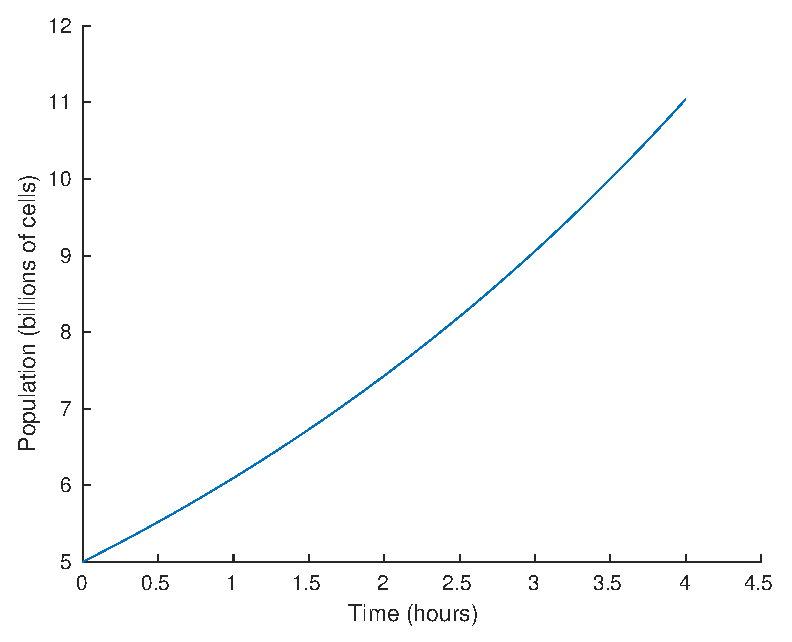
\includegraphics[height=3in]{figs/euler.eps}}
\caption{Solution to a simple differential equation by Euler's method.}
\label{fig:euler}
\end{figure}

The result is a plot of population over time, shown in Figure~\ref{fig:euler}.  The population doubles in a little less than 4 hours.


\section{{\tt ode45}}
\label{sect:ode45}
\index{Differential equations!{\tt ode45}}

A limitation of Euler's method is that it assumes that the derivative is constant between time steps, and that is not generally true.  Fortunately, there are better methods that estimate the derivative between time steps, and they are much more accurate. 

MATLAB provides a function called {\tt ode45} that implements one of these methods.  In this section I'll explain how to use it; you can read more about how it works in Section~\ref{sect:howode45}.

In order to use {\tt ode45}, you have to write a function that evaluates $dy/dt$ as a function of $t$ and $y$.  Fortunately, we already have one, \verb"rate_func":

\begin{code}
function res = rate_func(t, y)
   a = 0.2;
   dydt = a * y;
   res = dydt;
end
\end{code}

We can call {\tt ode45} from the {\sf Command Window} like this:

\begin{code}
[T, Y] = ode45(@rate_func, [0, 4], 5);
plot(T, Y)
\end{code}

The first argument is a function handle, as we saw in Section~\ref{sect:fzero}.  The second argument is the time interval where we want to evaluate the solution; in this case the interval is from $t=0$ to $t=4$ hours.  The third argument is the initial population, 5 billion cells.

{\tt ode45} is the first function we have seen that returns {\em two} output variables.  In order to store them, we have to assign them to two variables, {\tt T} and {\tt Y}.

\begin{figure}
\centerline{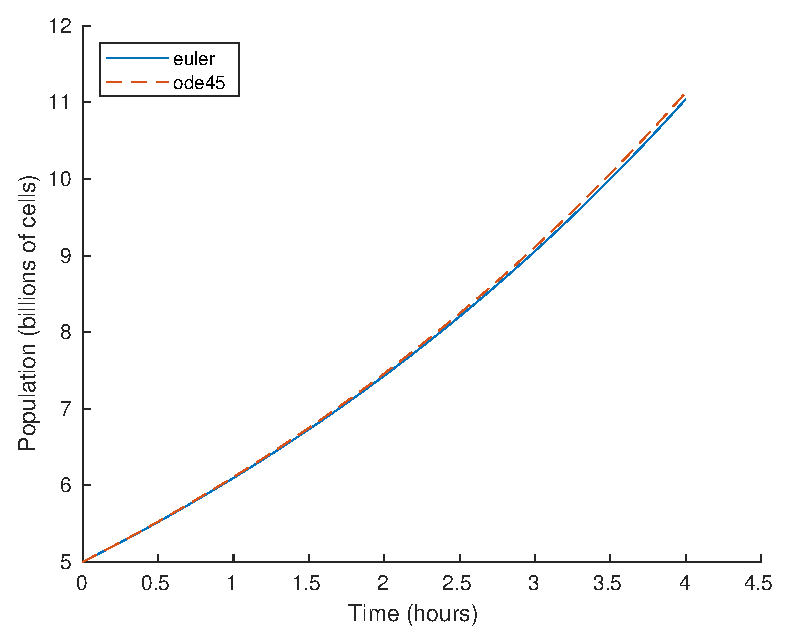
\includegraphics[height=3in]{figs/runge.eps}}
\caption{Solutions to a simple differential equation by Euler's method and {\tt ode45}.}
\label{fig:runge}
\end{figure}

Figure~\ref{fig:runge} shows the results.  The solid line is the estimate we computed with Euler's method; the dashed line is the solution from {\tt ode45}.

For the first 4-5 hours, the two solutions are indistinguishable.  But as the rate of growth increases, Euler's method gets less accurate.

In general, you should use {\tt ode45} instead of Euler's method.  It is almost always more accurate.  


\section{Time dependence}

Looking at \verb"rate_func" in the previous section, you might notice that it takes {\tt t} as an input variables but doesn't use it.  That's because the growth rate does not depend on time; that's because bacteria don't know what time it is.

But rats do.  Or, at least, they know what season it is.
Suppose that the population growth rate for rats
depends on the current population and the availability of food,
which varies over the course of the year.
The differential equation might be something like
%
\begin{equation}
\frac{dy}{dt}(t) = a y(t) \left(1 - \cos (\omega t) \right)
\end{equation}
%
where $t$ is time in days and $y(t)$ is the population at time $t$.

$a$ and $\omega$ are {\bf parameters}.  A parameter is a value that
quantifies a physical aspect of the scenario being modeled.  Parameters are often constants, but in some models they vary in time.

In this example, $a$ characterizes the peak reproductive rate per day, and
$\omega$ is the frequency of a periodic function that describes
the effect of varying food supply on reproduction.

We'll use the values $a = 0.002$
and $\omega = 2 \pi/365$ (one cycle per year).
The growth rate is lowest at $t=0$, on January 1, and highest at $t=365/2$, on June 1.

Now we can write a function that evaluates the growth rate:

\begin{code}
function res = rate_func(t, y)
    a = 0.002;
    omega = 2*pi / 365;
    res = a * y * (1 - cos(omega * t));
end
\end{code}

To test this function, I put it in a file called {\tt rats.m} with a top-level function called {\tt rats}:

\begin{code}
function res = rats()
    t = 31;
    y = 2000;
    res = rate_func(t, y);
end
\end{code}

Suppose there are 2000 rats at $t=31$.  We can compute the growth rate like this:

\begin{code}
>> r = rats

r = 0.5562
\end{code}

So if there are 2000 rats on January 31, we expect them to 
reproduce at a rate that would produce about one new rat every two days. 

Since the growth rate is constantly changing, it is not easy to predict
the future rat population, but that is exactly what {\tt ode45} does.
Here's how:

\begin{code}
[T, Y] = ode45(@rate_func, [0, 365], 2000)
plot(T, Y)
\end{code}

The first argument is a function handle, again.  The second argument is the interval we are interested
in, in this case starting at time 0 and going for 365 days (about a year).  
The third argument is the population at the beginning of the interval, 
in our case $y(0) = 2000$.

\begin{figure}
\centerline{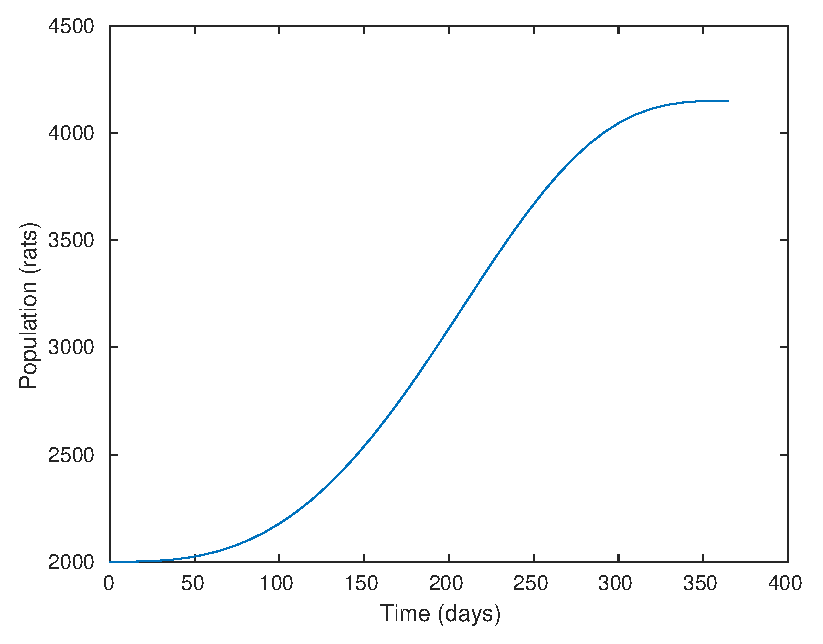
\includegraphics[height=3in]{figs/rats.eps}}
\caption{Solutions to a simple differential equation by Euler's method and {\tt ode45}.}
\label{fig:rats}
\end{figure}

Figure~\ref{fig:rats} shows the results.  The population grows slowly during the winter, quickly during the summer, and the slowly again in the fall.

To see the population at the end of the interval, 
you can display the last element from each vector:

\begin{code}
Y(end)
4.1502e+03
\end{code}

{\tt end} is a special word in MATLAB; when it appears as an index,
it means ``the index of the last element''.  You can use it in an
expression, so {\tt Y(end-1)} is the second-to-last element of
{\tt Y}.


\section{What could go wrong?}

Don't forget the {\tt @} on the function handle.
If you leave it out, MATLAB treats the first argument as a function
call, and calls \verb"rate_func" without providing arguments.

\begin{code}
Not enough input arguments.

Error in rats>rate_func (line 18)
    res = a * y * (1 - cos(omega * t));

Error in rats (line 6)
    [T, Y] = ode45(rate_func, [0, 365], 2000);
\end{code}

Also, remember that the function you write will be called by
{\tt ode45}, which means has to take two input variables, 
{\tt t} and {\tt y}, in that order, and return one output variable, 
{\tt r}.

If you are working with a rate function like this:

\begin{equation}
\frac{dy}{dt}(t) = a y(t)
\end{equation}

You might be tempted to write this:

\begin{code}
function res = rate_func(y)        % WRONG
    a = 0.02;
    res = a * y;
end
\end{code}

But that would be wrong.  So very wrong.  Why?  Because
when {\tt ode45} calls {\tt rate\_func}, it provides two arguments.
If you only take one input variable, you'll get an error.  So
you have to write a function that takes {\tt t} as an input
variable, even if you don't use it.

\begin{code}
function res = rate_func(t, y)     % RIGHT
    a = 0.02;
    res = a * y;
end
\end{code}

Another common error is to write a function that doesn't make
an assignment to the output variable.  If you write something
like this:

\begin{code}
function res = rate_func(t, y)
    a = 0.02;
    omega = 2*pi / 365;
    r = a * y * (1 - cos(omega * t));    % WRONG
end
\end{code}

And then call it from {\tt ode45}, you get

\begin{code}
Output argument "res" (and maybe others) not assigned during call
to "rate_func".
\end{code}

I hope these warnings save you some time debugging.


\section{Labeling axes}

The plots in this chapter have labels on the axes, and one of them has a legend, but I didn't show you how to do that.

The functions to label the axes are {\tt xlabel} and {\tt ylabel}:

\begin{code}
xlabel('Time (hours)')
ylabel('Population (billions of cells)')
\end{code}

The function to generate a legend is {\tt legend}:

\begin{code}
legend('euler', 'ode45')
\end{code}

The arguments are the labels for the lines, in the order they were drawn.  Usually the legend is in the upper right corner, but you can move it by providing an optional argument called {\tt Location}:

\begin{code}
legend('euler', 'ode45', 'Location', 'northwest')
\end{code}

Finally, I saved the figures using {\tt saveas}:

\begin{code}
saveas(gcf, 'runge.eps', 'epsc')
\end{code}

The first argument is the figure we want to save; {\tt gcf}, is a MATLAB command that stands for ``get current figure'', which is the figure we just drew.  The second argument is the filename.  The extension specifies the format we want, which is Encapulated PostScript.  The third argument tells MATLAB what ``driver'' to use.  The details aren't important, but {\tt epsc} generates figures in color.




\section{Glossary}

\begin{description}

\item[differential equation (DE):] An equation that relates the
derivatives of an unknown function.

\item[ordinary DE (ODE):] A DE in which all derivatives are taken with
respect to the same variable.

\item[partial DE:] A DE that includes derivatives with respect to
more than one variable

\item[first order DE:] A DE that includes only first derivatives.

\item[linear DE:] A DE that includes no products or powers of the
function and its derivatives.

\item[time step:] The interval in time between successive estimates
in the numerical solution of a DE.

\item[adaptive:] A method that adjusts the time step to control error.

\item[parameter:] A value that appears in a model to quantify some
physical aspect of the scenario being modeled.

\end{description}

\section{Exercises}

\begin{ex}
Suppose that you are given an 8 ounce cup of coffee at \SI{90}{\celsius}.
You have learned from bitter experience that the hottest coffee you
can drink comfortably is \SI{60}{\celsius}.  

If the temperature of the coffee drops by \SI{0.7}{\celsius} during the first minute, how long will you have to wait to drink your coffee?

You can answer this question with Newton's Law of Cooling\footnote{See \url{https://en.wikipedia.org/wiki/Newton's_law_of_cooling}.}:
%
\begin{equation*}
\frac{dy}{dt}(t) = -k (y(t) - e)
\end{equation*}
%
where $y(t)$ is the temperature of the coffee at time $t$,
$e$ is the temperature of the environment, and $k$ is a parameter
that characterizes the rate of heat transfer from the coffee from the environment.

Let's assume that $e$ is \SI{20}{\celsius} and constant; that is, the coffee does not warm up the room.

Let's also assume $k$ is constant.  In that case, we can estimate it based on the information we have.  If the temperature drops \SI{0.5}{\celsius} during the first minute, when the coffee is \SI{90}{\celsius}, we can write
%
\begin{equation*}
-0.7 = -k (90 - 20)
\end{equation*}
%
Solving this equation yields $k = 0.01$.

Here are some suggestions for getting started:

\begin{itemize}

\item Create a file named {\tt coffee.m} and write a function
called {\tt coffee} that takes no input variables.  Put a simple statement like {\tt x=5} in the body of the function and invoke {\tt coffee} from the {\sf Command Window}.

\item Add a function called {\tt rate\_func} that takes {\tt t} and {\tt y} and computes $\frac{dy}{dt}$.  In this case {\tt rate\_func} does not actually depend on $t$; nevertheless, your function has to take $t$ as
the first input variable in order to work with {\tt ode45}.

\item Test your function by adding a line like {\tt rate\_func(0,90)}
to {\tt coffee}, then call {\tt coffee} from the {\sf Command Window}.
Confirm that the initial rate is \SI{-0.7}{\celsius \per \minute}.

\item Once you get {\tt rate\_func} working, modify
{\tt coffee} to use {\tt ode45} to compute the temperature
of the coffee for 60 minutes.  Confirm that
the coffee cools quickly at first, then more slowly, and reaches
room temperature after about an hour.

\item Plot the results and estimate the time when the temperature reaches \SI{60}{\celsius}.

\end{itemize}

\end{ex}


% chap09
\chapter{Systems of ODEs}

In the previous chapter we used Euler's method and {\tt ode45} to solve a single first-order differential equation.  In this chapter we'll move on to systems of ODEs and implement a model of a predator-prey system.  But first, we have to learn about matrices.


\section{Matrices}

A matrix is a two-dimensional version of a vector.  Like a vector,
it contains elements that are identified by indices.  The difference
is that the elements are arranged in rows and columns, so it takes
{\em two} indices to identify an element.

One of many ways to create a matrix is the {\tt magic} function,
which returns a ``magic square'' with the given size 
\footnote{See \url{https://en.wikipedia.org/wiki/Magic_square}.}:

\index{magic square}

\begin{code}
>> M = magic(3)

M =  8     1     6
     3     5     7
     4     9     2
\end{code}

If you don't know the size of a matrix, you can use {\tt whos} to
display it:

\begin{code}
>> whos
  Name        Size                    Bytes  Class
  M           3x3                        72  double array
\end{code}

Or the {\tt size} function, which returns a vector:

\index{Matrices!{\tt size}}

\begin{code}
>> V = size(M)

V = 3     3
\end{code}

The first element is the number of rows, the second is the number of
columns.

To read an element of a matrix, you specify the row and column numbers:

\begin{code}
>> M(1,2)

ans = 1

>> M(2,1)

ans = 3
\end{code}

When you are working with matrices, it takes some effort to remember
which index comes first, row or column.  I find it useful to repeat
``row, column'' to myself, like a mantra.  You might also find it
helpful to remember ``down, across,'' or the abbreviation RC.

Another way to create a matrix is to enclose the elements in
brackets, with semi-colons between rows:

\begin{code}
>> D = [1,2,3 ; 4,5,6]

D =  1     2     3
     4     5     6

>> size(D)

ans = 2     3
\end{code}


\section{Row and column vectors}
\label{rowvector}
\index{Matrices!row and column vectors}

Although it is useful to think in terms of scalars, vectors and matrices,
from MATLAB's point of view, everything is a matrix.  A scalar
is just a matrix that happens to have one row and one column:

\begin{code}
>> x = 5;
>> size(x)

ans = 1     1
\end{code}

And a vector is a matrix with only one row:

\begin{code}
>> R = 1:5;
>> size(R)

ans = 1     5
\end{code}

Well, some vectors, anyway.  Actually, there are two kind
of vectors.  The ones we have seen so far are called {\bf row vectors},
because the elements are arranged in a row; the other kind are
{\bf column vectors}, where the elements are in a single column.

One way to create a column vector is to create a matrix with only
one element per row:

\begin{code}
>> C = [1;2;3]

C =

     1
     2
     3

>> size(C)

ans = 3     1
\end{code}

The difference between row and column vectors is important in
linear algebra, but for most basic vector operations, it doesn't matter.  When you index the elements of a vector, you don't have to know what kind
it is:

\begin{code}
>> R(2)

ans = 2

>> C(2)

ans = 2
\end{code}



\section{The transpose operator}
\index{Matrices!transpose}

The transpose operator, which looks remarkably like an apostrophe,
computes the {\bf transpose} of a matrix, which is a new matrix
that has all of the elements of the original, but with each row
transformed into a column (or you can think of it the other way around).

In this example:

\begin{code}
>> D = [1,2,3 ; 4,5,6]

D =  1     2     3
     4     5     6
\end{code}

{\tt D} has two rows, so its transpose has two columns:

\begin{code}
>> Dt = D'

Dt = 1     4
     2     5
     3     6
\end{code}

\begin{ex}
What effect does the transpose operator
have on row vectors, column vectors, and scalars?
\end{ex}


\section{Lotka-Volterra}
\label{sect:lotka}

The Lotka-Volterra model describes the interactions between two
species in an ecosystem, a predator and its prey.  As an example, we'll consider weasels and rabbits.

The model is governed by the following system of differential equations:

\begin{eqnarray}
    \frac{dr}{dt} &=& \alpha r - \beta r w
    \\[6pt]
    \frac{dw}{dt} &=& - \gamma w + \delta r w
\end{eqnarray}
%
where $r$ and $w$ are the populations of rabbits and weasels,
and $\alpha$, $\beta$, $\gamma$, and $\delta$ are parameters
governing the interactions between the two species.\footnote{See
\url{https://en.wikipedia.org/wiki/Lotka-Volterra_equations}.}

At first glance you might think you could solve these equations by
calling {\tt ode45} once to solve for $r$ as a function of time and
once to solve for $w$.  The problem is that each equation involves
both variables, which is what makes this a {\bf system of equations}
and not just a list of unrelated equations.  To solve a system, you
have to solve the equations simultaneously.

\index{Differential equations!systems of equations}

Fortunately, {\tt ode45} can handle systems of equations.  The
difference is that the initial condition is a vector that contains
initial values $r(0)$ and $w(0)$, and the output is a matrix
that contains one column for $r$ and one for $w$.

Here's what the rate function looks like
with the parameters $\alpha = 0.1$, $\beta = 0.01$, $\gamma = 0.1$, 
and $\delta = 0.002$:

\begin{code}
function res = rate_func(t, V)
    % unpack the elements of V
    r = V(1);
    w = V(2);

    % set the parameters
    a = 0.1;  
    b = 0.01;  
    g = 0.1;   
    d = 0.002; 

    % compute the derivatives
    drdt = a*r - b*r*w;
    dwdt = -g*w + d*r*w;

    % pack the derivatives into a vector
    res = [drdt; dwdt];
end
\end{code}

Remember, the first input variable must be the ``time'' variable.
Even though time is not used in this rate function, its presence is required by the {\tt ode45} solver.

The second input variable is a vector with two elements,
$r(t)$ and $w(t)$.  I gave it a capital letter to remind me that it
is a vector.  The body of the function includes four sections,
each explained by a comment.

The first section {\bf unpacks} the vector by copying the elements
into scalar variables.  This isn't necessary, but giving names to
these values helps me remember what's what.  It also makes the third
section, where we compute the derivatives, resemble the mathematical
equations we were given, which helps prevent errors.

The second section sets the parameters that describe the
reproductive rates of rabbits and foxes, and the characteristics of
their interactions.  If we were studying a real system, these values
would come from observations of real animals, but for this example
I chose values that yield interesting results.

The last section {\bf packs} the computed derivatives back into a
vector.  When {\tt ode45} calls this function, it provides a vector
as input and expects to get a vector as output.

Sharp-eyed readers will notice something different about this line:

\begin{code}
    res = [drdt; dwdt];
\end{code}

The semi-colon between the elements of the vector is not an error.  It
is necessary in this case because {\tt ode45} requires the result of
this function to be a column vector.

As always, it is a good idea to test your rate function before you call {\tt ode45}.  I created a file named {\tt lotka.m} with the following top-level function:

\begin{code}
function res = lotka()
    t = 0;
    V_init = [80, 20];
    rate_func(t, V_init)
end
\end{code}

\verb"V_init" is a vector that represents the initial condition, 80 rabbits and 20 weasels.  The result from \verb"rate_func" is:

\begin{code}
-8.0000
 1.2000
 \end{code}
  
Which means that with these initial conditions, we expect the rabbit population to decline initially at a rate of 8 per week, and the weasel population to increase by 1.2 per week.  
  
Now we can run {\tt ode45} like this:

\begin{code}
tspan = [0, 200]
[T, M] = ode45(@rate_func, tspan, V_init)
\end{code}

The first argument is the function handle for the rate function.
The second argument is the time span, from 0 to 200 weeks.
The third argument is the initial condition.


\section{Output matrices}

{\tt ode45} returns two values: {\tt T}, which is a vector of time values, and {\tt M}, which is a matrix with one column for each
population and one row for each time value in {\tt T}.

\begin{code}
>> size(M)
ans = 185     2
\end{code}

This organization -- one column per variable -- is a common way to
use matrices.  {\tt plot} understands this organization, so if you
do this:

\begin{code}
>> plot(T, M)
\end{code}

MATLAB understands that it should plot each column from {\tt M}
versus {\tt T}.

You can copy the columns of {\tt M} into other variables like
this:

\begin{code}
>> R = M(:, 1);
>> W = M(:, 2);
\end{code}

In this context, the colon represents the range from 1 to {\tt end},
so {\tt M(:, 1)} means ``all the rows, column 1'' and
{\tt M(:, 2)} means ``all the rows, column 2.''

\begin{code}
>> size(R)
ans = 185     1

>> size(W)
ans = 185     1
\end{code}

So {\tt R} and {\tt W} are column vectors.

Now we can plot these vectors separately, which makes it easier to give them different style strings:

\begin{code}
>> plot(T, R, '-')
>> plot(T, W, '--')
\end{code}

\begin{figure}
\centerline{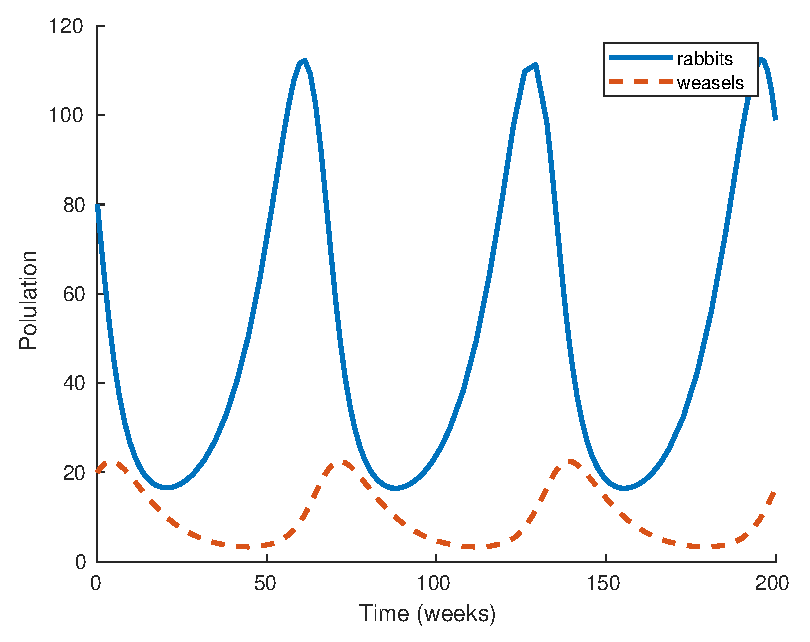
\includegraphics[height=3in]{figs/lotka.eps}}
\caption{Solution for the Lotka-Volterra model.}
\label{fig:lotka}
\end{figure}

Figure~\ref{fig:lotka} shows the results. The x-axis is time in weeks; the y-axis is population.  The top curve shows the population of rabbits; the bottom curve shows weasels.

Initially there are too many weasels, so the rabbit population declines.  Then there are not enough rabbits, and the weasel population declines.  That allows the rabbit population to recover, and the pattern repeats.

This cycle of ``boom and bust'' is typical of the Lotka-Volterra model.

\section{Phase plot}

Instead of plotting the two populations over time, it is sometimes useful to plot them against each other, like this:

\begin{code}
>> plot(R, W)
\end{code}

\begin{figure}
\centerline{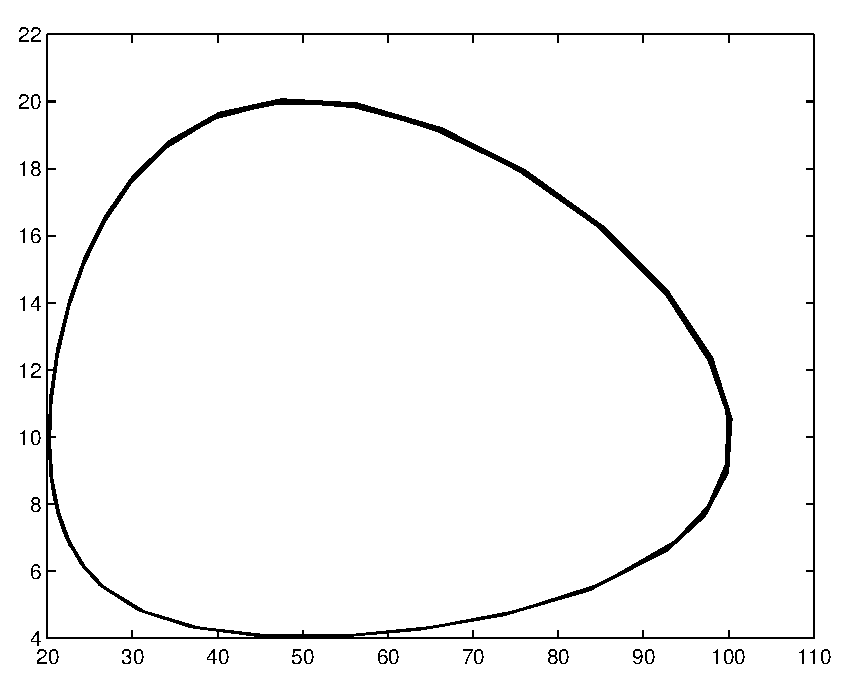
\includegraphics[height=3in]{figs/phase.eps}}
\caption{Phase plot from the Lotka-Volterra model.}
\label{fig:phase}
\end{figure}

Figure~\ref{fig:phase} shows the result.  Each point on this plot represents a certain number of rabbits (on the
x axis) and a certain number of weasels (on the y axis).

Since these are the only two variables in the system, each point in
this plane describes the complete {\bf state} of the system.

\index{phase plot}
\index{trajectory}
\index{state}

Over time, the state moves around the plane; this figure shows
the path traced by the state over time; this path
is called a {\bf trajectory}.

Since the behavior of this system is periodic, the
trajectory is a loop.

If there are 3 variables in the system, we need 3 dimensions to show
the state of the system, so the trajectory is a 3-D curve.
You can use {\tt plot3} to trace trajectories in 3 dimensions,
but for 4 or more variables, you are on your own.


\section{What could go wrong?}

The output vector from the rate function has to be a column vector; otherwise you get an error:

\begin{code}
Error using odearguments (line 93)
RATE_FUNC must return a column vector.

Error in ode45 (line 115)
  odearguments(FcnHandlesUsed, solver_name, ode, tspan, y0, 
               options, varargin);

Error in lotka (line 7)
    [T, M] = ode45(@rate_func, tspan, V_init);
\end{code}

Which is pretty good as error messages go.  It's not clear {\em why}
it needs to be a column vector, but that's not our problem.

Another possible error is reversing the order of the elements in the
initial conditions, or the vectors inside {\tt lotka}.  MATLAB
doesn't know what the elements are supposed to mean, so it can't catch
errors like this; it will just produce incorrect results.

The order of the elements (rabbits and weasels) is up to you, but
you have to be consistent.  That is, the initial conditions you
provide when you call {\tt ode45} have to be the same as the order,
inside \verb"rate_func", where you unpack the input vector and repack
the output vector.



\section{Glossary}

\begin{description}

\item[row vector:] A matrix that has only one row.

\item[column vector:] A matrix that has only one column.

\item[transpose:] An operation that transforms the rows of a matrix
into columns (or the other way around, if you prefer).

\item[system of equations:] A collection of equations written in terms of
the same set of variables.

\item[unpack:] To copy the elements of a vector into a set of variables.

\item[pack:] To copy values from a set of variables into a vector.

\item[state:] If a system can be described by a set of variables,
the values of those variables are called the state of the system.

\item[phase plot:] A plot that shows the state of a system as point
in the space of possible states.

\item[trajectory:] A path in a phase plot that shows how the state of
a system changes over time.


\end{description}

\section{Exercises}

\begin{ex}

Based on the examples we have seen so far, you would think that
all ODEs describe population as
a function of time, but that's not true.

According to Wikipedia,
``The Lorenz attractor, introduced by Edward Lorenz in 1963, is a
non-linear three-dimensional deterministic dynamical system derived
from the simplified equations of convection rolls arising in the
dynamical equations of the atmosphere. For a certain set of parameters
the system exhibits chaotic behavior and displays what is today called
a strange attractor...''\footnote{See \url{https://en.wikipedia.org/wiki/Lorenz_attractor}.}

The system is described by this system of differential equations:
%
\begin{eqnarray}
x_t &=& \sigma (y - x)  \\
y_t &=& x (r - z) - y   \\
z_t &=& xy - b z
\end{eqnarray}
%
Common values for the parameters are $\sigma = 10$, $b = 8/3$, and $r=28$.

Use {\tt ode45} to estimate a solution to this
system of equations.


\begin{enumerate}

\item Create a file named {\tt lorentz.m} with a top-level function named {\tt lorenz} and a helper function named \verb"rate_func".

\item  The rate function should
takes {\tt t} and {\tt V} as input variables, where the components
of {\tt V} are understood to be the current values of {\tt x},
{\tt y} and {\tt z}.  It should compute the corresponding derivatives
and return them in a single column vector.

\item Test the function by calling it from the top-level function with values like $t=0$, $x=1$, $y=2$, and $z=3$.  Once you get your function working, you should make it a silent function before calling {\tt ode45}.

\item Use {\tt ode45}
to estimate the solution for the time span $[0, 30]$
with the initial condition $x=1$, $y=2$, and $z=3$.

\item Plot the results as a time series, that is, each of the variables as a function of time.

\item Use {\tt plot3} to plot the trajectory of
$x$, $y$, and $z$.

\end{enumerate}

% lorenz.m
\end{ex}


% chap10
\chapter{Second-order Systems}

So far we have seen first-order differential equations and systems of first-order ODEs.  In this chapter we introduce second-order systems, which are particularly useful for modeling Newtonian motion.


\section{Newtonian motion}

Newton's second law of motion is often written like this:

\begin{equation}
    F = m a
\end{equation}

where $F$ is the net force acting on an object, $m$ is the
mass of the object, and $a$ is the acceleration of the object.

This equation suggests
that if you know $m$ and $a$ you can compute force, which is true,
but in most physical simulations it is the other way around:  based on a
physical model, you know $F$ and $m$, and you compute $a$.

So if we know acceleration as a function of time, how do we
find the position of the object, $r$?  Well, we know that acceleration
is the second derivative of position, so we can write a differential
equation

\begin{equation}
\label{eq:pos_acc}
    \frac{d^2r}{dt^2} = a
\end{equation}

where $\frac{d^2r}{dt^2}$ is the second time derivative of $r$.

Because this equation includes a second derivative, it is
a second-order ODE.  {\tt ode45} can't solve the equation this form, but
by introducing a new variable, {\tt v}, for velocity, we can rewrite it
as a system of first-order ODEs:

\begin{eqnarray}
    \label{eq:pos_vel}
    \frac{dr}{dt} &=& v   \\
    \label{eq:vel_acc}
    \frac{dv}{dt} &=& a   \\
\end{eqnarray}

The first equation says that the first derivative of $r$ is $v$;
the second equation says that the first derivative of $v$ is $a$.


\section{Freefall}
\label{sect:freefall}

As an example, let's get back to the question from Exercise~\ref{penny}:

\begin{quote}
If you drop a penny from the top of the Empire State Building, how long does it take to reach the sidewalk, and how fast it is going when it gets there?
\end{quote}

We'll start with no air resistance; then we'll add air resistance to the model and see what effect it has.

Near the surface of the earth,
acceleration due to gravity is $-9.8$ $m/s^2$, where the minus sign
indicates that gravity pulls down.

If the object falls straight down, we can describe its position with a
scalar value $y$, representing altitude.

Here is a rate function we can use with {\tt ode45} to solve
this problem:

\begin{code}
function res = rate_func(t, X)
    % unpack position and velocity
    y = X(1);      
    v = X(2);      
    
    % compute the derivatives
    dydt = v;
    dvdt = -9.8;

    % pack the derivatives into a column vector
    res = [dydt; dvdt];
end
\end{code}

The rate function takes {\tt t} and {\tt X} as input variables, where the elements of {\tt X} are understood to be the position and velocity of the object.
It returns a column vector that contains {\tt dydt} and {\tt dvdt}, which
are velocity and acceleration, respectively.

Since velocity is the second element of {\tt X}, we can simply assign this value to {\tt dydt}.
And since the derivative of velocity is acceleration, we can assign the acceleration of gravity to {\tt dvdt}.

As always, we should test the rate function before we call {\tt ode45}.  Here's the top-level function we can use to test it:

\begin{code}
function penny()
   t = 0;
   X = [381, 0];
   rate_func(t, X)
end
\end{code}

The initial condition of {\tt X} is the initial position, which is the height of the Empire State Building, about \SI{381}{\meter}, and the initial velocity, which is \SI{0}{\meter \per \second}.

The result from \verb"rate_func" is:

\begin{code}
    0
   -9.8000
\end{code}

which is what we expect.

Now we can run {\tt ode45} with this rate function:

\begin{code}
tspan = [0, 10]
[T, M] = ode45(@rate_func, tspan, X)
\end{code}

As always, the first argument is the function handle, the second
is the time span (30 seconds) and the third is the initial
condition.

The result is a vector, {\tt T}, that contains the time values, and a matrix, {\tt M}, that contains two columns, one for altitude and one for velocity.

We can extract the first column and plot it, like this:

\begin{code}
Y = M(:, 1)
plot(T, Y)
\end{code}


\begin{figure}
\centerline{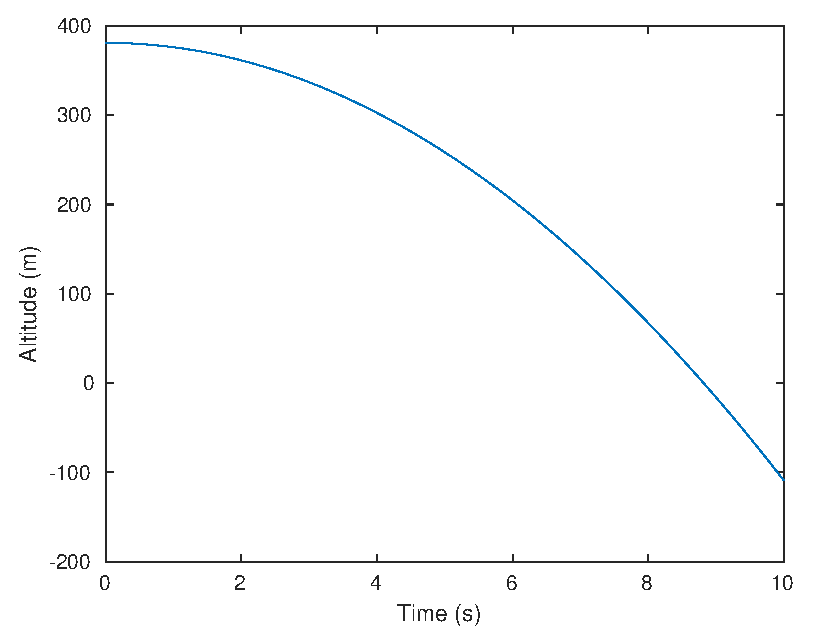
\includegraphics[height=3in]{figs/penny.eps}}
\caption{Altitude versus time for an object in free fall.}
\label{fig:penny}
\end{figure}

Figure~\ref{fig:penny} shows the result.  Altitude drops slowly at first and picks up speed.  Between 8 and 9 seconds, the altitude reaches 0, which means the penny hits the sidewalk.  But {\tt ode45} doesn't know where the ground is, so the penny keeps going through zero into negative altitude.  We can solve that problem using events.


\section{ODE events}
\label{sect:events}

\index{ODE events}

%Normally when you call {\tt ode45} you specify a start time and
an end time.  But sometimes you don't know ahead of time when the
simulation should end.  MATLAB provides a way to deal with this problem; here's how it works:

\begin{enumerate}

\item Define an {\bf event function} that specifies when the simulation should stop.  For example,  here is an event function for the penny example:

\begin{code}
function [value, isterminal, direction] = event_func(t,X)
    value = X(1);
    isterminal = 1;
    direction = -1;
end
\end{code}

The event function takes the the same input variables as the rate function and returns three output variables: {\tt value} determines whether an {\bf event} can occur, {\tt direction} determines whether it does, and {\tt isterminal} determines what happens.

An event can occur when {\tt value} passes through 0.
If {\tt direction} is positive, the event only occurs if {\tt value} is increasing.
If {\tt direction} is negative, the event only occurs if {\tt value} is decreasing.
If {\tt direction} is 0, the event always occurs.

If {\tt isterminal} is 1, the event causes the simulation to end; otherwise the simulation continues.

This event function uses the altitude of the penny as {\tt value}, so an event occurs when the altitude is decreasing and passes through 0.  When it does, the simulation ends.

\item Use {\tt odeset} to create an object called {\tt options}:

\begin{code}
options = odeset('Events', @event_func);
\end{code}
%
The name of the option is {\tt Events} and the value is the handle of the event function.  

\item Pass {\tt options} as a fourth argument to {\tt ode45}:

\begin{code}
[T, M] = ode45(@rate_func, tspan, X, options);
\end{code}

When {\tt ode45} runs, it invokes \verb"event_func" after each timestep.  If the event function indicates that a terminal event occurred, 
{\tt ode45} stop the simulation.

\end{enumerate}

Let's look at the results from the penny example.  

\begin{code}
>> T(end)
8.8179

>> M(end, :)
0.0000  -86.4153
\end{code}

The last value of {\tt T} is 8.817, which is the number of seconds the penny takes to reach the sidewalk.

The last row of {\tt M} indicates that the final altitude is 0, which is what we wanted, and the final velocity is about \SI{86}{\meter \per \second}.


\section{Air resistance}
\label{sect:air_resistance}

To make this simulation more realistic, we can add air resistance.
For sizable objects moving relatively quickly through air, the force due to air resistance, called ``drag'', is proportional to velocity squared.  
For an object falling down, drag is
directed up, so if velocity is negative, drag force is positive.

\begin{equation}\label{eq:simpledrag}
    f_{d} = -sgn(v) b v^2 
\end{equation}

where $v$ is velocity and
$b$ is a drag constant that depends on the density of
air, the cross-sectional area of the object and the shape
of the object.  

% b is used in the book "Physics for Scientists and Engineers" by Paul A. Tipler.

$sgn$ is the sign or signum function, which is 1 for positive values of 
$v$ and -1 for negative values.  So $f_d$ is always in the opposite direction of $v$.

To convert from force to acceleration, we have to know mass, but that's easy to find: the mass of a penny is about \SI{2.5}{\gram}.  It's not as easy to find the drag constant, but I have estimated\footnote{Based on reports that the terminal velocity of a penny is about \SI{18}{\meter \per \second}.} that it is about \SI{75e-6}{\kilogram \per \meter}.

Here's a function that takes {\tt t} and {\tt X} as input variables and returns the total acceleration of the penny due to gravity and drag:

\begin{code}
function res = acceleration(t, X)
    b = 75e-6;                % drag constant in kg/m
    v = X(2);                 % velocity in m/s
    f_d = -sign(v) * b * v^2; % drag force in N

    m = 2.5e-3;               % mass in kg
    a_d = f_d / m;            % drag acceleration in m/s^2

    a_g = -9.8;               % acceleration due to gravity in m/s^2
    res = a_g + a_d;          % total acceleration
end
\end{code}

The first three lines compute force due to drag.
The next two lines compute acceleration due to drag.
The last two lines compute total acceleration due to drag and gravity.

Be careful when you are working with forces and accelerations; make sure
you only add forces to forces or accelerations to accelerations.  In my
code, I use comments to remind myself what units the values are in.
That helps me avoid nonsense like adding forces to accelerations.

To use this function, I made a small change in \verb"rate_func":

\begin{code}
function res = rate_func(t, X)
    y = X(1);      
    v = X(2);      
    
    dydt = v;
    dvdt = acceleration(t, X);   % this line has changed

    res = [dydt; dvdt];
end

\end{code}

\begin{figure}
\centerline{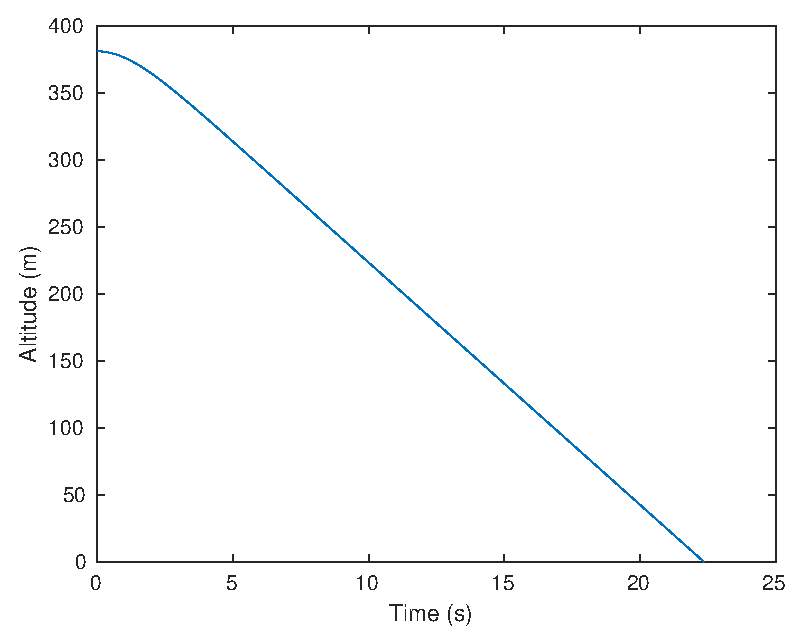
\includegraphics[height=3in]{figs/penny2.eps}}
\caption{Altitude versus time for an penny in free fall with air resistance.}
\label{fig:penny2}
\end{figure}

Everything else is the same.
Figure~\ref{fig:penny2} shows the result. 

Air resistance makes a big difference!  Velocity increases until
the drag acceleration equals $g$; after that, velocity is constant and position decreases linearly (and much more slowly than it would in a vacuum). 

With air resistance, the time until the penny hits the sidewalk is \SI{22.4}{\second}, substantially longer than before (\SI{8.8}{\second}).

And the final velocity is \SI{18.1}{\meter \per \second}, substantially slower than before (\SI{86}{\meter \per \second}).


%\section{Glossary}
%
%\begin{description}
%
%\item[ODE event:]
%
%\item[event function:]
%
%\end{description}


\section{Exercises}


\begin{ex}
The drag constant for a skydiver without a parachute is about \SI{0.2}{\kilogram \meter}.  Modify the penny code from this chapter to simulate the descent of a \SI{75}{\kilogram} skydiver from an initial altitude of \SI{4000}{\meter}.  What is the velocity of the skydiver on impact?

After opening a parachute, the velocity of the skydiver slows to about \SI{5}{\meter\per\second}.  Use your simulation to find the drag constant that yields a terminal velocity of \SI{5}{\meter\per\second}.

Increase the mass of the skydiver, and confirm that terminal velocity increases.  This phenomenon is the source of the intuition that heavy objects fall faster; in air, they do!

Now suppose the skydiver free falls until they get to altitude \SI{1000}{\meter} before opening the parachute.  How long would it take them to reach the ground?

What is the lowest altitude where the skydiver can open the parachute and still land at less than \SI{6}{\meter\per\second} (assuming that the parachute opens and deploys instantly)?

% skydiver.m
\end{ex}



\begin{ex}
\label{ex:earth}

Here's a question from the web site {\em Ask an Astronomer}\footnote{\url{https://web.archive.org/web/20180617133223/http://curious.astro.cornell.edu/about-us/39-our-solar-system/the-earth/other-catastrophes/57-how-long-would-it-take-the-earth-to-fall-into-the-sun-intermediate}}:

\begin{quote}
``If the Earth suddenly stopped orbiting the Sun, I know eventually it would be pulled in by the Sun's gravity and hit it. How long would it take the Earth to hit the Sun? I imagine it would go slowly at first and then pick up speed.''
\end{quote}

Use {\tt ode45} to answer this question.  Here are some suggestions about how to proceed:

\begin{enumerate}

\item Look up the Law of Universal Gravitation and any constants you need. I suggest you work entirely in SI units: meters, kilograms, and Newtons.

\item When the distance between the Earth and the Sun gets small, this system behaves badly, so you should use an event function to stop when the surface of Earth reaches the surface of the Sun.

\item Express your answer in days, and plot the results as millions of kilometers versus days.

\end{enumerate}

% earth.m
\end{ex}


% chpt11
\chapter{Two dimensions}

\section{Spatial vectors}
\label{sect:spacial}

The word ``vector'' means different
things to different people.  In MATLAB, a vector is a matrix that has
either one row or one column.  So far we have used MATLAB vectors to
represent:

\begin{description}

\item[sequences:] A sequence is a set of values identified by
integer indices; it is natural to store the elements of the
sequence as elements of a MATLAB vector.

\item[state vectors:] A state vector is a set of values that
describes the state of a physical system.  When you call
{\tt ode45}, you give it initial conditions in a state
vector.  Then when {\tt ode45} calls your rate function, it
gives you a state vector.

\item[time series:] The results from {\tt ode45} are vectors, {\tt T} and {\tt Y}, that represent a time series, that is, a mapping from the time values in {\tt T} to the values in {\tt Y}.

\end{description}

In this chapter we will see another use of MATLAB vectors: representing
{\bf spatial vectors}.  A spatial vector represents a multidimensional physical quantity like position, velocity, acceleration, or force.

\index{Spatial vectors!coordinate representation}

For example, to represent a position in two-dimensional space, we can use a vector with two elements:

\begin{code}
>> P = [3 4]
\end{code}

To interpret this vector, we have to know what coordinate system it is defined in.  Most commonly, we use a Cartesian system where the x-axis points east and the y-axis points north.  In that case {\tt P} represents a point 3 units east and 4 units north of the origin.

Spatial vector represent the magnitude and direction of a physical quantity.  For example, the magnitude of {\tt P} is the distance from the origin to {\tt P}, which is the hypotenuse of the triangle with sides 3 and 4.  We can compute it using the Pythagorean theorem:

\begin{code}
>> sqrt(sum(P.*P))
ans = 5
\end{code}

Or more simply by using the function {\tt norm}, which computes the
``Euclidean norm'' of a vector, which is its magnitude:

\begin{code}
>> norm(P)
ans = 5
\end{code}

There are two ways to get the direction of a vector.  One convention is to compute the angle between the vector and the x-axis:

\begin{code}
>> atan2(P(2), P(1))
ans = 0.9273
\end{code}

In this example, the angle is about \SI{0.9}{\radian}.  But for computational purposes, we often represent direction with a {\bf unit vector}, which is a vector with length 1.  To get a unit vector we can divide a vector by its length:

\begin{code}
function res = hat(V)
    res = V / norm(V)
end
\end{code}
 
This function takes a vector, {\tt V}, and returns a unit vector with the same direction as {\tt V}.  It is called {\tt hat} because in mathematical notation, unit vectors are written with a ``hat'' symbol.  
For example, the unit vector with the same direction as $\vec{P}$ would be written $\uvec{P}$. 


\section{Adding vectors}

Vectors are particularly useful for representing quantities like force and acceleration because we can add them up without having to think explicitly about direction.

As an example, suppose we have two vectors representing forces:

\begin{code}
>> A = [2, 4];
>> B = [2, -2];
\end{code}

{\tt A} represents a force pulling northeast; {\tt B} represents a force pulling southeast, as shown in Figure~\ref{fig:vector2}

\begin{figure}
\centerline{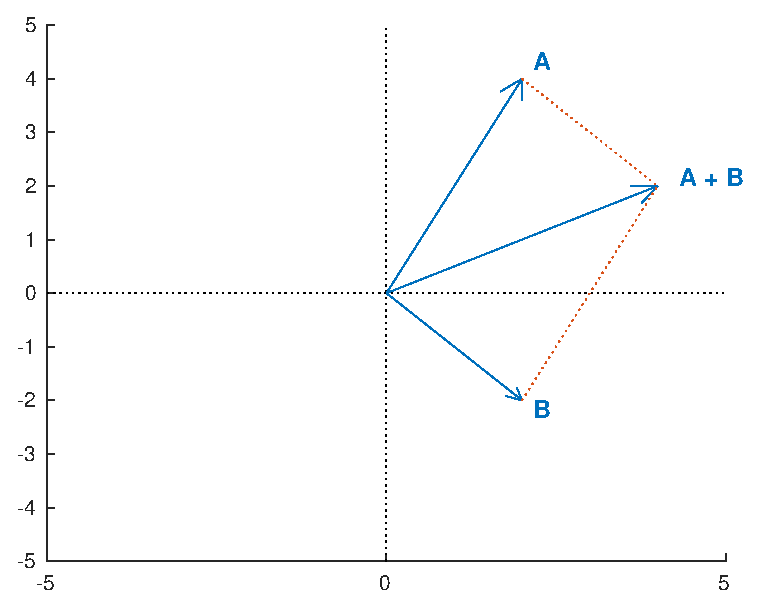
\includegraphics[height=3in]{figs/vector2.eps}}
\caption{The sum of two forces represented by vectors.}
\label{fig:vector2}
\end{figure}

To compute the sum of these forces, all we have to do is add the vectors:

\begin{code}
>> A + B
ans = 4     2
\end{code}

This will come in handy later in the chapter.


\section{ODEs in two dimensions}
\label{sect:projectile}

So far we have used {\tt ode45} to solve a system of first-order equations and a single second-order equation.  Now we'll take one more step, solving a system of second-order equations.

As an example, we'll simulate the flight of a baseball.
Assuming there is no wind and no spin on the ball, it should travel in a vertical plane, so we can think of the system as
two-dimensional, with $x$ representing the horizontal distance
traveled and $y$ representing height or altitude.

Here's a rate function we can use to simulate this system with {\tt ode45}:

\begin{code}
function res = rate_func(t, W)
    P = W(1:2);
    V = W(3:4);

    dPdt = V;
    dVdt = acceleration(t, P, V);

    res = [dPdt; dVdt];
end

function res = acceleration(t, P, V)
    g = 9.8;             % acceleration of gravity in m/s^2
    a_gravity = [0; -g];
    res = a_gravity;
end
\end{code}

The second argument of \verb"rate_func" is understood to be a vector,
{\tt W}, with four elements.  The first two are assigned to {\tt P},
which represents position; the last two are assigned to {\tt V}, which
represents velocity. Both {\tt P} and {\tt V} have two elements
representing the $x$ and $y$ components.

The goal of the rate function is to compute the derivative of {\tt W}, so the output has to be a vector with four elements, where the first two represent the derivative of {\tt P}  and the last two represent the derivative of {\tt V}.

The derivative of {\tt P} is velocity.  We don't have to compute it; we were given it as part of {\tt W}.

The derivative of {\tt V} is acceleration.  To compute it, we call {\tt acceleration}, which takes as input variables time, position and velocity.  In this example, we don't use any of the input variables, but we will soon.

For now we'll ignore air resistance, so the only force on the baseball is gravity.  We represent acceleration due to gravity with a vector that has magnitude {\tt g} and direction along the negative $y$ axis.

Let's assume that a ball is batted from an initial position \SI{1}{\meter} above home plate, with an initial velocity of \SI{30}{\meter\per\second} in the horizontal and \SI{40}{\meter\per\second} in the vertical direction.

Here's how we can call {\tt ode45} with these initial conditions:
 
\begin{code}
    P = [0; 3];       % initial position in m
    V = [40; 30];     % initial velocity in m/s
    W = [P; V];       % initial condition
    
    tspan = [0 8]
    [T, M] = ode45(@rate_func, tspan, W);
\end{code}

{\tt P} and {\tt V} are column vectors because we put semi-colons between the elements.  So {\tt W} is a column vector with four elements.
{\tt tspan} specifies that we want to run the simulation for \SI{6}{\second}.

The output variables from {\tt ode45} are a vector, 
{\tt T}, that contains time values and a matrix, {\tt M}, with four columns: the first two are position; the last two are velocity.

Here's how we can plot position as a function of time:

\begin{code}
	X = M(:, 1);
    Y = M(:, 2);
    
    plot(T, X)
    plot(T, Y)
\end{code}

{\tt X} and {\tt Y} get the first and second columns from {\tt M}, which are the $x$ and $y$ coordinates of position.

\begin{figure}
\centerline{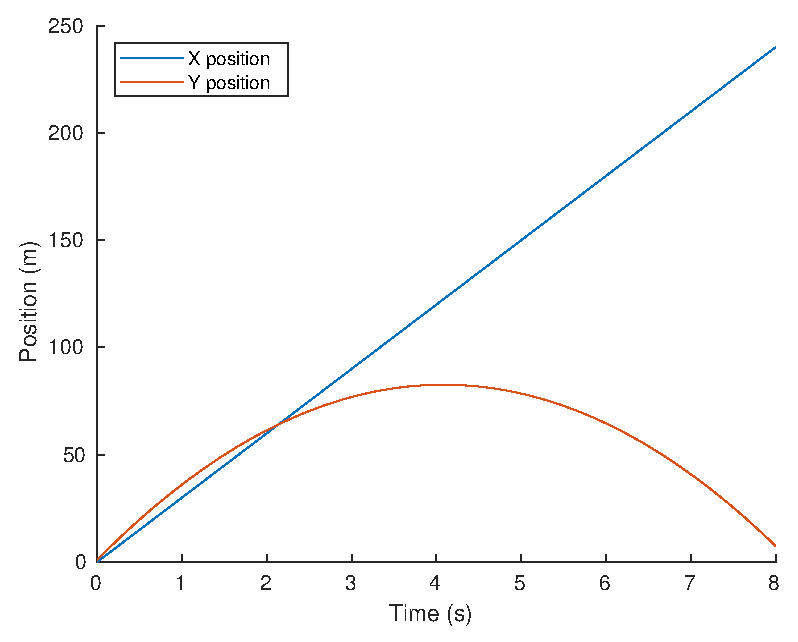
\includegraphics[height=3in]{figs/baseball1.eps}}
\caption{Simulated flight of a baseball neglecting drag force.}
\label{fig:baseball1}
\end{figure}

Figure~\ref{fig:baseball1} shows what they look like.  The $x$ coordinate increases linearly because the $x$ velocity is constant.  The $y$ coordinate goes up and down, as we expect.

The simulation ends just before the ball lands, having traveled almost \SI{250}{\meter}.  That's substantially farther than a real baseball would travel, because we have ignored air resistance, or ``drag force''.


\section{Drag force}
\label{sect:drag}

A simple model for the drag force on a baseball is:

\begin{equation}
    \vec{F_d} = - \frac{1}{2} ~ \rho v^2 C_d A \uvec{V}
\end{equation}

where $\vec{F_d}$ is a vector that represents the force on the baseball
due to drag, 
$\rho$ is the density of air, 
$C_d$ is the drag coefficient, and
$A$ is the cross-sectional area .

$\vec{V}$ is the baseball's velocity vector; $v$ is the magnitude of $V$ and $\uvec{V}$ is a unit vector in the same direction as $V$.  The minus sign at the beginning means that the result is in the opposite direction as $V$.

The following function computes the drag force on a baseball:

\begin{code}
 function res = drag_force(V)
    C_d = 0.3;      % dimensionless
    rho = 1.3;      % kg / m^3
    A = 0.0042;     % m^2
    v = norm(V);    % m/s

    res = - 1/2 * C * rho * A * v * V;
end
\end{code}
  
The drag coefficient for a baseball is about 0.3.  
The density of air at sea level is about \SI{1.3}{\kilogram\per\meter\cubed}.
The cross-sectional area of a baseball is \SI{0.0042}{\meter\squared}.

Now we have to update {\tt acceleration} to take drag into account:

\begin{code}
function res = acceleration(t, P, V)
    g = 9.8;                       % acceleration of gravity in m/s^2
    a_gravity = [0; -g];

    m = 0.145;                     % mass in kilograms
    a_drag = drag_force(V) / m;
    res = a_gravity + a_drag;
end
\end{code}

As in Section~\ref{sect:projectile}, {\tt acceleration} represents acceleration due to gravity with a vector that has magnitude {\tt g} and direction along the negative $y$ axis.
But now it also computes drag force, then divides by the mass of the baseball to get acceleration due to drag.
Finally, it adds \verb"a_gravity" and \verb"a_drag" to get the total acceleration of the baseball.

\begin{figure}
\centerline{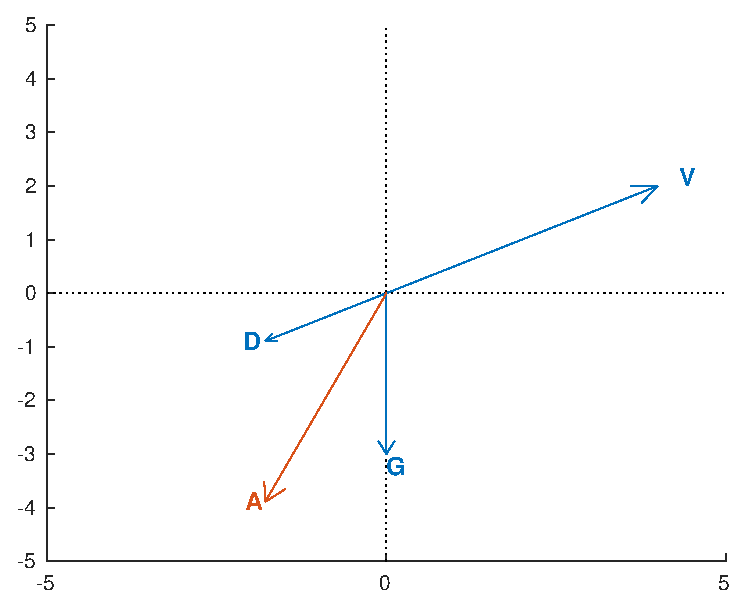
\includegraphics[height=3in]{figs/vector3.eps}}
\caption{Diagram of velocity, $\vec{V}$, acceleration due to drag force, 
$\vec{D}$, acceleration due to gravity, $\vec{G}$, and total acceleration, $\vec{A}$.}
\label{fig:vector3}
\end{figure}

Figure~\ref{fig:vector3} shows these quantities graphically.  Acceleration due to drag, $\vec{D}$, is in the opposite direction of velocity, $\vec{V}$.  Acceleration of gravity, $\vec{G}$, is straight down.  Total acceleration, $\vec{A}$, is the sum of $\vec{D}$ and $\vec{G}$.


\begin{figure}
\centerline{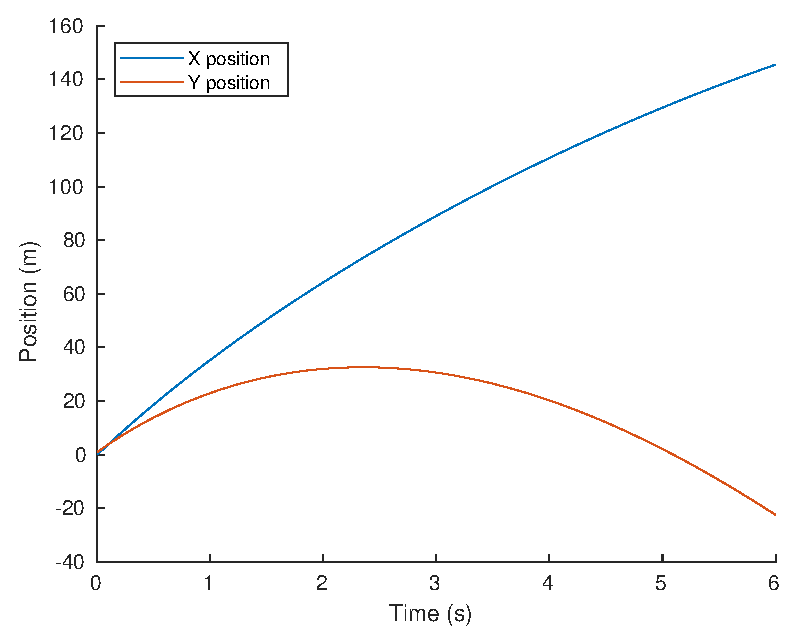
\includegraphics[height=3in]{figs/baseball2.eps}}
\caption{Simulated flight of a baseball including drag force.}
\label{fig:baseball2}
\end{figure}

Figure~\ref{fig:baseball2} shows the results from {\tt ode45}.  The ball lands after about \SI{5}{\second}, having traveled less than \SI{150}{\meter}, substantially less than what we got without air resistance, about \SI{250}{\meter}.

This result suggests that ignoring air resistance is not a good choice for modeling a baseball.


\section{What could go wrong?}

What could go wrong?  Well, {\tt vertcat} for one.  To explain
what that means, I'll start with {\bf concatenation}, which is
the operation of joining two matrices into a larger matrix.
``Vertical concatenation'' joins the matrices by stacking them on
top of each other; ``horizontal concatenation'' lays them
side by side.

Here's an example of horizontal concatenation with row vectors:

\begin{code}
>> x = 1:3
x = 1     2     3

>> y = 4:5
y = 4     5

>> z = [x, y]
z = 1     2     3     4     5
\end{code}

Inside brackets, the comma operator performs horizontal concatenation.
The vertical concatenation operator is the semi-colon.  Here is an
example with matrices:

\begin{code}
>> X = zeros(2,3)

X =  0     0     0
     0     0     0

>> Y = ones(2,3)

Y =  1     1     1
     1     1     1

>> Z = [X; Y]

Z =  0     0     0
     0     0     0
     1     1     1
     1     1     1
\end{code}

These operations only work if the matrices are the same size along
the dimension where they are glued together.  If not, you get:

\begin{code}
>> a = 1:3

a = 1     2     3

>> b = a'

b =  1
     2
     3

>> c = [a, b]
Error using horzcat
Dimensions of matrices being concatenated are not consistent.

>> c = [a; b]
Error using vertcat
Dimensions of matrices being concatenated are not consistent.
\end{code}

In this example, {\tt a} is a row vector and {\tt b} is a column
vector, so they can't be concatenated in either direction.

Reading the error messages, you probably guessed that {\tt horzcat}
is the function that performs horizontal concatenation, and likewise
with {\tt vertcat} and vertical concatenation.

In Section~\ref{sect:projectile} we use horizontal concatenation to packs {\tt dRdt} and {\tt dVdt} into the output variable:

\begin{code}
function res = rate_func(t, W)
    P = W(1:2);
    V = W(3:4);

    dPdt = V;
    dVdt = acceleration(t, P, V);

    res = [dPdt; dVdt];
end
\end{code}

As long as {\tt dRdt} and {\tt dVdt} are column vectors,
the semi-colon performs vertical concatenation, and the result is
a column vector with four elements.  But if either of them is a
row vector, that's trouble.

{\tt ode45} expects the result from \verb"rate_func" to be a
column vector, so if you are working with {\tt ode45}, it is
probably a good idea to make {\em everything} a column vector.

In general, if you run into problems with {\tt horzcat} and
{\tt vertcat}, use {\tt size} to display the dimensions of the operands,
and make sure you are clear on which way your vectors go.


\section{Glossary}

\begin{description}

\item[spatial vector:] A value that represents a
multidimensional physical quantity like position, velocity,
acceleration or force.

\item[unit vector:] A vector with norm 1, used to indicate
direction.

\item[norm:] The magnitude of a vector.  Sometimes called ``length,''
but not to be confused with the number of elements in a MATLAB
vector.

\item[concatenation:] The operation of joining two matrices end-to-end to
form a new matrix.

\end{description}


\section{Exercises}

\begin{ex}
When the Red Sox won the World Series in 2007, they played the
Colorado Rockies at their home field in Denver, Colorado.  Find an
estimate of the density of air in the Mile High City.  What effect
does this have on drag?  What effect does it have on the distance the baseball travels?
\end{ex}

\begin{ex}
The actual drag on a baseball is more complicated than what is
captured by our simple model.  In particular, the drag coefficient
depends on velocity.  You can get some of the details from {\em The
Physics of Baseball}\footnote{Robert K. Adair, Harper Paperbacks, 3rd
Edition, 2002.}; the figure you need is reproduced at \url{https://github.com/AllenDowney/ModSimMatlab/blob/master/code/data/baseball_drag.png}.

Use this data to specify a more realistic model of drag and modify your
program to implement it.  How big is the effect on the distance the baseball travels?
\end{ex}


\begin{ex}
\label{ex:cannon}
According to Wikipedia, the record distance for a human cannonball is 59.05 meters\footnote{See \url{https://en.wikipedia.org/wiki/Human_cannonball}.}.

Modify the example from this chapter to simulate the flight of a human cannonball.  You might have to do some research to find the drag coefficient and cross sectional area for a flying human.

Find the initial velocity (both magnitude and direction) you would need to break this record.  You might have to experiment to find the optimal launch angle.
\end{ex}





% ABD: I am commenting this out for now because the drag equation is
% probably not a good model for this scenario.

%\begin{ex}
%Suppose the baseball lands in a lake, and breaks the water's surface
%with velocity
%
%\begin{equation}
%    v_0 = (25, -25) ~  m/s
%\end{equation}
%
%How long will it take to resurface?
%
%Consider the baseball to be fully submerged when it enters the water. You will need to account for the gravitational force and the drag force (given in equation \eqref{eq:wikidrag}). You will also need to consider the force due to ``buoyancy'' which is given by Archimedes' principle:
%
%\begin{equation}
%    \vec{F_b} = \rho V g ~ \uvec{j}
%\end{equation}
%
%where $\rho$ is the density of the fluid (for water this is $1000 ~ kg /
%m^3$), $V$ is the volume of the fluid displaced (equal to the volume
%of the baseball---take this to be $0.000213 ~ m^3$), and $g$ the
%familiar gravitational constant; $\uvec{j}$ is the unit vector that
%points straight up:
%
%\begin{equation}
%    \uvec{j} = (0, 1)
%\end{equation}
%
%\end{ex}


% chap12
\chapter{Optimization}

In Exercise~\ref{ex:cannon}, you were asked to find the best launch angle for a human cannonball, meaning the angle that maximizes the distance traveled before landing.  In this chapter, we solve a similar problem, finding the best launch angle for a baseball.

We'll solve the problem two ways, first by running simulations with a range of values and plotting the results; then using a MATLAB function, {\tt fminsearch}.


\section{Optimal baseball}

In the previous chapter we wrote functions to simulate the flight of a baseball with a known initial velocity.  Now we'll use that code to find the launch angle that maximizes ``range'', that is, the distance the ball travels before landing.

First we need an event function to stop the simulation when the ball lands.

\begin{code}
function [value, isterminal, direction] = event_func(t, W)
    value = W(2);
    isterminal = 1;
    direction = -1;
end
\end{code}

This is similar to the event function we saw in Section~\ref{sect:events}, except that it uses {\tt W(2)} as the event value, which is the $y$ coordinate.  This event function stops the simulation when the altitude of the ball is 0 and falling.

Now we can call {\tt ode45} like this:

\begin{code}
    P = [0; 1];       % initial position in m
    V = [40; 30];     % initial velocity in m/s
    W = [P; V];       % initial condition
    
    tspan = [0 10];
    options = odeset('Events', @event_func);
    [T, M] = ode45(@rate_func, tspan, W, options);
\end{code}

The initial position of the ball is \SI{1}{\meter} above home plate.  Its initial velocity is \SI{40}{\meter\per\second} in the $x$ direction and \SI{30}{\meter\per\second} in the $y$ direction.

The maximum duration of the simulation is \SI{10}{\second}, but we expect an event to stop the simulation first.  We can get the final values of the simulation like this:
    
\begin{code}
    T(end)
    M(end, :)
\end{code}

The final time is \SI{5.1}{\second}.  The final $x$ position is \SI{131}{\meter}; the final $y$ position is 0, as expected.


\section{Trajectory}

Now we can extract the $x$ and $y$ positions:

\begin{code}
    X = M(:, 1);
    Y = M(:, 2);
\end{code}

In Section~\ref{sect:projectile} we plotted {\tt X} and {\tt Y} separately as functions of time.  Alternatively we can plot them against each other, like this:

\begin{code}
    plot(X, Y)
\end{code}

\begin{figure}
\centerline{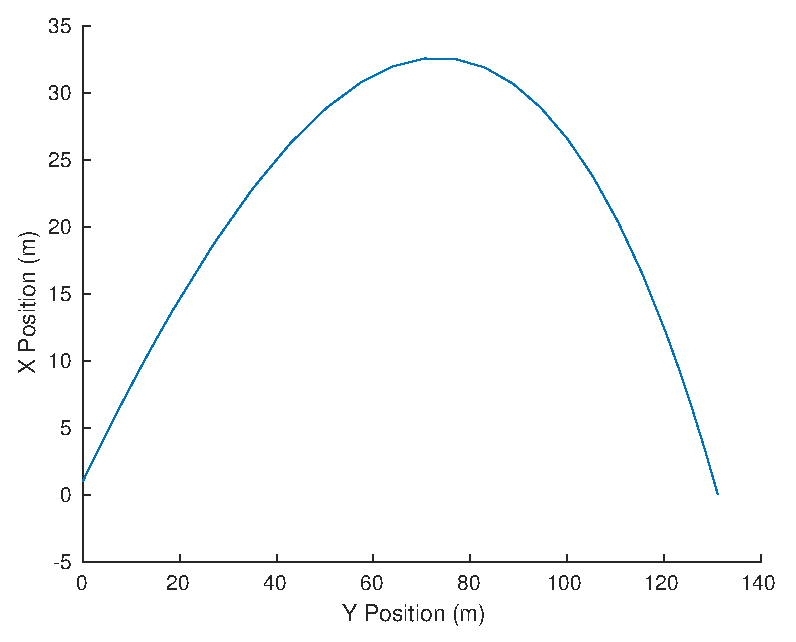
\includegraphics[height=3in]{figs/baseball3.eps}}
\caption{Simulated flight of a baseball plotted as a trajectory.}
\label{fig:baseball3}
\end{figure}

Figure~\ref{fig:baseball3} shows the result, which is the {\bf trajectory} of the baseball from launch, on the left, to landing, on the right.


\section{Range versus angle}

Now we'd like to simulate the trajectory of the baseball with a range of launch angles.  First, I'll take the code we have and wrap it in a function that takes the launch angle as an input variable, runs the simulation, and returns the distance the ball travels.

\begin{code}
function res = baseball_range(theta)
    P = [0; 1];       
    v = 50;           
    [vx, vy] = pol2cart(theta, v);
    
    V = [vx; vy];     % initial velocity in m/s
    W = [P; V];       % initial condition
    
    tspan = [0 10];
    options = odeset('Events', @event_func);
    [T, M] = ode45(@rate_func, tspan, W, options);
    
    res = M(end, 1);
end
\end{code}

The launch angle, {\tt theta}, is in radians.  The magnitude of velocity is always \SI{50}{\meter\per\second}.  I use {\tt pol2cart} to convert the angle and magnitude to Cartesian components, {\tt vx} and {\tt vy}.

After running the simulation, I extract the final $x$ position and return it as an output variable.  

We can run this function for a range of angles like this:

\begin{code}
    thetas = linspace(0, pi/2);
    for i = 1:length(thetas)
        ranges(i) = baseball_range(thetas(i));
    end
\end{code}

And then plot {\tt ranges} as a function of {\tt thetas}:

\begin{code}
    plot(thetas, ranges)
\end{code}

\begin{figure}
\centerline{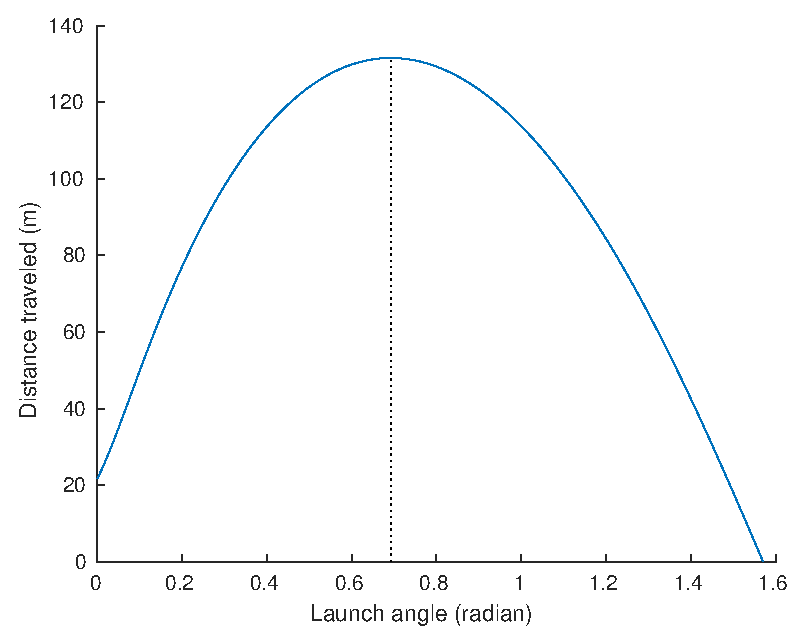
\includegraphics[height=3in]{figs/baseball4.eps}}
\caption{Simulated flight of a baseball plotted as a trajectory.}
\label{fig:baseball4}
\end{figure}

Figure~\ref{fig:baseball4} shows the result.  As expected, the ball does not travel far if it is hit nearly horizontal or vertical. 
The peak is apparently near \SI{0.7}{\radian}.

Considering that our model is only approximate, this result might be good enough.  But if we want to find the peak more precisely, we can use {\tt fminsearch}.


\section{{\tt fminsearch}}

{\tt fminsearch} is similar to {\tt fzero}, which we saw in Section\ref{sect:fzero}.  Recall that {\tt fzero} takes a function handle and an initial guess, and returns a root of the function.
As an example, to find a root of this function:

\begin{code}
function res = error_func(x)
    res = x^2 - 2;
end
\end{code}

We can call {\tt fzero} like this:

\begin{code}
>> x = fzero(@error_func, 1)
ans = 1.4142
\end{code}

The result is near the square root of 2.  If we call {\tt fminsearch} with the same function:

\begin{code}
>> x = fminsearch(@error_func, 1)
x = -8.8818e-16
\end{code}

The result is close to 0, which is where this function is minimized.  Optionally, {\tt fminsearch} returns two values:

\begin{code}
>> [x, fval] = fminsearch(@error_func, 1)
x = -8.8818e-16

fval = -2
\end{code}

{\tt x} is the location of the minimum; {\tt fval} is the value of the function evaluated at {\tt x}.

We can use {\tt fminsearch} to find the {\em maximum} of a function by writing a short function that negates the function we want to maximize:

\begin{code}
function res = min_func(angle)
    res = -baseball_range(angle);
end
\end{code}

Now we can call {\tt fminsearch} like this:

\begin{code}
>> [x, fval] = fminsearch(@min_func, pi/4)

x = 0.6921

fval = -131.5851
\end{code}

The optimal launch angle for the baseball is \SI{0.69}{\radian}; launched at that angle, the ball travels about \SI{132}{\meter}.

If you are curious about how {\tt fminsearch} works, see Section~\ref{sect:howfminsearch}.


\section{Animation}

Animation is a useful tool for checking the results of a physical
model.  If something is wrong, animation can make it obvious.
There are two ways to do animation in MATLAB.  One is to use
{\tt getframe} to capture a series of images and {\tt movie} to
play them back.

The more informal way is to draw a series of plots.  Here is a function that animates the results of a baseball simulation:

\begin{code}
function animate(T,M)
    X = M(:,1);
    Y = M(:,2);

    minmax = [min([X]), max([X]), min([Y]), max([Y])];

    for i=1:length(T)
        clf
        axis(minmax)
        plot(X(i), Y(i), 'o')
        drawnow;
        
        if i < length(T)
            dt = T(i+1) - T(i);
            pause(dt);
        end
    end
end
\end{code}

The input variables are the output from {\tt ode45}, a vector
{\tt T} and a matrix {\tt M}.  The columns of {\tt M} are the
$x$ and $y$ coordinates of the baseball.

{\tt minmax} is a vector of four elements which is used inside
the loop to set the axes of the figure.  This is necessary because
otherwise MATLAB scales the figure each time through the loop,
so the axes keep changing, which makes the animation hard
to watch.

Each time through the loop, {\tt animate} uses {\tt clf}
to clear the figure and {\tt axis} to reset the axes.  Then it plot a circle to represent the position of the baseball.

Each time through the loop, we have to call {\tt drawnow} so
that MATLAB actually displays each plot.  Otherwise it waits
until you finish drawing all the figures and {\em then} updates
the display.

We can call {\tt animate} like this:

\begin{code}
    tspan = [0 10];
    W = [0 1 30 40];
    [T, M] = ode45(@rate_func, tspan, W);
    animate(T, M)
\end{code}

One limitation of this kind of animation is that the speed
of the animation depends on how fast your computer can generate
the plots.  Since the results from {\tt ode45} are usually not
equally spaced in time, your animation might slow down where
{\tt ode45} takes small time steps and speed up where the time
step is larger.

One way to fix this problem is to change the way to specify {\tt tspan}.
Here is an example:

\begin{code}
    tspan = 0:0.1:10;
\end{code}

The result vector that goes from 0 to 10 with a
step size of 0.1.  This option does not affect the accuracy of the results; {\tt ode45} still uses variable time steps to generate the estimates, but then it interpolates them before returning the results.

With equal time steps, the animation should be smoother.

Another option is to use {\tt pause} to play the animation in
real time.  After drawing each frame and calling
{\tt drawnow}, you can compute the time
until the next frame and use {\tt pause} to wait:

\begin{code}
    dt = T(i+1) - T(i);
    pause(dt);
\end{code}

A limitation of this method is that it ignores the time required to
draw the figure, so it tends to run slow, especially if the figure is
complex or the time step is small.





\section{Exercises}



\begin{ex}
Manny Ramirez is a former member of the Boston Red Sox (an American baseball team) who was famous for his relaxed attitude.  The goal of this exercise is to solve the following Manny-inspired problem:

{\it What is the minimum effort required to hit a home run in Fenway Park?}

Fenway Park is a baseball stadium in Boston, Massachusetts.  One of its most famous features is the ``Green Monster", which is a wall in left field that is unusually close to home plate, only 310 feet away.  To compensate for the short distance, the wall is unusually high, at 37 feet.

\index{Ramirez, Manny}
\index{Fenway Park}
\index{baseball}
\index{Green Monster}
\index{velocity}

You can solve this problem in two steps:

\begin{enumerate}

\item For a given velocity, find the launch angle that maximizes the height of the ball when it reaches the wall.  Notice that this is not quite the same as the angle that maximizes the distance the ball travels.

\index{launch angle}

\item Find the minimal velocity that clears the wall, given that it has the optimal launch angle.  Hint: this is actually a root-finding problem, not an optimization problem.

\end{enumerate}

\end{ex}

\begin{ex}
\label{ex:golf}

A golf ball hit with backspin generates lift, which might increase the distance it travels, but the energy that goes into generating spin probably comes at the cost of lower initial velocity.

Write a simulation of the flight of a golf ball and use it to find
the launch angle and allocation of spin and initial velocity
(for a fixed energy budget) that maximizes the horizontal range of the
ball in the air.

The lift of a spinning ball is due to the Magnus force\footnote{See
\url{https://en.wikipedia.org/wiki/Magnus_effect}.}, which is
perpendicular to the axis of spin and the path of flight.  The
coefficient of lift is proportional to the spin rate; for a ball
spinning at 3000 rpm it is about 0.1.  The coefficient of drag of a
golf ball is about 0.2 as long as the ball is moving faster than \SI{20}{\meter\per\second}.

\end{ex}


\chapter{Case studies}

This chapter includes additional exercises where you can apply what you have learned.

\section{Celestial mechanics}

{\bf Celestial mechanics} describes how objects move in outer space.
If you did Exercise~\ref{ex:earth}, you simulated the Earth being pulled toward the Sun in one dimension.  Now we'll simulate the Earth orbiting the Sun in two dimensions.

To keep things simple, we'll consider only the effect of the Sun on the Earth, and ignore the effect of the Earth on the Sun.  So we'll place the Sun at the origin and use a spatial vector, $\vec{P}$, to represent the position of the Earth relative to the Sun.

Given the mass of the Sun, $m1$, and the mass of the Earth, $m2$, the gravitational force between them is

\begin{equation*}
\vec{F_g} = -G \frac{m_1 m_2}{r^2} \uvec{P}
\end{equation*}

where $G$ is the universal gravitational constant\footnote{See \url{https://en.wikipedia.org/wiki/Gravity}.},
$r$ is the distance of Earth from the Sun, and
$\uvec{P}$ is a unit vector in the direction of $\vec{P}$.

Write a simulation of Earth orbiting the Sun.  You can look up the orbital velocity of the Earth, or search for the initial velocity that causes the earth to make one complete orbit in one year.  Optionally, use {\tt fminsearch} to find the velocity that gets the Earth as close as possible to the starting place after one year.



\section{Conservation of Energy}

A useful way to check the accuracy of an ODE solver is to see whether it conserves energy.  For planetary motion, it turns out that {\tt ode45} does not.

The kinetic energy of a moving body is

\begin{equation*}
KE = m v^2 / 2
\end{equation*}

The potential energy of a sun with mass $m_1$ and a
planet with mass $m_2$ and a distance $r$ between them is

\begin{equation}
PE = -G \frac{m_1 m_2}{r}
\end{equation}

Write a function called {\tt energy\_func} that takes the output of
your Earth simulation and computes the total
energy (kinetic and potential) of the system for each estimated
position and velocity.

Plot the result as a function of time and
check whether it increases or  decreases over the course of the simulation.

You can reduce the rate of energy loss by decreasing {\tt ode45}'s
tolerance option using {\tt odeset} (see Section~\ref{sect:events}):

\begin{code}
options = odeset('RelTol', 1e-5);
[T, M] = ode45(@rate_func, tspan, W, options);
\end{code}

The name of the option is {\tt RelTol} for ``relative tolerance.''
The default value is {\tt 1e-3} or 0.001.  Smaller values
make {\tt ode45} less ``tolerant,'' so it does more work to
make the errors smaller.

Run {\tt ode45} with a range of values for {\tt RelTol} and confirm
that as the tolerance gets smaller, the rate of energy loss
decreases.

Along with {\tt ode45}, MATLAB provides several other ODE solvers (see \url{https://www.mathworks.com/help/matlab/math/choose-an-ode-solver.html}).
Run your simulation with one of the other ODE solvers MATLAB provides
and see if any of them conserve energy.  You might find that {\tt ode23} works surprisingly well (although technically it does not conserve energy either).


\section{Bungee jumping}
\label{bungee}

Suppose you want to set the world record for the highest ``bungee dunk", which is a stunt in which a bungee jumper dunks a cookie in a cup of tea at the lowest point of a jump.  An example is shown in this video: \url{http://modsimpy.com/dunk}.

Since the record is \SI{70}{\meter}, let's design a jump for \SI{80}{\meter}.  We'll start with the following modeling assumptions:

\begin{itemize}

\item  Initially the bungee cord hangs from a crane with the attachment point \SI{80}{\meter} above a cup of tea.

\item Until the cord is fully extended, it applies no force to the jumper.  It turns out this might not be a good assumption; we will revisit it.

\item After the cord is fully extended, it obeys Hooke's Law; that is, it applies a force to the jumper proportional to the extension of the cord beyond its resting length.  See \url{http://modsimpy.com/hooke}. 

\item The mass of the jumper is \SI{75}{\kilogram}.

\item The jumper is subject to drag force, as in the previous model, so that their terminal velocity is \SI{60}{\meter \per \second}.

\end{itemize}

Our objective is to choose the length of the cord, {\tt L}, and its spring constant, {\tt k}, so that the jumper falls all the way to the tea cup, but no farther!

We'll start with the length of the bungee cord, {\tt L} at \SI{25}{\meter} and spring constant, {\tt k} at \SI{40}{\newton \per \meter}.

Assume that the jumper has a cross-sectional area of \SI{1}{\meter} and a terminal velocity of \SI{60}{\meter\per\second}, and weighs \SI{75}{\kilogram}.


\section{Bungee revisited}

In the previous case study we simulated a bungee jump with a model that took into account gravity, air resistance, and the spring force of the bungee cord, but we ignored the weight of the cord.

\index{bungee jump}
\index{bungee cord}

It is tempting to say that the cord has no effect because it falls along with the jumper, but that intuition is incorrect.  As the cord falls, it transfers energy to the jumper.

At \url{http://modsimpy.com/bungee} you'll find a paper\footnote{Heck, Uylings, and Kedzierska, ``Understanding the physics of bungee jumping", Physics Education, Volume 45, Number 1, 2010.} that explains this phenomenon and derives the acceleration of the jumper, $a$, as a function of position, $y$, and velocity, $v$:
%
\[ a = g + \frac{\mu v^2/2}{\mu(L+y) + 2L} \] 
%
where $g$ is acceleration due to gravity, $L$ is the length of the cord, and $\mu$ is the ratio of the mass of the cord, $m$, and the mass of the jumper, $M$.

If you don't believe that their model is correct, this video might convince you: \url{http://modsimpy.com/drop}.

Modify your solution to the previous problem to model this effect.  How does the behavior of the system change as we vary the mass of the cord?  When the mass of the cord equals the mass of the jumper, what is the net effect on the lowest point in the jump?


\section{Spider-Man}

In this case study we'll develop a model of Spider-Man swinging from a
springy cable of webbing attached to the top of the Empire State
Building.  Initially, Spider-Man is at the top of a nearby building, as
shown in Figure~\ref{spiderman}.

\index{Spider-man}
\index{Empire State Building}

\begin{figure}
\centerline{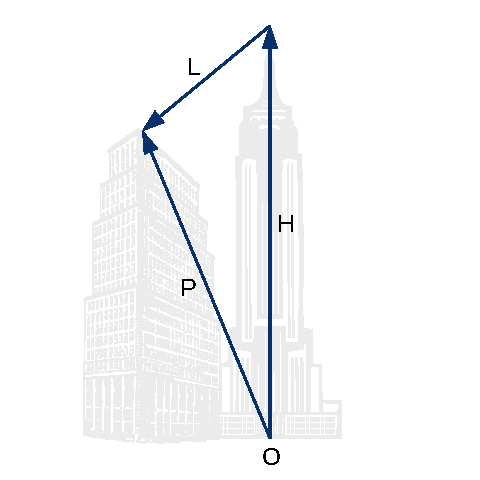
\includegraphics[height=2.5in]{figs/spiderman.pdf}}
\caption{Diagram of the initial state for the Spider-Man case study.}
\label{spiderman}
\end{figure}

The origin, {\tt O}, is at the base of the Empire State Building. The
vector {\tt H} represents the position where the webbing is attached
to the building, relative to {\tt O}. The vector {\tt P} is the
position of Spider-Man relative to {\tt O}. And {\tt L} is the
vector from the attachment point to Spider-Man.

\index{vector}

By following the arrows from {\tt O}, along {\tt H}, and along
{\tt L}, we can see that

\begin{code}
H + L = P
\end{code}

So we can compute {\tt L} like this:

\begin{code}
L = P - H
\end{code}

The goals of this case study are:

\begin{enumerate}

\item
  Implement a model of this scenario to predict Spider-Man's trajectory.
\index{trajectory}

\item
  Choose the right time for Spider-Man to let go of the webbing in order
  to maximize the distance he travels before landing.
\index{range}

\item
  Choose the best angle for Spider-Man to jump off the building, and let
  go of the webbing, to maximize range.
\index{optimization}  
  
\end{enumerate}

We'll use the following parameters:
\index{parameter}

\begin{enumerate}

\item According to the Spider-Man Wiki\footnote{\url{http://modsimpy.com/spider}}, Spider-Man weighs \SI{76}{\kg}.

\item
  Let's assume his terminal velocity is \SI{60}{\meter\per\second}.
\index{terminal velocity}

\item
  The length of the web is \SI{100}{\meter}.

\item
  The initial angle of the web is \SI{45}{\degree} to the left of straight
  down.

\item
  The spring constant of the web is \SI{40}{\newton\per\meter} when the cord is stretched, and 0 when it's compressed.

\end{enumerate}



%chap14
\chapter{How does it work?}

In this chapter we ``open the hood'', looking more closely at how some of the tool we have used --- {\tt ode45}, {\tt fzero}, and {\tt fminsearch} --- work.


\section{How {\tt ode45} works}
\label{sect:howode45}

According to the MATLAB documentation, {\tt ode45} uses ``an explicit Runge-Kutta formula, the Dormand-Prince pair''.  You can read about it at \url{https://en.wikipedia.org/wiki/Runge-Kutta_methods}, but I'll try to give you a sense of it here.

The key idea behind all Runge-Kutta methods is to evaluate the rate function several times at each time step, and use a weighted average of the computed slopes to estimate the value at the next time step.  The details are in where the rate function is called and how the slopes are averages.

As an example, I'll solve the following differential equation:

\[ \frac{dy}{dt}(t) = y \sin t \] 

Given a differential equation, it is usually straightforward to write a rate function:

\begin{code}
function res = rate_func(t, y)
    dydt = y * sin(t);
    res = dydt;
end
\end{code}

And we can call it like this:

\begin{code}
    y0 = 1;
    tspan=[0 4];
    options = odeset('Refine', 1);
    [T, Y] = ode45(@rate_func, tspan, y0, options);
\end{code}

For this example I use {\tt odeset} to set the {\tt Refine} option to 1, which tells {\tt ode45} to return only the time steps it computed, rather than interpolating between them.

Now I can modify the rate function to plot the places where it gets evaluated:

\begin{code}
function res = rate_func(t, y)
    dydt = y * sin(t);
    res = dydt;

    plot(t, y, 'ro')
    dt = 0.01;
    ts = [t t+dt];
    ys = [y y+dydt*dt];
    plot(ts, ys, 'r-')
end
\end{code}

Now when \verb"rate_func" runs it plot a red circle at each location, and a short red line showing the computed slope.

Figure~\ref{fig:odeplot1} shows the result.  {\tt ode45} computes 10 time steps (not counting the initial condition) and evaluates the rate function 61 times.

\begin{figure}
\centerline{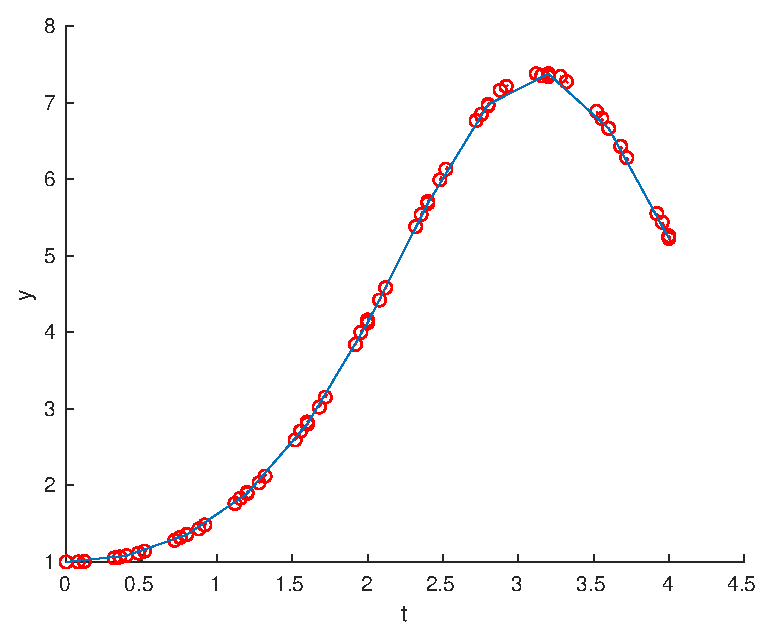
\includegraphics[height=3in]{figs/odeplot1.eps}}
\caption{Points where {\tt ode45} evaluates the rate function.}
\label{fig:odeplot1}
\end{figure}

Figure~\ref{fig:odeplot2} shows the same plot, zoomed in on a single time step, from $0.8$ to $1.2$.  We can see that {\tt ode45} evaluates the rate function several times per time step, at several times between the end points.  

\begin{figure}
\centerline{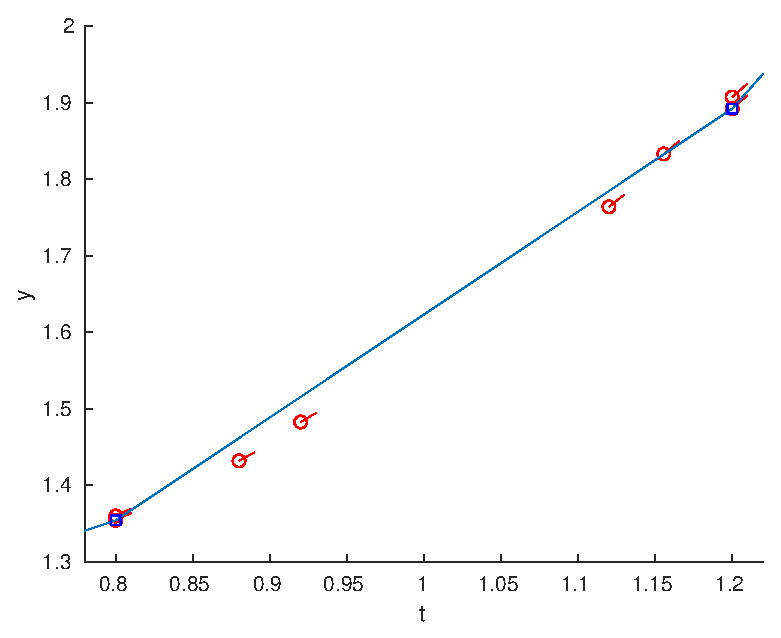
\includegraphics[height=3in]{figs/odeplot2.eps}}
\caption{Points where {\tt ode45} evaluates the rate function, zoomed in.}
\label{fig:odeplot2}
\end{figure}

One important thing to take away from this figure: most of the places where {\tt ode45} evaluates the rate function are not part of the solution it returns, and they are not always good estimates of the solution.



\section{How {\tt fzero} works}
\label{sect:howfzero}

According to the MATLAB documentation, {\tt fzero} uses uses ``a combination of bisection, secant, and inverse quadratic interpolation methods''.

To understand what that means, suppose we are trying to find a root of a function on one variable, $f(x)$, and assume we have evaluated the function at two place, $x_1$ and $x_2$, and found that the result have opposite signs.  Specifically, assume $f(x_1) > 0$ and $f(x_2) < 0$, as shown in Figure~\ref{fig:secant}.

\begin{figure}
\centerline{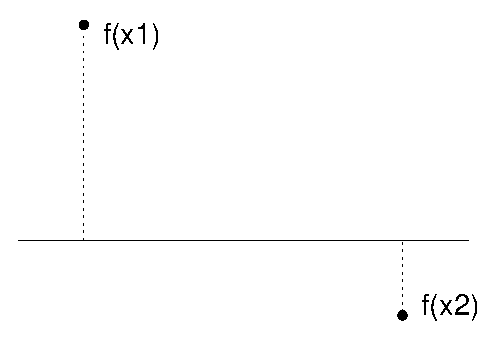
\includegraphics[height=1.1in]{figs/secant.eps}}
\caption{Initial state of a root-finding search.}
\label{fig:secant}
\end{figure}

As long as $f$ is continuous, there must be at least one root in this interval.  In this case we would say that $x_1$ and $x_2$
{\bf bracket} a zero.

If this was all you knew about $f$, where would you go looking for
a root?  If you said ``halfway between $x_1$ and $x_2$'',
congratulations!  You just invented a numerical method called
{\bf bisection}!

If you said, ``I would connect the dots with a straight line
and compute the zero of the line,''
congratulations!  You just invented the {\bf secant method}!

And if you said, ``I would evaluate $f$ at a third point, find the
parabola that passes through all three points, and compute the zeros
of the parabola,'' then congratulations, you just invented inverse quadratic interpolation.

That's most of how {\tt fzero} works.  The details of how these methods are combined are interesting, but beyond the scope of this book.  You can read more at \url{https://en.wikipedia.org/wiki/Brents_method}.  


\section{How {\tt fminsearch} works}
\label{sect:howfminsearch}

According to the MATLAB documentation, {\tt fminsearch} uses the Nelder-Mead simplex algorithm.  You can read about it at \url{https://en.wikipedia.org/wiki/Nelder-Mead_method}, but you might find it overwhelming.

To give you a sense of how it works, I will present a simpler algorithm, the {\bf golden-section search}.  Suppose we are trying to find the minimum of a function of a single variable, $f(x)$.  As a starting place, assume that we have evaluated the function at three places, 
$x_1$, $x_2$, and $x_3$, and found that $x_2$ yields the lowest
value. Figure~\ref{fig:golden1} shows this initial state.

\begin{figure}
\centerline{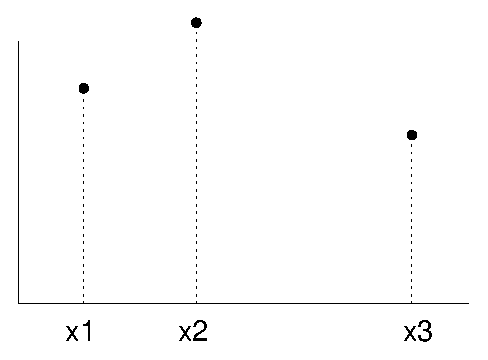
\includegraphics[height=1.1in]{figs/golden1.eps}}
\caption{Initial state of a golden-section search.}
\label{fig:golden1}
\end{figure}

If $f$ is continuous, there has to be at least one
minimum point between $x_1$ and $x_3$.

The next step is to choose a fourth point, $x_4$, and evaluate
$f(x_4)$.  There are two possible outcomes, depending on whether
$f(x_4)$ is greater than $f(x_2)$.
Figure~\ref{fig:golden2} shows the two possible states.

\begin{figure}
\centerline{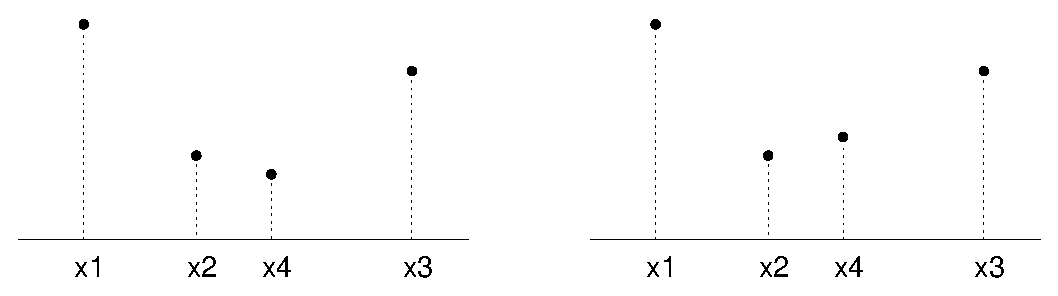
\includegraphics[height=1.1in]{figs/golden2.eps}}
\caption{Possible states of a golden-section search after evaluating $f(x_4)$.}
\label{fig:golden2}
\end{figure}

If $f(x_4)$ is less than than $f(x_2)$ (shown on the left), the
local minimum must be between $x_2$ and $x_3$, so we would discard $x_1$ and proceed with the new triple $(x_2, x_4, x_3)$.

If $f(x_4)$ is greater than $f(x_2)$ (shown on the right), the
local minimum must be between $x_1$ and $x_4$, so we would discard $x_3$ and proceed with the new triple $(x_1, x_2, x_4)$.

Either way the range gets smaller and our estimate of the optimal value of $x$ gets better.

This method works for almost any value of $x_4$, but some choices
are better than others.  You might be tempted to bisect the interval between $x_2$ and $x_3$, but that turns out not to be the best choice.  You can read about a better option at \url{https://en.wikipedia.org/wiki/Golden-section_search#Probe_point_selection}.



\begin{appendices}
\chapter{The Theorems of Debugging}

\begin{enumerate}
    \item \displaythrm{1}
    \item \displaythrm{2}
    \item \displaythrm{3}
    \item \displaythrm{4}
    \item \displaythrm{5}
    \item \displaythrm{6}
    \item \displaythrm{7}
    \item \displaythrm{8}
    %\item \displaythrm{9}
\end{enumerate}

\end{appendices}

% Print the index
\printindex


\end{document}




But sometimes 
if the error messages make
suggestions about what to change,
it can be risky to follow those suggestions.  If you do what you're told, you
might make the error messages go away, but that doesn't mean the
program will do the right thing.  MATLAB doesn't know what the program
is {\em supposed} to do, but you should.

And that brings us to the Eighth Theorem of Debugging:

\begin{quote}
\displaythrm{8}
\end{quote}


\section{Dot and cross products}

Multiplying a vector by a scalar is a straightforward operation;
so is adding two vectors.  But multiplying two vectors is more
subtle.  It turns out that there are two vector operations that
resemble multiplication: the {\bf dot product}
and the {\bf cross product}.

The dot product of vectors $\vec{u}$ and $\vec{v}$ is a scalar:\index{Spatial vectors!dot product}

\begin{equation}
    \vec{u} \cdot \vec{v} = \norm{\vec{u}} \norm{\vec{v}} \cos \theta
\end{equation}

where $\theta$ is the smallest angle between $\vec{u}$ and
$\vec{v}$. We already know how to compute magnitudes, and you could
probably figure out how to compute $\theta$, but you don't have to.
MATLAB provides a function, {\tt dot}, that computes dot products:

\begin{code}
d = dot(U, V)
\end{code}

{\tt dot} works in any number of dimensions, as long as {\tt U}
and {\tt V} have the same number of elements.

If one of the operands is a unit vector, you can use the dot
product to compute the component of a vector $\vec{u}$ that is in
the direction of a unit vector, $\uvec{r}$:

\begin{code}
s = dot(U, Rhat)
\end{code}

In this example, $s$ is the {\bf scalar projection} of $\vec{u}$
onto $\uvec{r}$.  The {\bf vector projection} is the vector
that has magnitude $s$ in the direction of $\uvec{r}$:

\begin{code}
V = dot(U, Rhat) * Rhat
\end{code}

The cross product of vectors $\vec{u}$ and $\vec{v}$ is a vector whose
direction is perpendicular to $\vec{u}$ and $\vec{v}$
(with orientation determined by the right-hand
rule\footnote{\url{https://en.wikipedia.org/wiki/Right-hand_rule}})
and whose magnitude is\index{Spatial vectors!cross product}

\begin{equation}
    \norm{\vec{u} \times \vec{v}} = \norm{\vec{u}} \norm{\vec{v}} \sin \theta
\end{equation}

where (again) $\theta$ is the smallest angle between $\vec{u}$ and
$\vec{v}$. MATLAB provides a function, {\tt cross}, that computes cross
products.

\begin{code}
C = cross(U, V)
\end{code}

{\tt cross} calculates the cross product of corresponding vectors along
the first array dimension whose size equals 3.

A common use of {\tt cross} is to compute torques.  If you represent
a moment arm $\vec{R}$ and a force $\vec{F}$ as vectors with size equal
to 3, then the torque is just

\begin{code}
Tau = cross(R, F)
\end{code}

If the components of {\tt R} are in meters and the components
of {\tt F} are in Newtons, then the torques in {\tt Tau} are
in Newton-meters.


% \section{Scaling}

% \section{Polar coordinates}

\section{What is a model for?}

In Section~\ref{sect:modeling} I defined a ``model'' as a simplified
description of a physical system, and said that a good model
lends itself to analysis and simulation, and makes predictions
that are good enough for the intended purpose.

Since then, we have seen a number of examples; now we can
say more about what models are for.  The goals of a model tend
to fall into three categories.

\begin{description}

\item[prediction:] Some models make predictions about physical
systems.  As a simple example, the duck model in
Exercise~\ref{ex:duck} predicts the level a duck floats at.  At the other
end of the spectrum, global climate models try to predict the weather
tens or hundreds of years in the future.

\item[design:] Models are useful for engineering design, especially
for testing the feasibility of a design and for optimization.  For
example, in Exercise~\ref{ex:golf} you were asked to design the golf
swing with the perfect combination of launch angle, velocity and spin.

\item[explanation:] Models can answer scientific questions.  For
example, the Lotka-Volterra model in Section~\ref{sect:lotka} offers a
possible explanation of the dynamics of animal populations systems in
terms of interactions between predator and prey species.

\end{description}

The exercises at the end of this chapter include one model of
each type.


\section{Glossary}

\begin{description}

\item[dot product:] A scalar product of two vectors, proportional to the
norms of the vectors and the cosine of the smallest angle between them.

\item[cross product:] A vector product of two vectors with norm
proportional to the norms of the vectors and the sine of the angle
between them, and direction perpendicular to both.

\item[projection:] The component of one vector that is in the
direction of the other (might be used to mean ``scalar projection'' or
``vector projection'').

\end{description}

\chapter{Nested Functions}
\label{chpt:nestedfuns}
\index{Functions!nested}

This appendix provides an alternative way to structure code that
involves helper functions, which were discussed in Section~\ref{sect:funfiles};
there, we saw an example of an M-file with more than one function:

\begin{code}
function res = duck()
    error = error_func(10)
end

function res = error_func(h)
    rho = 0.3;      % density in g / cm^3
    r = 10;         % radius in cm
    res = ...
end
\end{code}

Because the first function ends before the second begins, these
functions are at the same level of indentation.  Functions like
these are parallel, as opposed to nested.  A nested function is
defined inside another, like this:

\begin{code}
function res = duck()
    error = error_func(10)

    function res = error_func(h)
        rho = 0.3;      % density in g / cm^3
        r = 10;         % radius in cm
        res = ...
    end
end
\end{code}

The function {\tt duck} is the enclosing function and {\tt
error\_func} is the nested function.

Nesting functions is useful because the variables of the outer
function can be accessed from the inner function.  This is not
possible with parallel functions.

In this example, using a nested function makes it possible to
move the parameters {\tt rho} and {\tt r} out of {\tt error\_func}.

\begin{code}
function res = duck(rho)
    r = 10;
    error = error_func(10)

    function res = error_func(h)
        res = ...
    end
end
\end{code}

Both {\tt rho} and {\tt r} can be accessed from {\tt error\_func}.
By making {\tt rho} an input argument, we made it easier to test
{\tt duck} with different parameter values.

Nested functions can also help de-clutter code (but not always). For
more information on nested functions, please consult the official documentation
at \url{https://www.mathworks.com/help/matlab/matlab_prog/nested-functions.html}.
